\documentclass{beamer}
\input{../style/cours-style.sty}

% Title
\title[JavaScript]{JavaScript Frontend - B1 Web et Multimédia}
\author{Christophe Brun}
\institute{My Digital School}
\beamertemplatenavigationsymbolsempty

% JS scpécific listing inspired by https://tex.stackexchange.com/questions/89574/language-option-supported-in-listings
\definecolor{lightgray}{rgb}{.9,.9,.9}
\definecolor{darkgray}{rgb}{.4,.4,.4}
\definecolor{purple}{rgb}{0.65, 0.12, 0.82}
\definecolor{silver}{RGB}{236, 240, 241}

\lstdefinelanguage{JavaScript}{
    keywords={typeof, new, true, false, try, catch, function, return, null, async, await, switch, var, const, let, if, in, while, for, do, else, case, break, undefined, default, continue},
    keywordstyle=\color{blue}\bfseries,
    ndkeywords={class, export, boolean, throw, implements, import, this},
    ndkeywordstyle=\color{darkgray}\bfseries,
    identifierstyle=\color{black},
    sensitive=false,
    comment=[l]{//},
    morecomment=[s]{/*}{*/},
    commentstyle=\color{purple}\ttfamily,
    stringstyle=\color{red}\ttfamily,
    morestring=[b]',
    morestring=[b]"
}

\lstset{
    language=JavaScript,
    basicstyle=\ttfamily\scriptsize,
    backgroundcolor=\color{silver},
    keywordstyle=\color{flatgreen},        % Keywords font ('*' = uppercase)
    commentstyle=\color{flatblue},         % Step between two line-numbers
    columns=fullflexible,
    breaklines=true,
    showstringspaces=false % Mandatory to display spaces in strings with Roboto font
}

\lstdefinestyle{JavaScript}{
    language=JavaScript,
    style=JSES6Base
}
\lstdefinestyle{ES6}{
    language=ES6,
    style=JSES6Base
}
\titlegraphic{
    \bigbreak
    
\includegraphics[width=5cm]{image/mds-logo}
    \bigbreak
    L’école des métiers du digital
    \bigbreak
}

\begin{document}

    \begin{frame}
        \titlepage
        \bigbreak
        \centering
        \url{https://github.com/My-Digital-School-by-PapIT/frontend-JS}
    \end{frame}


    \section{Table des matières}\label{sec:toc}

    \begin{frame}{Table des matières}
        \begin{tiny}
            \begin{multicols}{1}
                \tableofcontents
            \end{multicols}
        \end{tiny}
    \end{frame}


    \section{Programme du module}\label{sec:programme-du-module}

    \begin{frame}{JavaScript Frontend}{Objectifs des 6 jours}
        \begin{columns}
            \column{0.7\textwidth}
            \begin{scriptsize}
                \begin{itemize}
                    \item Distinguer les différentes parties prenantes du web (protocol de communication,
                    navigateur, serveur, \textit{etc}).
                    \item La syntaxe JavaScript.
                    \item La Window API, manipulation de DOM.
                    \item Intéragir avec une API depuis le frontend.
                \end{itemize}
            \end{scriptsize}
            \column{0.3\textwidth}
            
\includegraphics[width=4cm]{image/js-surfing}
        \end{columns}
    \end{frame}


    \section{Introduction}\label{sec:introduction}

    \begin{frame}{Formateur sur JS}{Christophe Brun, conseil en développement informatique}

        \begin{columns}
            \column{0.7\textwidth}
            \begin{itemize}
                \item Développeur freelance (Python, Java, JS, CoBOL) et data at scale.

                \item 7 ans de conseil en développement au sein d'SSII~.

                \item 7 ans de conseil en développement en indépendant, \href{https://papit.fr}{PapIT}.

                \item Passionné~! \bigbreak
                \begin{columns}
                    \column{0.5\textwidth}
                    \centering
                    
\includegraphics[width=3cm]{image/logo-uppa}
                    \column{0.5\textwidth}
                    \centering
                    
\includegraphics[width=3cm]{image/logo-universite-bordeaux}
                \end{columns}
            \end{itemize}
            \column{0.3\textwidth}
            \centering
            
\includegraphics[width=5cm]{image/trombine-christophe}
        \end{columns}
    \end{frame}


    \section{Les ressources du Web}\label{sec:ressources}

    \begin{frame}{Les ressources du Web}{Dvisions en briques}
        \begin{columns}
            \column{0.6\textwidth}
            1 des 4 règles pour la direction de l'esprit de Descartes~: \textquote{Diviser chacune des difficultés que j'examinerais, en autant de parcelles qu'il se pourrait et qu'il serait requis pour les mieux résoudre.}.
            \column{0.4\textwidth}
            \centering
            
\includegraphics[width=6cm]{image/Descartes}
        \end{columns}
    \end{frame}

    \begin{frame}{Les ressources du Web}{Analyse des composants}
        \centering
        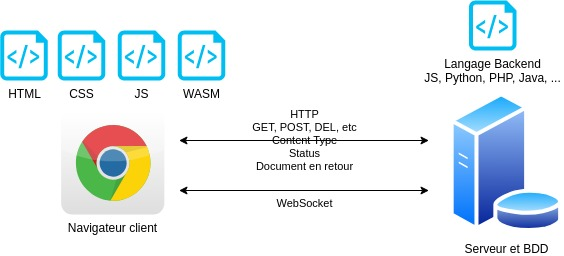
\includegraphics[width=11cm]{image/web-stakeholders.drawio}
    \end{frame}


    \section{Le web statique}\label{sec:static}

    \begin{frame}{Le web statique}
        Une des premières options pour un site web est donc d'être statique.

        Suite à une requête sur une URL (adresse dans le navigateur), le serveur nous
        envoie une page HTML pour la donnée avec du CSS pour le style. \bigbreak Il n'y
        a pas d'interaction avec le serveur, le contenu est figé, on peut juste passer
        à une autre page grâce à une ancre \lstinline{<a href="...">...</a>}. \bigbreak
        \centering 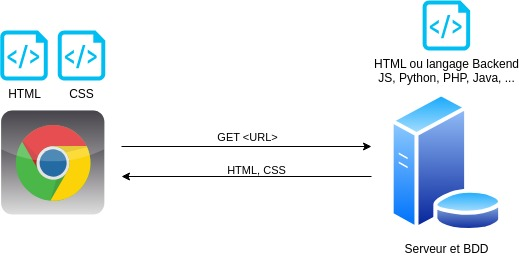
\includegraphics[width=8cm]{image/web-static}
    \end{frame}

    \begin{frame}[fragile]{Développement Web Statique}{Exercice \execcounterdispinc{}}
        \begin{itemize}
            \item Installer Python 3.
            \item Installer un IDE de développement Web comme WebStorm.
            \item Lancer un serveur HTTP avec la commande dans le répertoire du cours~:
            \begin{lstlisting}[language=Bash,title={\tiny{Commande dans un Shell/Console/PowerShell}}]
python3 -m http.server
            \end{lstlisting}
            \item Naviguer à l'adresse indiquée.
            \item Modifier le fichier \lstinline{index.html} pour ajouter un lien vers une page
            HTML développée par vos soins avec votre nom et une photo de vous.
            \item Rafraîchir la page et vérifier que la modification est fonctionnelle.
        \end{itemize}
    \end{frame}


    \section{Le web dynamique}\label{sec:Dynamic}
    \begin{frame}{Développement Web Dynamique}{Exercice \execcounterdispinc{}}
        \begin{itemize}
            \item Quelles seraient les moyens d'avoir des pages web dynamiques~?
        \end{itemize}
        \bigbreak
        \centering
        
\includegraphics[width=5cm]{image/question-mark}
    \end{frame}

    \begin{frame}{Développement Web Dynamique}{Backend}
        Un serveur qui fait tourner un algorithme qui sert des données qui évoluent (dans la base de données), ou de l'extérieur (API).

        Plusieurs requêtes sont nécessaires, de différents types~:
        \begin{itemize}
            \item Des GET comme auparavant pour retourner des données.
            \item Des POST pour envoyer des données au serveur.
            \item Des DEL pour supprimer des données de la base de données du serveur.
        \end{itemize}
        \bigbreak
        \centering
        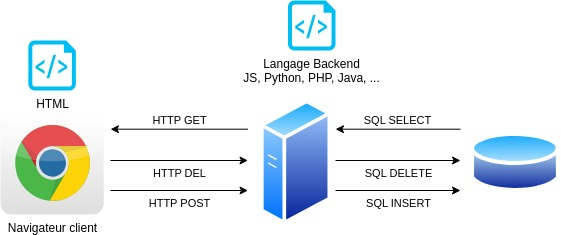
\includegraphics[width=7cm]{image/web-dynamic-backend}
    \end{frame}

    \begin{frame}{Frontend}
        \begin{small}
            Il est également possible de modifier une page web sans recharger la page entière, en utilisant JavaScript.

            Le JavaScript est un des langages qui peut être interprétés par le navigateur.

            Ces langages sont~:
            \begin{itemize}
                \item \textbf{HTML}, un langage de balisage, à l'image du XML, c'est le document principal de la page.
                Il peut contenir de la mise en forme, des données à afficher, \textit{etc}.
                \item \textbf{CSS}, un langage de style, qui permet de définir la mise en forme de la page.
                C'est une manière \textbf{modulaire} de définir le style de tout un site web.
                \item \textbf{JavaScript}, un langage de programmation qui permet de modifier le contenu de la page sans recharger la page.
                Il peut modifier~:
                \begin{itemize}
                    \item Le contenu de la page, ses données (DOM API\footnotemark{}).
                    \item Le style de la page, la mise en forme (DOM API\cref{DOM}).
                    \item Intéragir avec n'importe quel serveur.
                \end{itemize}
            \end{itemize}
        \end{small}
        \footnotetext{\label{DOM}DOM (Document Object Model), \url{https://developer.mozilla.org/fr/docs/Glossary/DOM}}
    \end{frame}


    \section{Généralité sur le JavaScript en Frontend}\label{sec:js-basic}

    \subsection{Où est-il~?}\label{sec:where}

    \begin{frame}{Où se trouve le JavaScript ?}
        Deux solutions, ils se trouvent~:
        \begin{itemize}
            \item Dans le fichier HTML, entre les balises \lstinline{<script>...</script>}.
            \item Dans un fichier séparé, avec l'attribut
            \lstinline{src} de la balise \lstinline{<script>} qui indique le chemin de ce
            fichier. Comme le fichier de style, cette méthode est plus modulaire, car ce
            fichier peut être partagé entre plusieurs pages.
            Ces balises \lstinline{<script>} doivent être placées à la fin du \lstinline{<body>}.
        \end{itemize}
        \bigbreak
        \begin{dangercolorbox}
            En programmation, être modulaire est une qualité importante. Si on réutilise, on est écrit moins.
            Ici, dans un seul fichier.
            Si on écrit moins, on écrit moins de bug~!
        \end{dangercolorbox}
    \end{frame}

    \begin{frame}{Exercice \execcounterdispinc{}}
        \begin{itemize}
            \item Trouver le Script JavaScript du fichier \lstinline{index.html}.
            \item Créer un fichier
            \lstinline{script.js} dans le même répertoire que \lstinline{index.html}.
            \item Copier le contenu du script dans ce fichier.
            \item Adapter le fichier
            \lstinline{index.html} pour inclure ce fichier en utilisant l'attribut \lstinline{src}
            et supprimant le contenu de la balise qui devient inutile.
            \item Simplifier la balise \lstinline{<script>} en conséquence.
            \item Rafraîchir la page et vérifier que la modification est fonctionnelle,
            \textit{i.e.}, que le contenu est le même.
            \item Créer une autre page HTML qui appelle ce même script.
            \item Vérifier que cette dernière affiche le dernier paragraphe indiquant le temps.
        \end{itemize}
        Comprenez-vous l'aspect \textit{modulaire} de cette méthode~?
    \end{frame}

    \subsection{Les bases du débug}\label{subsec:debugbasics}
    \begin{frame}{Les bases du débug}{Dans le navigateur}
        Le JavaScript est exécuté par le navigateur, il est donc essentiel de pouvoir débugger ce dernier directement dans le navigateur.
        \bigbreak
        On peut y inspecter~:
        \begin{itemize}
            \item Les éléments de la page, les balises HTML.
            \item Les requêtes HTTP, c’est-à-dire, le traffic réseau.
            \item Les erreurs JavaScript.
            \item Modifier le code HTML, JS, CSS de la page en direct.
            \item Analyser l'usage des ressources mémoire (RAM) et stockage de données.
            \item Le responsive design avec un simulateur de mobile/tablette.
            \item \textit{many more}.
        \end{itemize}
        Ils sont accessibles avec la touche \lstinline{F12}.
    \end{frame}

    \begin{frame}{Les bases du débug}{Inspection du HTML}
        2 solutions~:
        \begin{itemize}
            \item Clic droit sur un élément de la page, puis \textit{Inspecter}.
            \item Avec F12 dans l'\textit{inspecteur}, naviguer dans l'arborescence des balises
            HTML et observer la page. Les éléments sont mis en surbrillance lorsqu'on
            survole les balises correspondantes.
        \end{itemize}
        \bigbreak
        \centering
        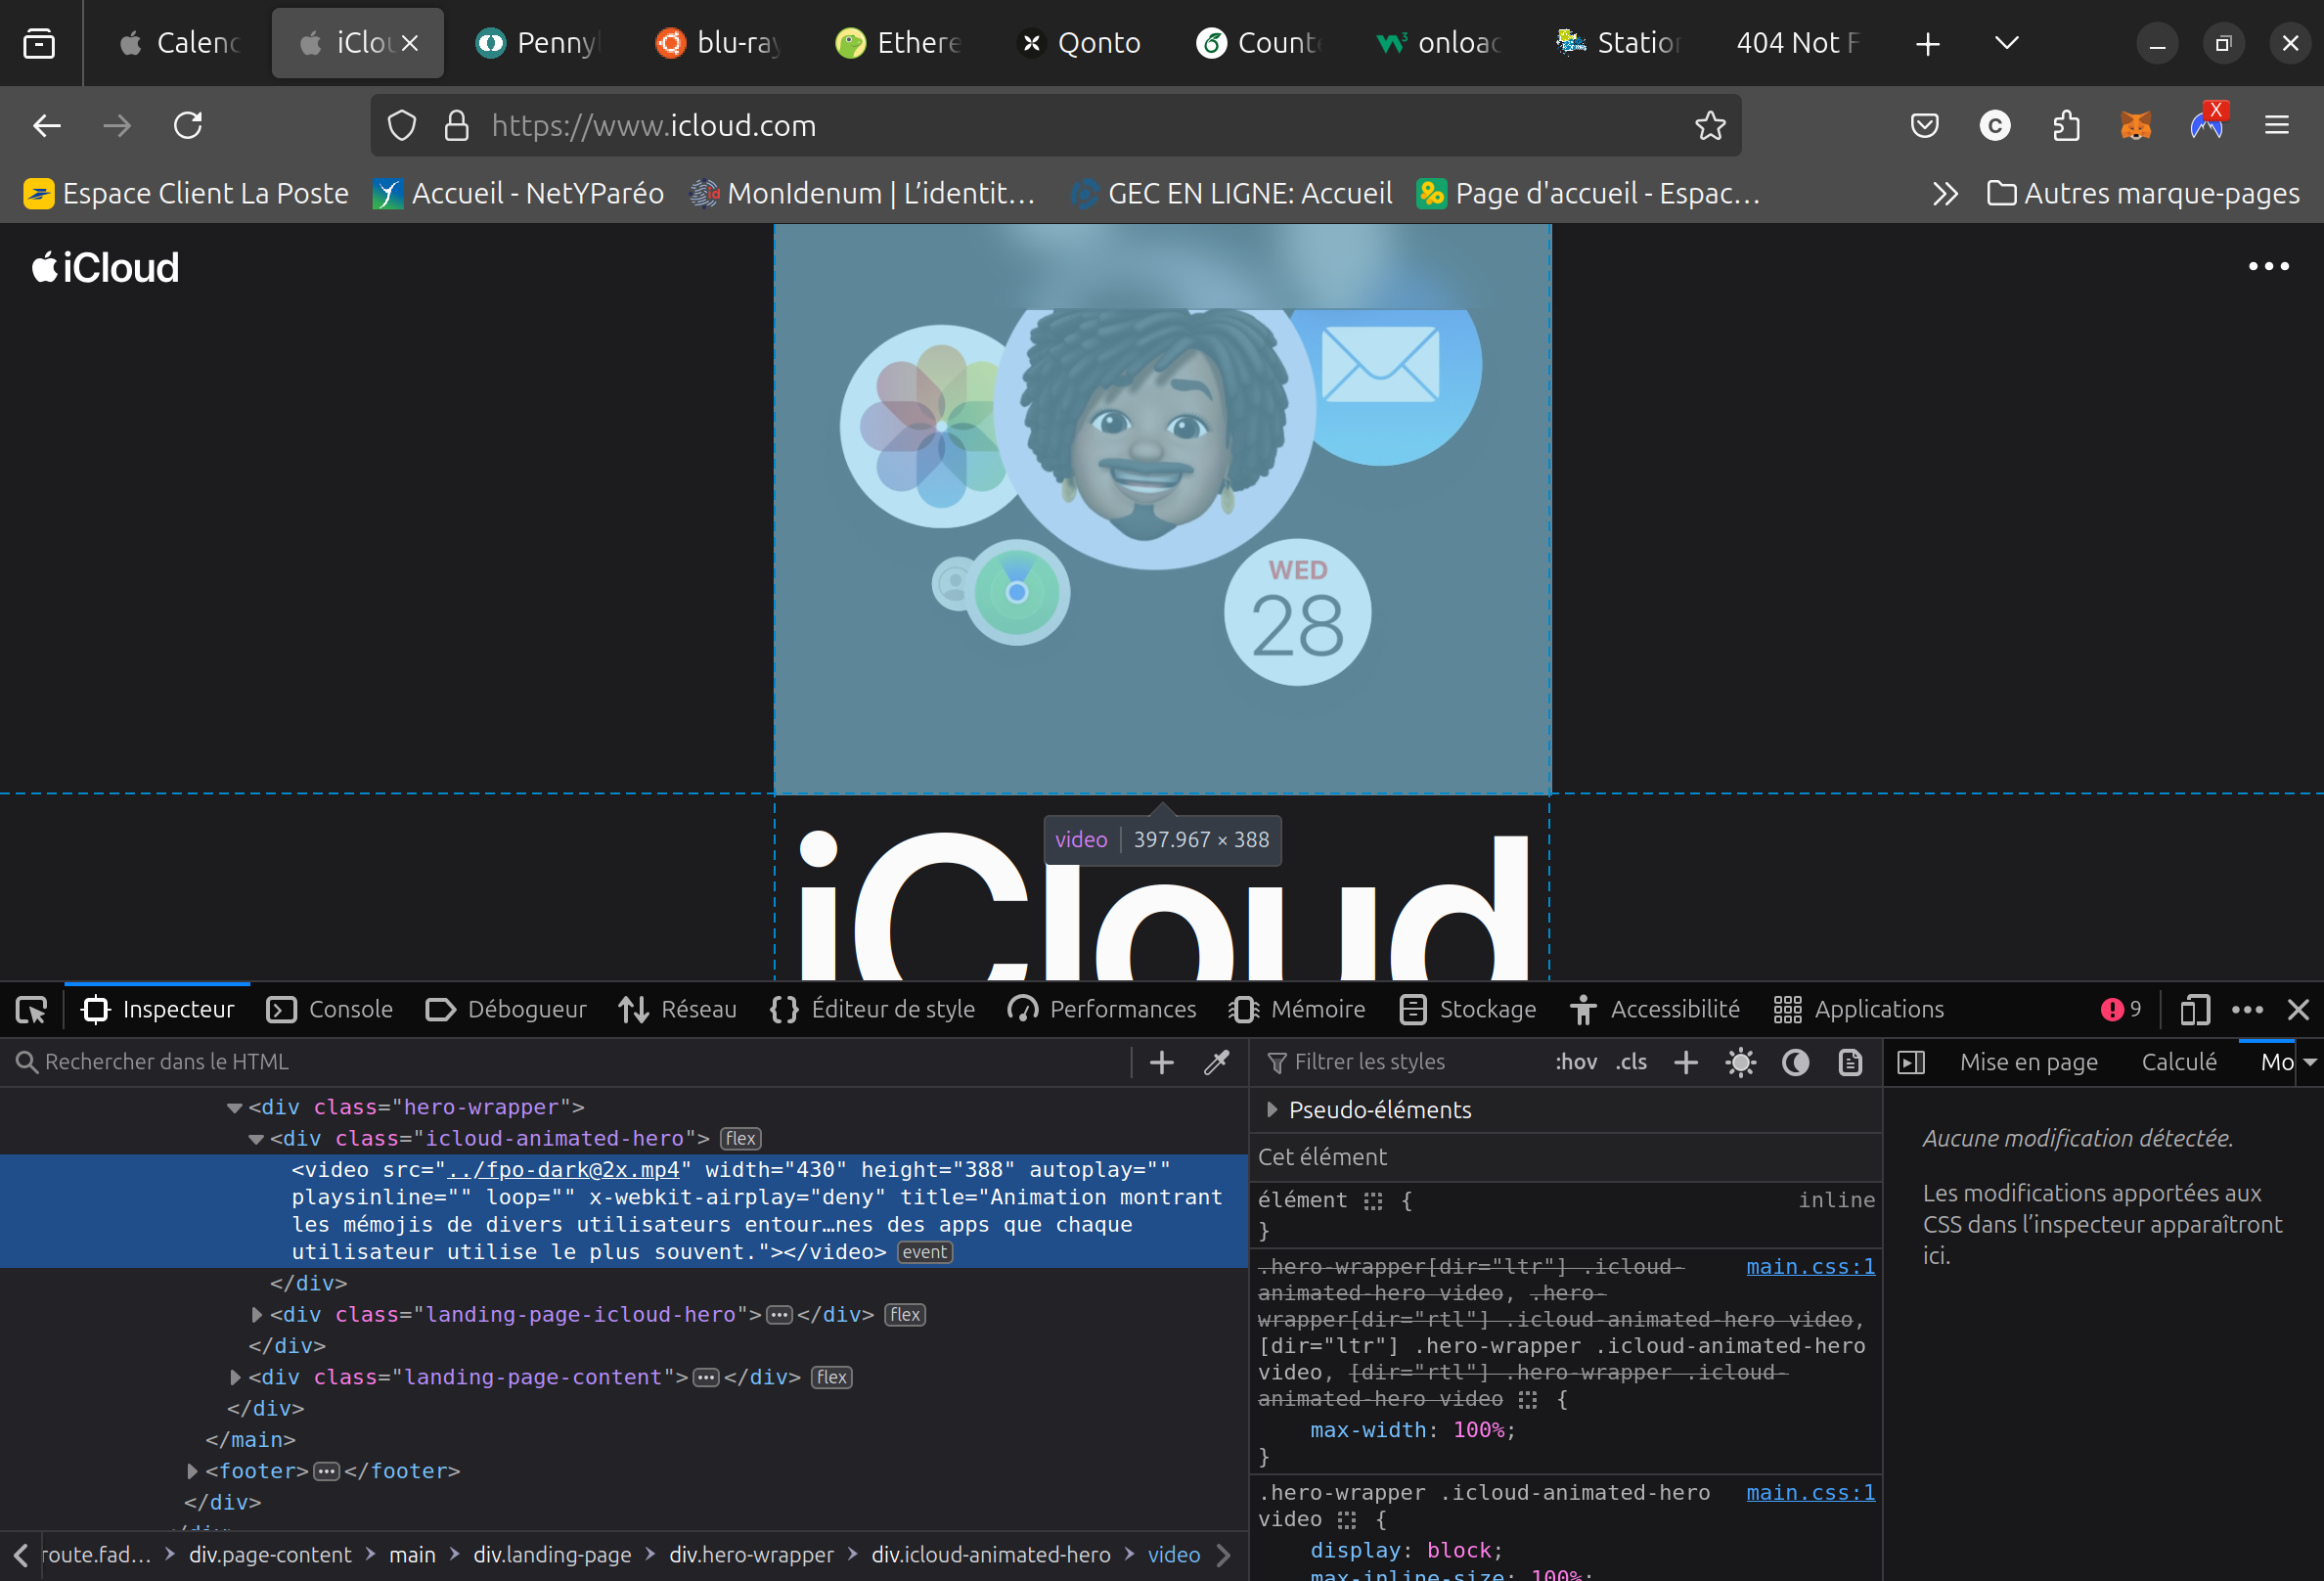
\includegraphics[width=7cm]{image/inspector-highlight}
    \end{frame}

    \begin{frame}{Les bases du débug}{Inspection du HTML}
        Exercice \execcounterdispinc{}~:
        \bigbreak
        \begin{itemize}
            \item Inspecter la page \url{https://www.icloud.com/calendar/}.
            \item Trouver la classe du texte \textit{Organisez votre temps avec Calendrier
            iCloud. Vos calendriers sont toujours à jour sur n’importe quel appareil et sur
            le Web.}.
            \item Trouver la police de caractère de cette classe.
            \item Modifier la police de caractère de cette classe pour \textit{Comic Sans MS} et
            vérifier la prise en compte de la modification.
        \end{itemize}
        \bigbreak
        \centering
        
\includegraphics[width=3cm]{image/intelligence}
    \end{frame}

    \begin{frame}{Les bases du débug}{La console}
        La console est dédiée au JS, elle permet d'écrire du JS ou d'appeler du JS déjà connu de la page.
        \bigbreak
        \centering
        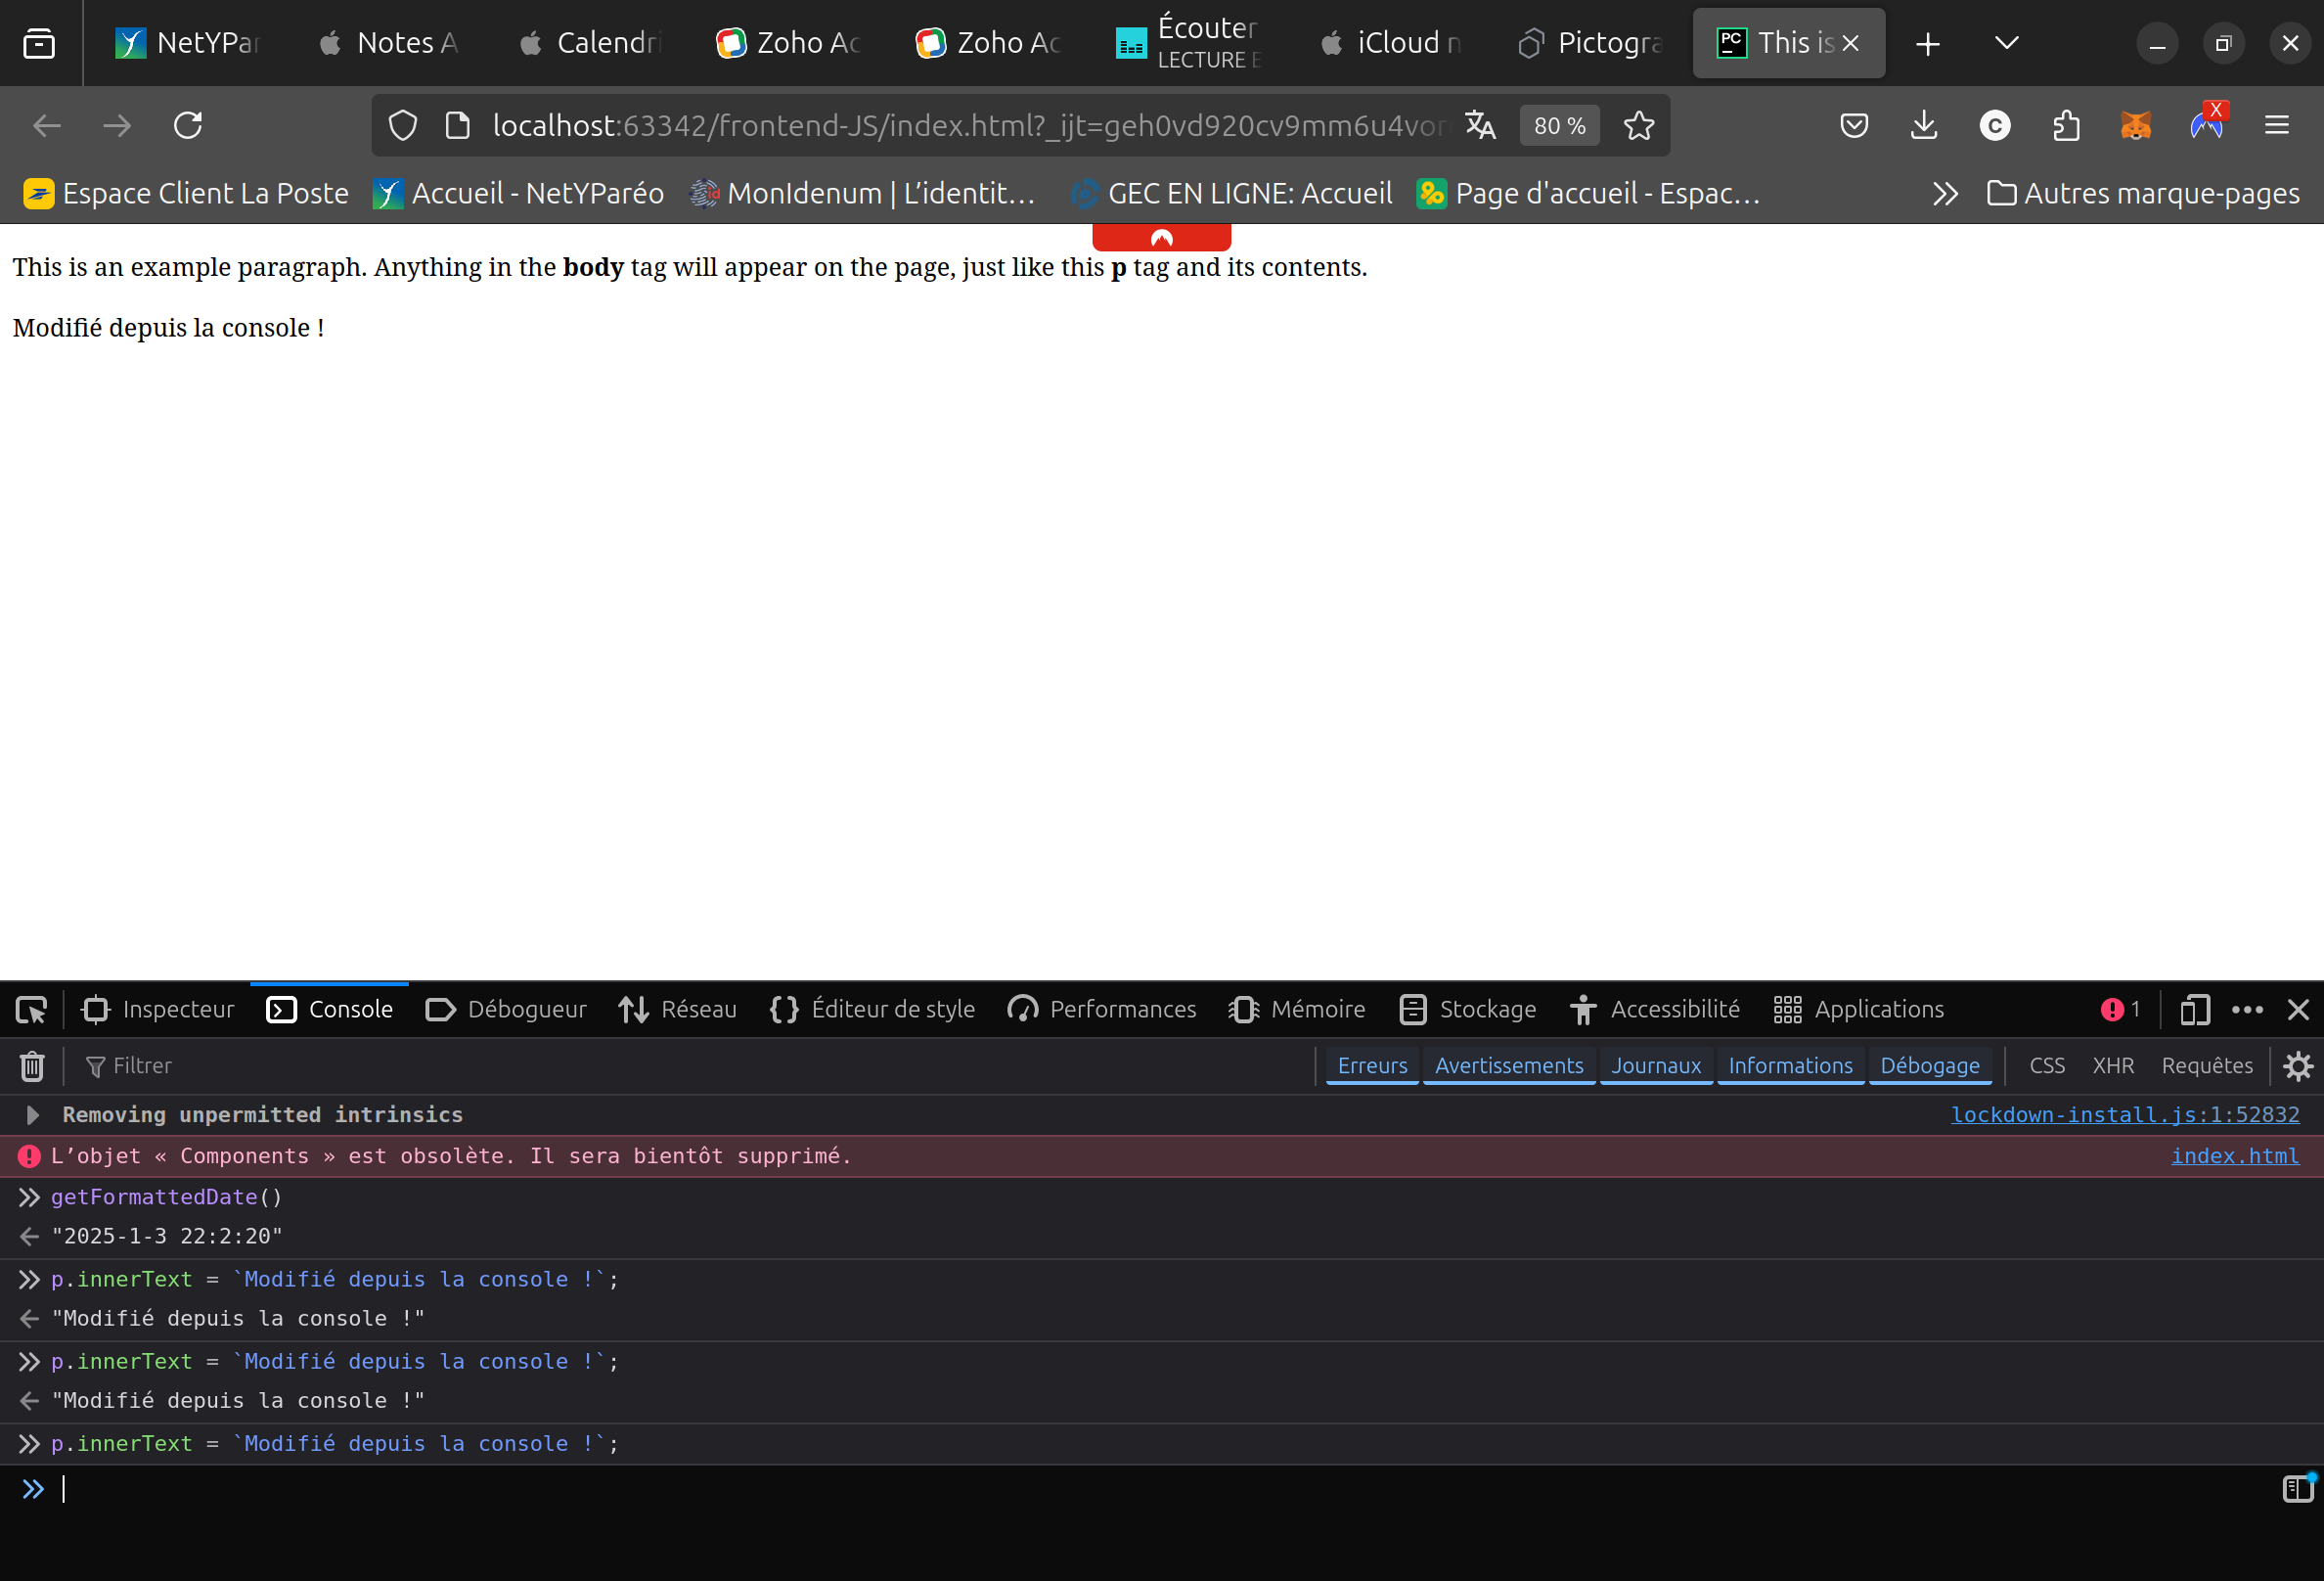
\includegraphics[width=8cm]{image/js-in-console}
        \bigbreak
        \flushleft
        Expliquer le comportement ci-dessus.
    \end{frame}

    \begin{frame}{Les bases du débug}{La console}
        Elle affiche (\textit{log}) les éventuels messages de warning, info, erreur lors de l'exécution et les erreurs de syntaxe.
        \bigbreak
        \centering
        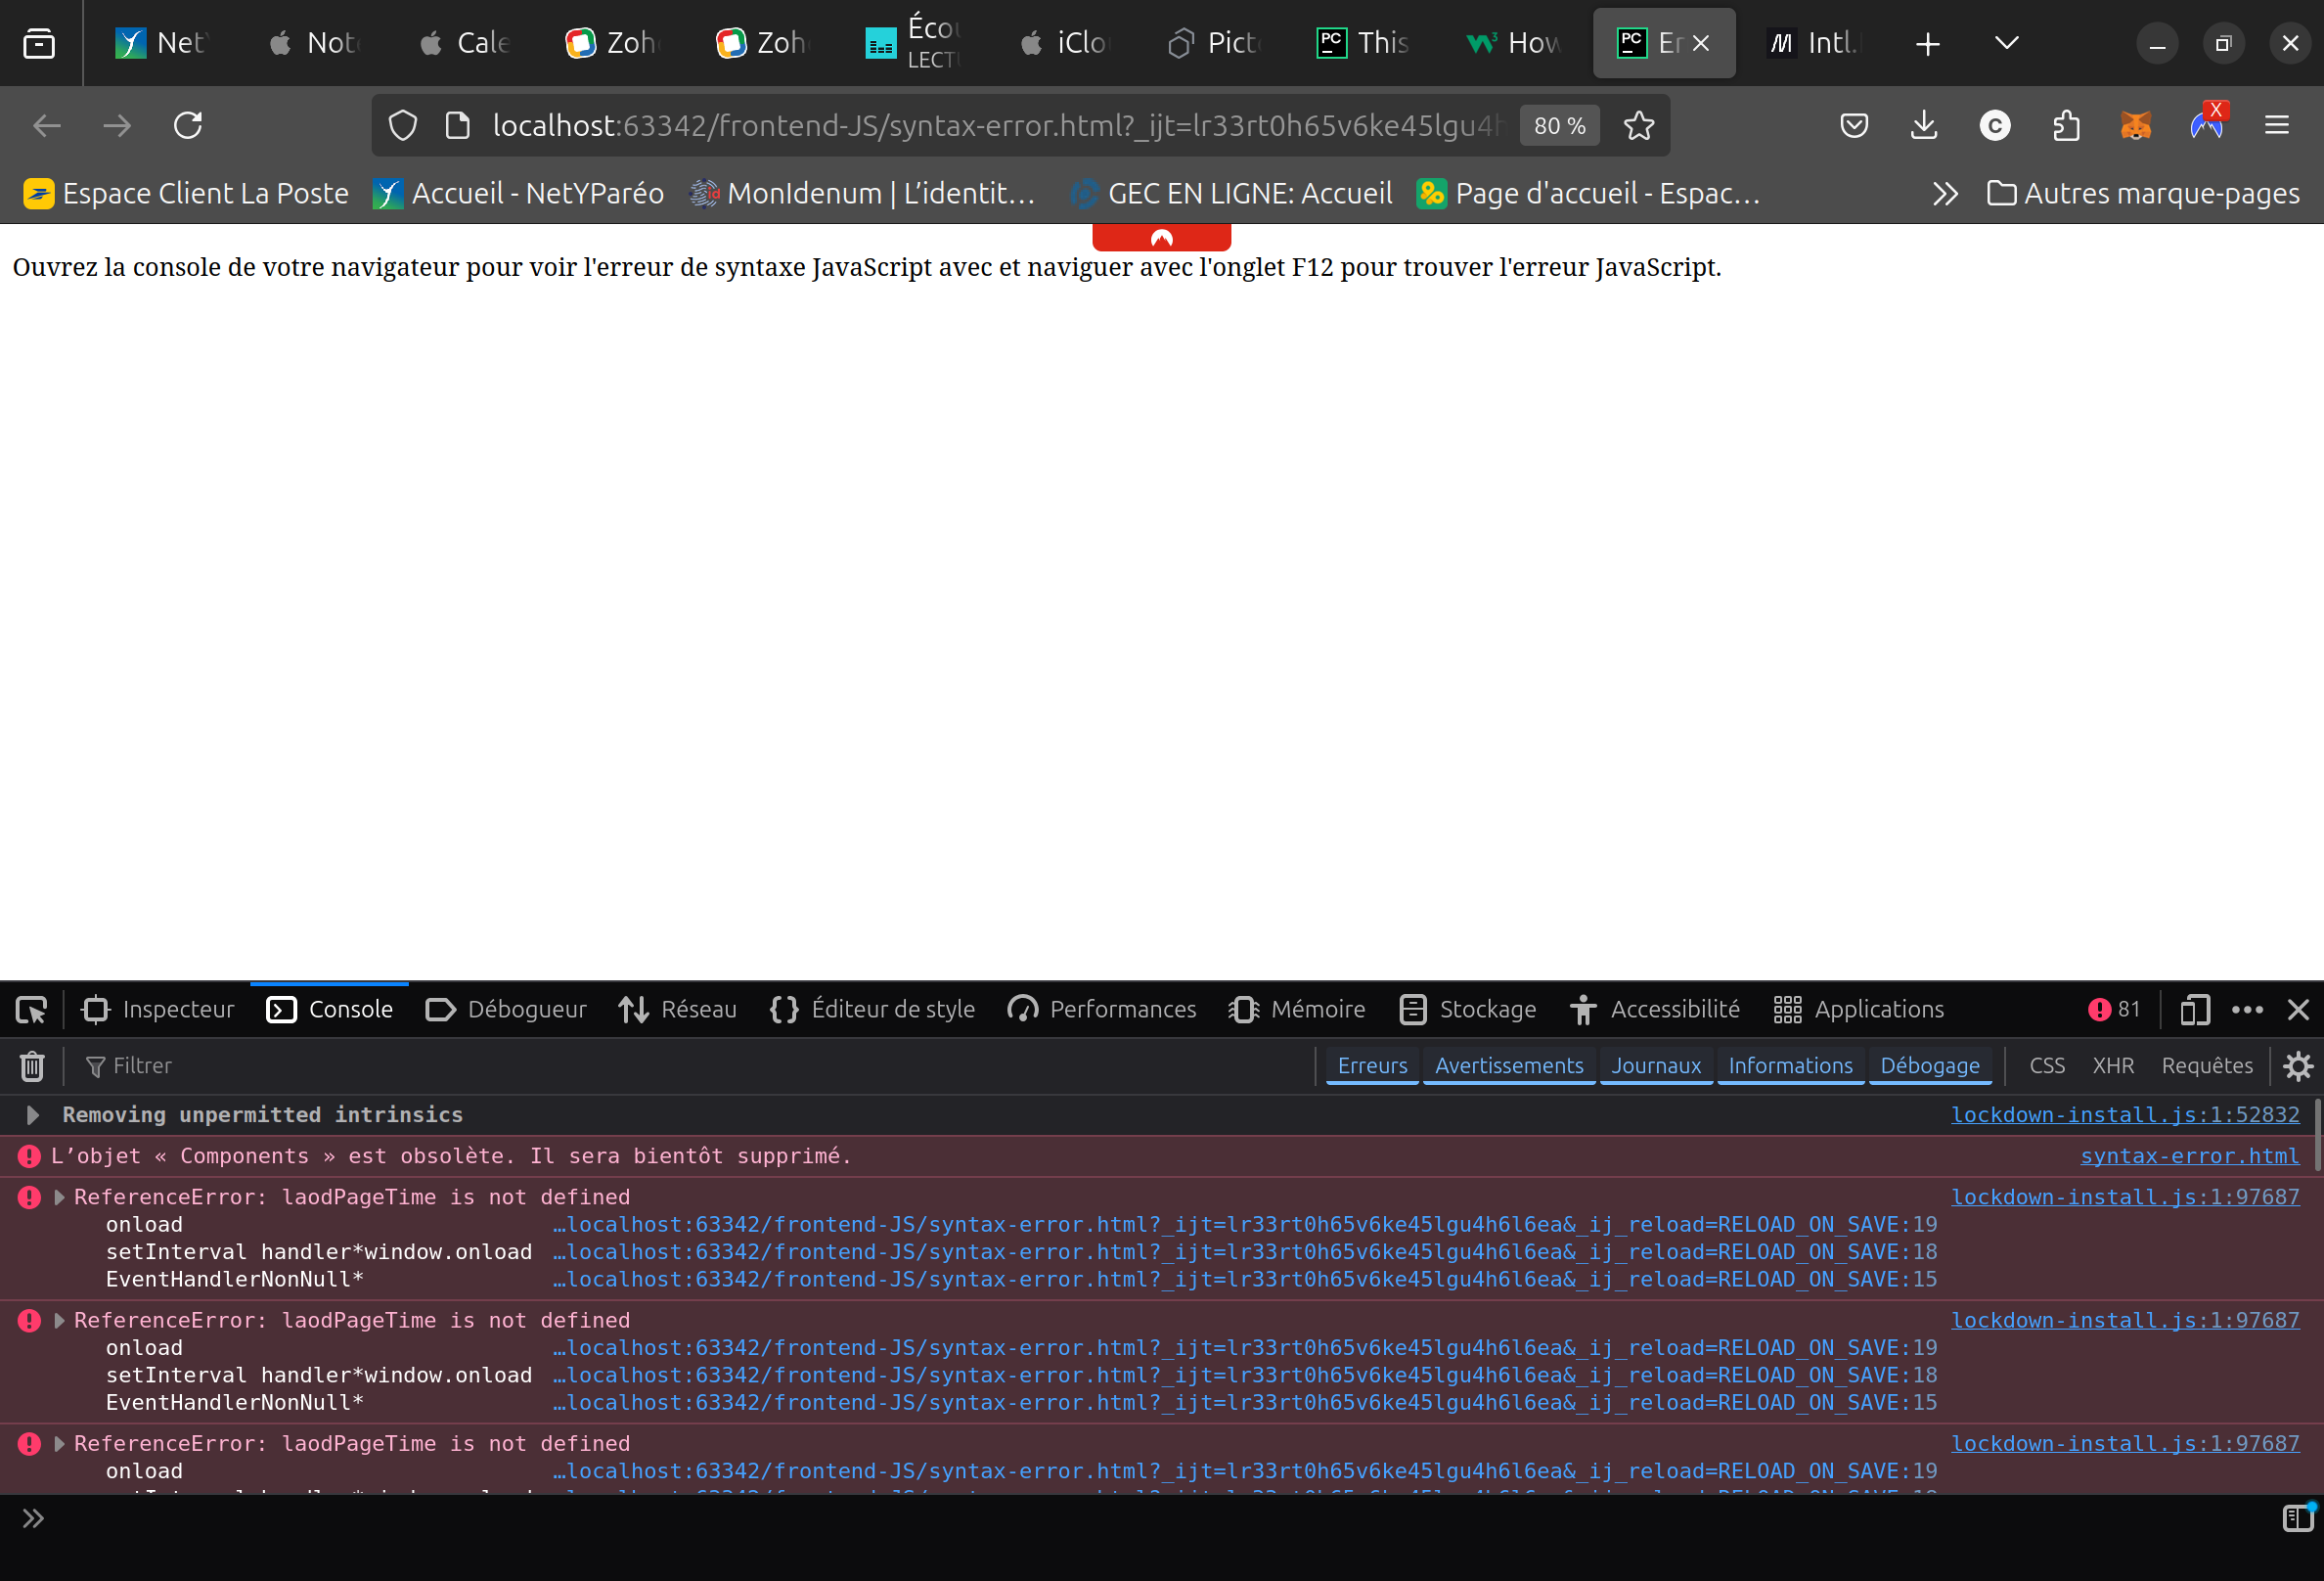
\includegraphics[width=7cm]{image/js-console-error-message}
        \flushleft
        On voit ici le parcours de l'interpréteur jusqu'à l'erreur en commençant par le dernier des appels.
    \end{frame}

    \begin{frame}{Les bases du débug}{La console}
        En cliquant sur le lien, on arrive sur le code source de l'erreur dans le débogueur.
        \bigbreak
        \centering
        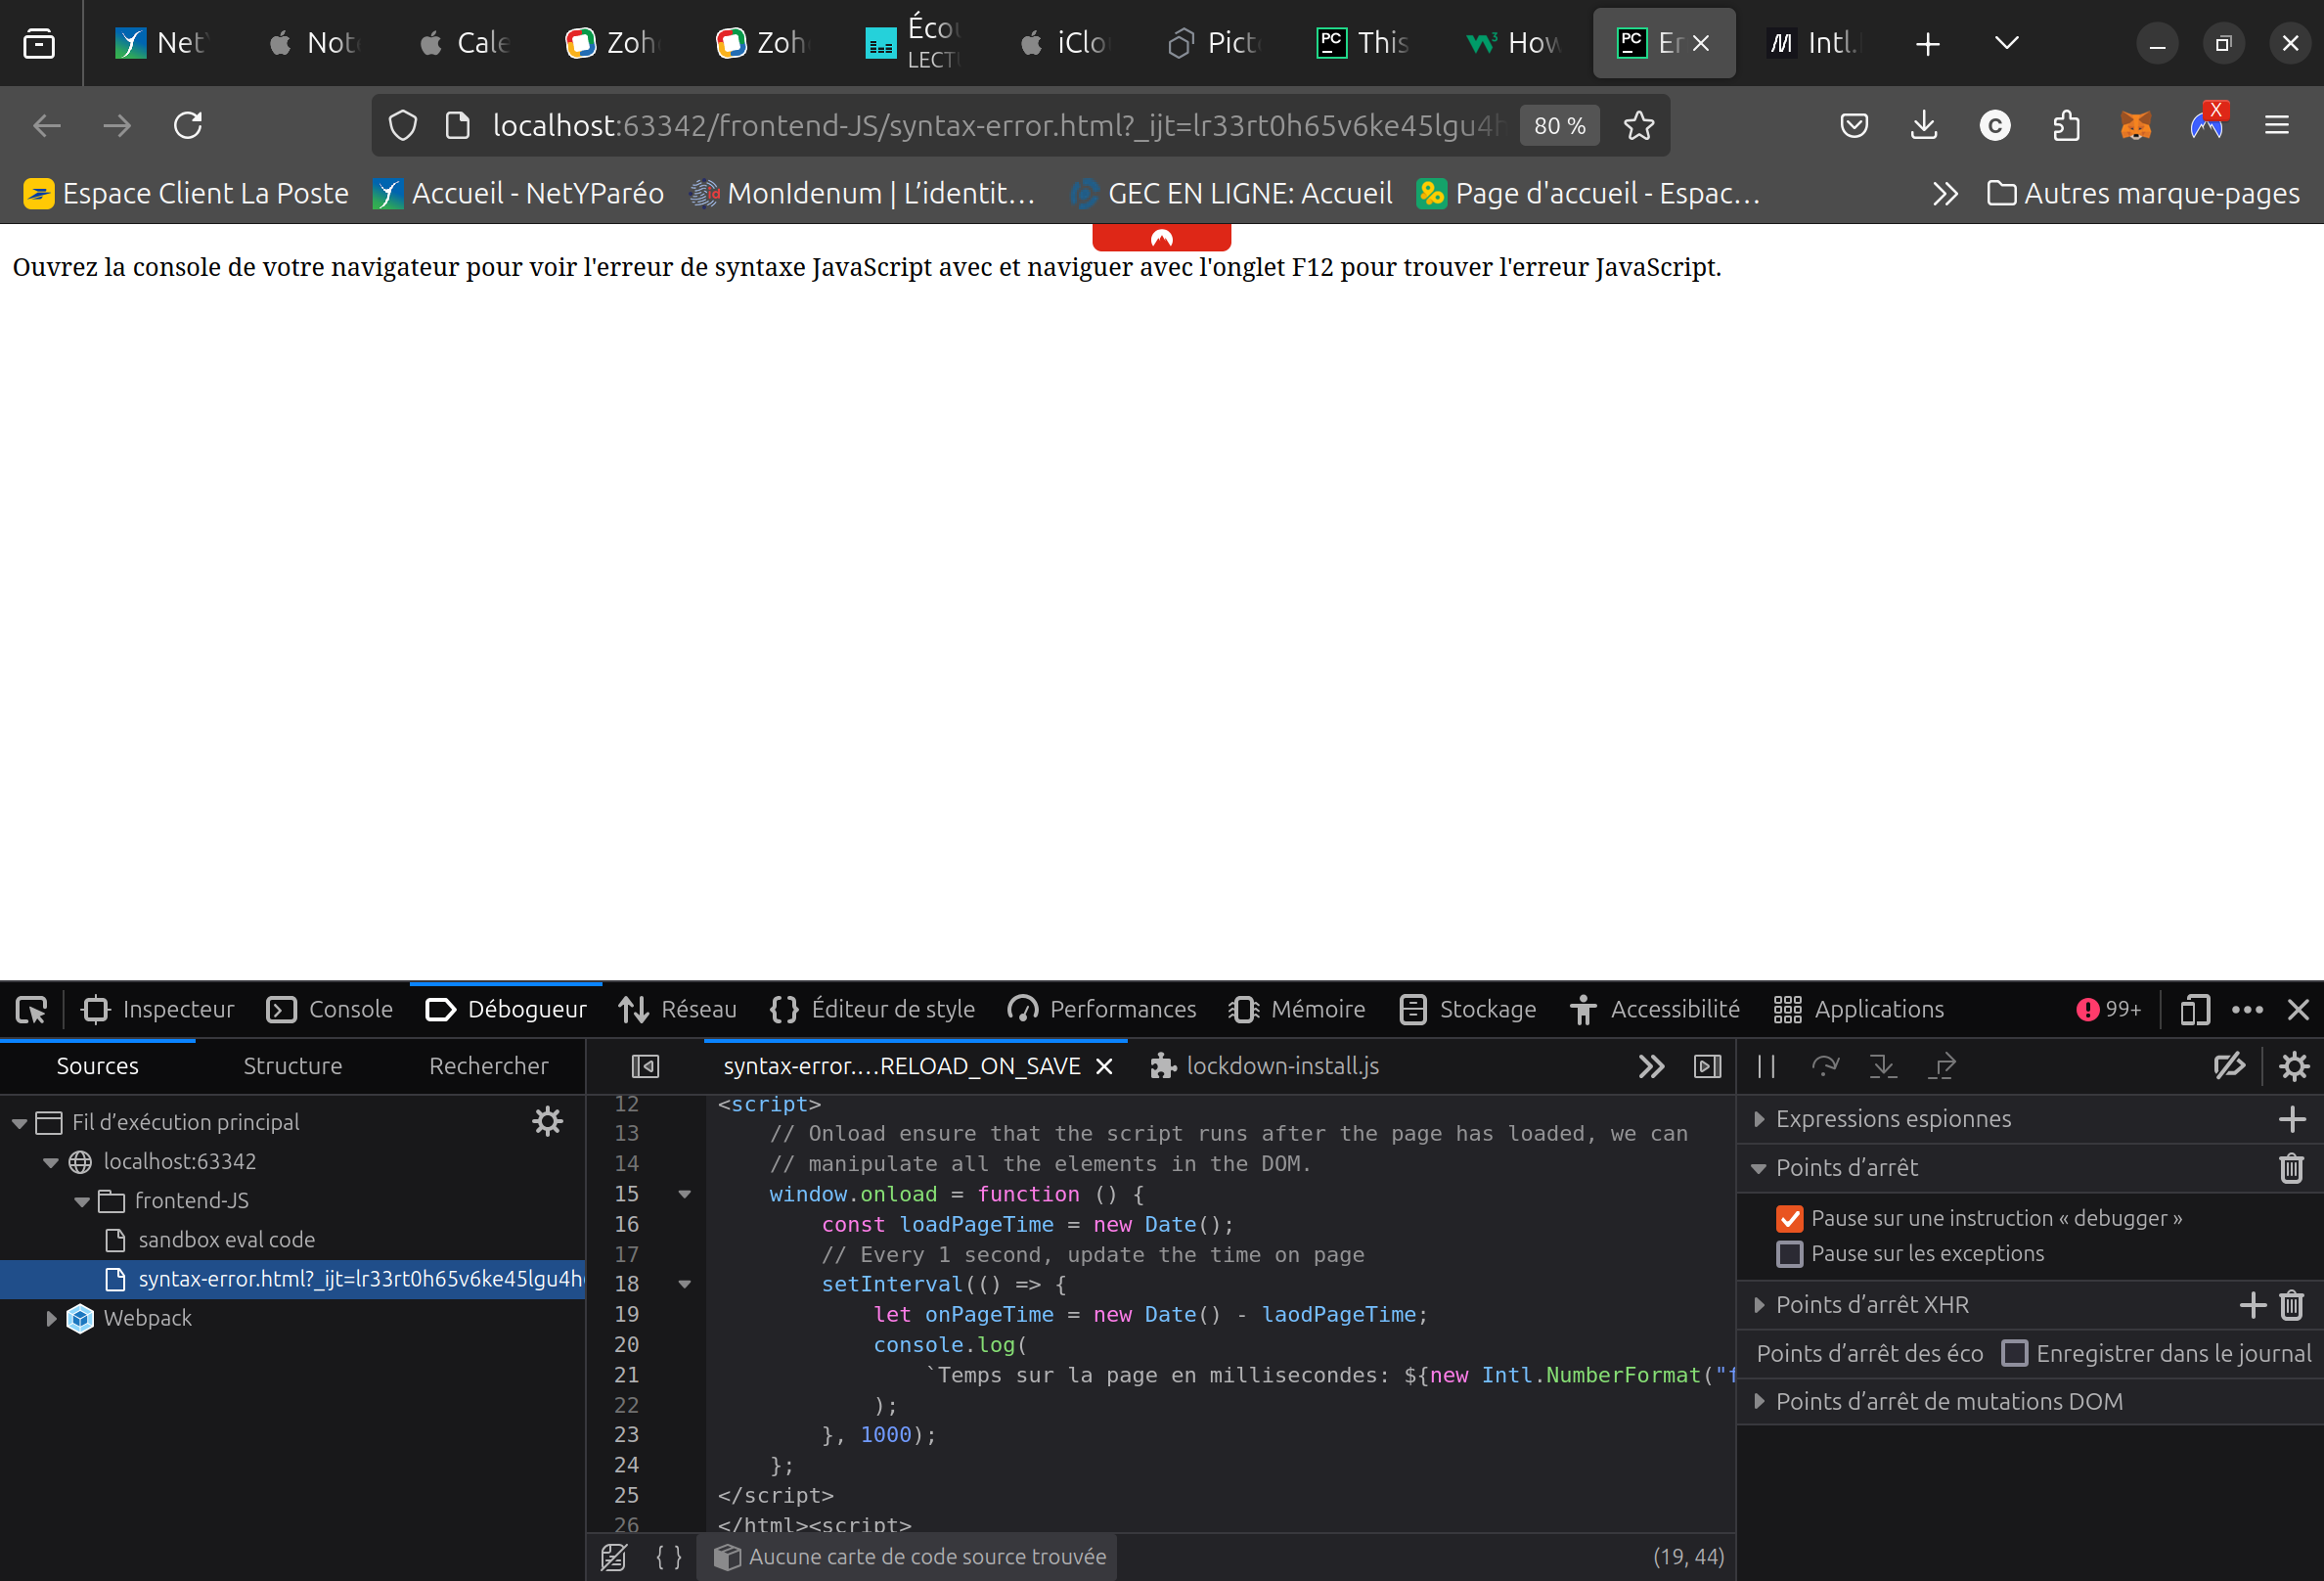
\includegraphics[width=9cm]{image/js-console-error-code}
    \end{frame}

    \begin{frame}{Les bases du débug}{Le débogueur}
        Le débogueur est, lui aussi, dédié au JS, il permet~:
        \begin{itemize}
            \item De lire le JS de la page.
            \item De mettre des points d'arrêt (\textit{breakpoints}) pour arrêter l'exécution du
            code.
            \item De naviguer dans le code, de pas en pas, de sauter des fonctions.
            \item De voir les valeurs des variables à un instant donné.
            \item De voir la pile d'appel des fonctions.
        \end{itemize}
    \end{frame}

    \begin{frame}{Les bases du débug}{Le débogueur}
        \bigbreak
        \centering
        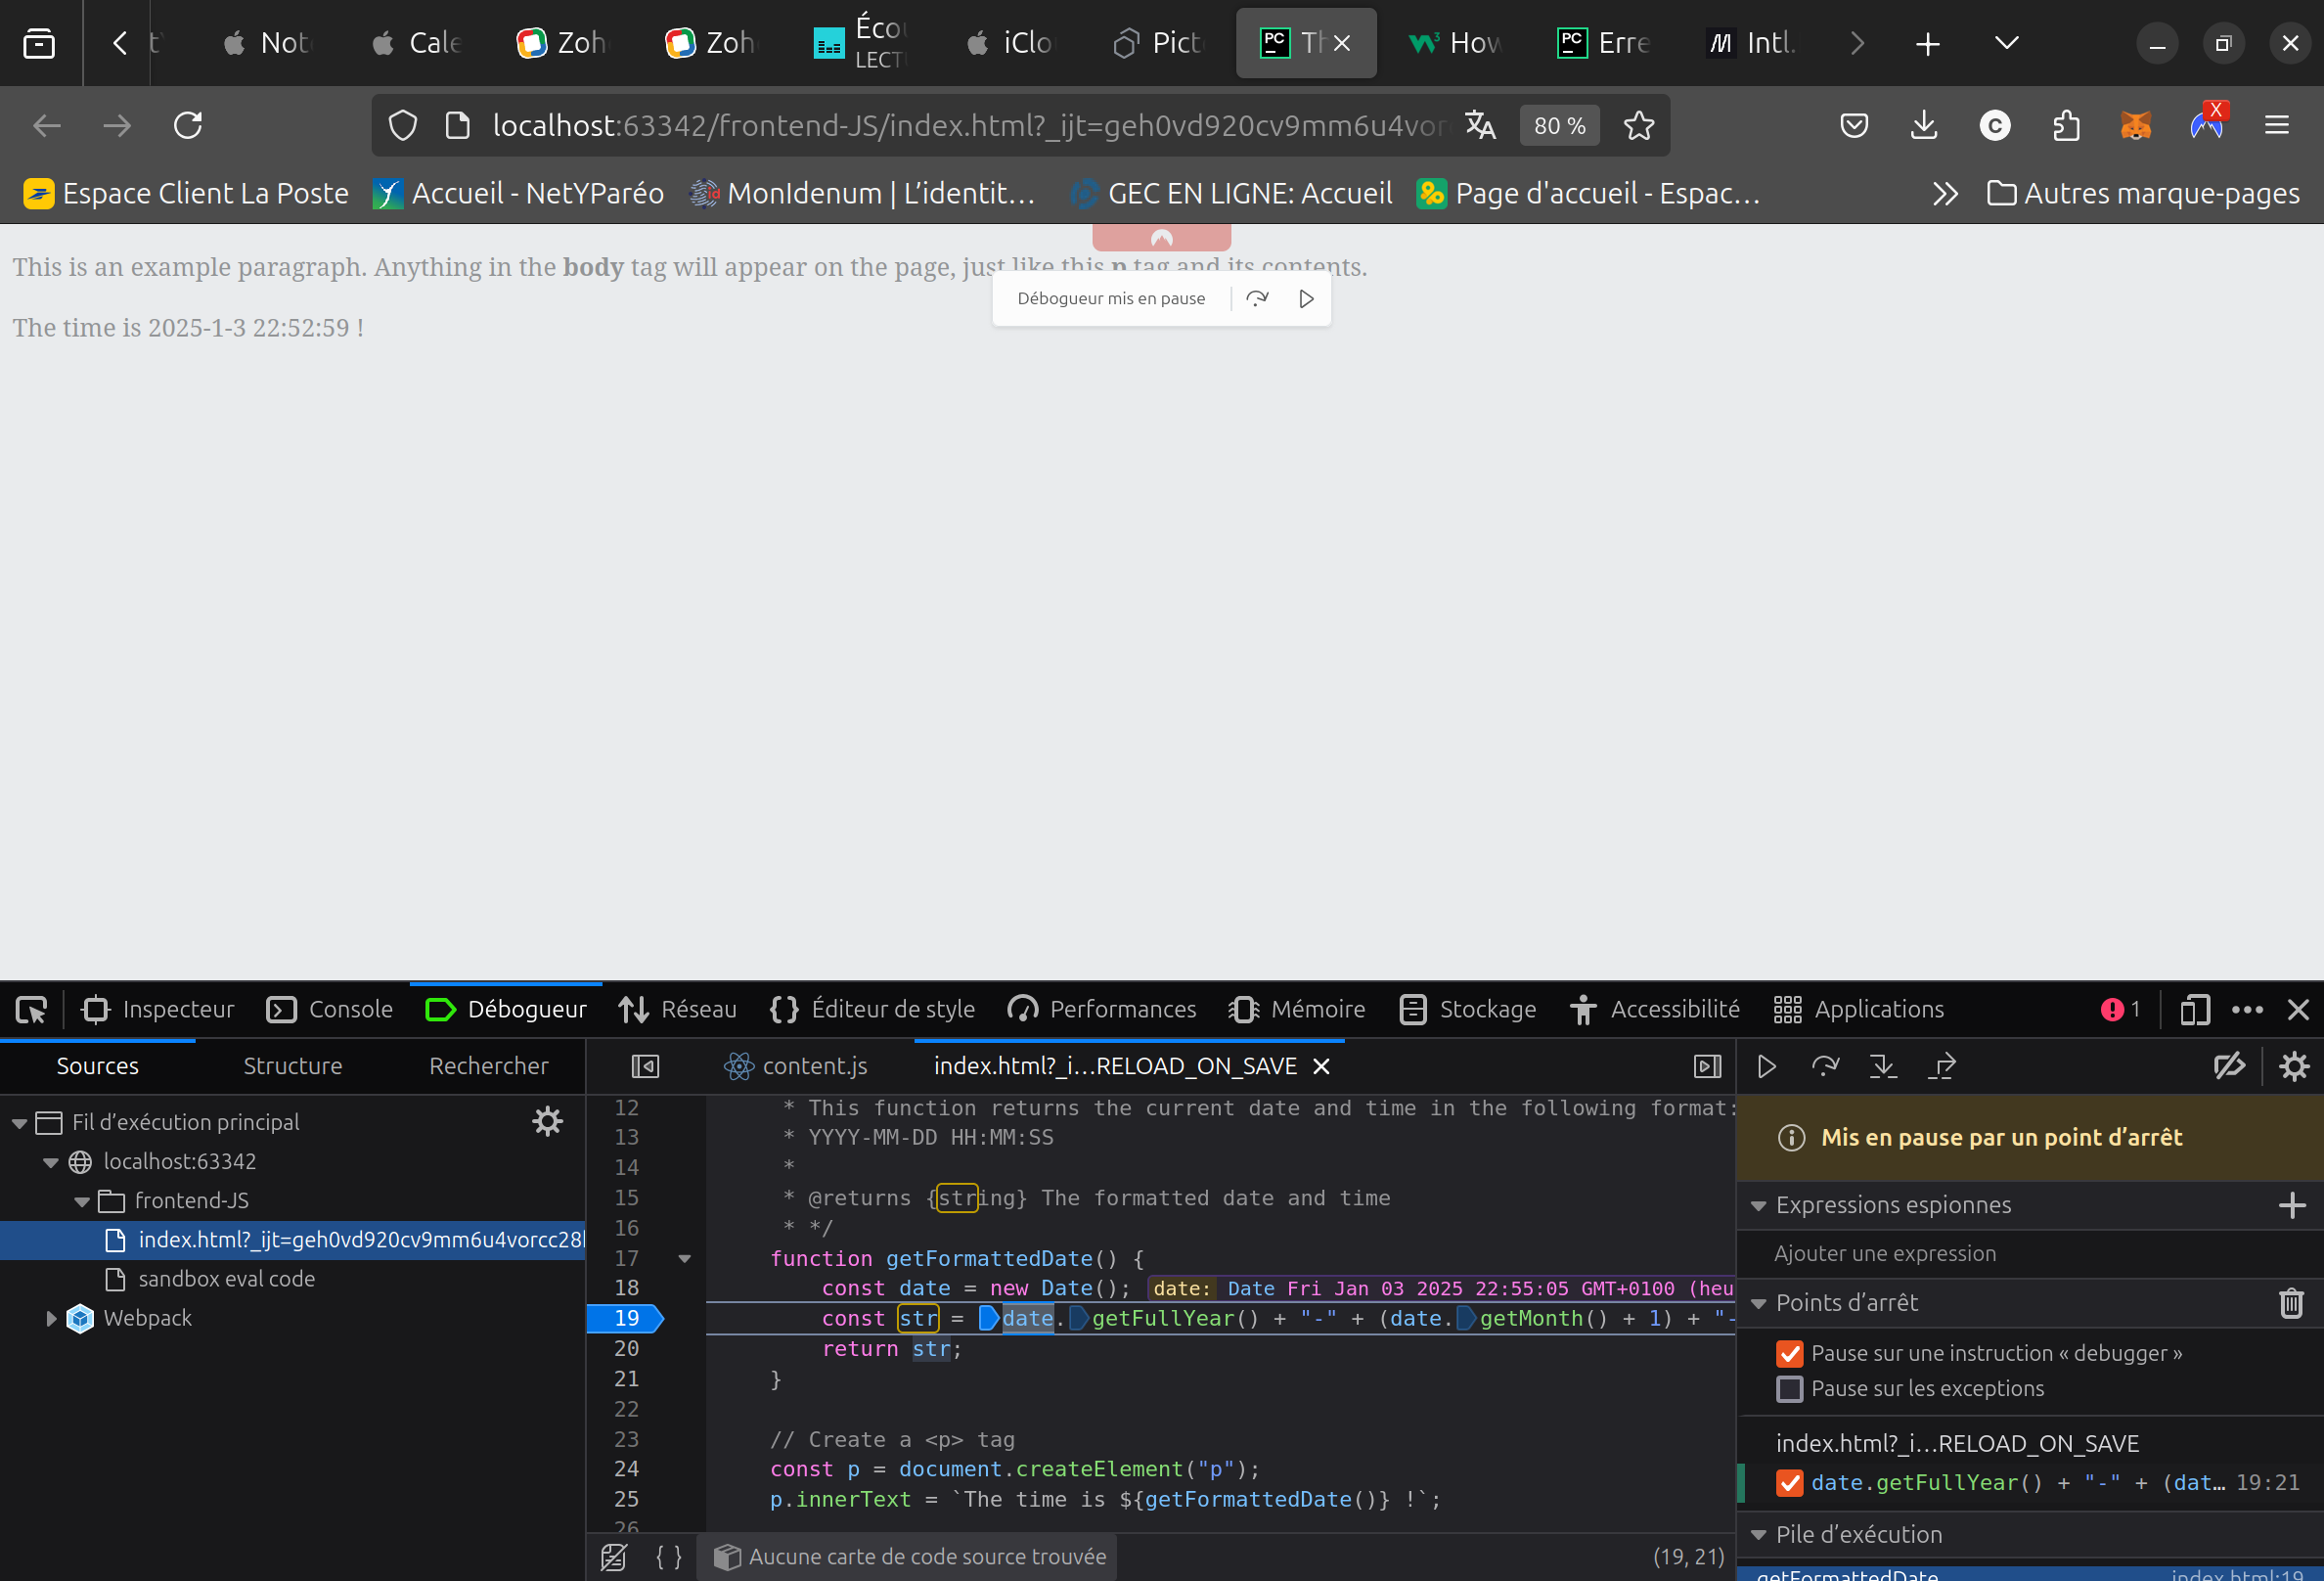
\includegraphics[width=10cm]{image/js-debugger}
    \end{frame}

    \begin{frame}{Les bases du débug}{Console et débogueur}
        Exercice \execcounterdispinc{}~:
        \begin{itemize}
            \item Naviguer à l'adresse \url{http://0.0.0.0/syntax-error.html}.
            \item Ouvrir la console.
            \item Cliquer sur le dernier appel pour aller au plantage
            \item Lire le code dans le débuggeur pour trouver l'erreur.
            \item Corriger l'erreur dans le code source et recharger la page.
        \end{itemize}
        \bigbreak
        \centering
        
\includegraphics[width=3cm]{image/intelligence}
    \end{frame}

    \begin{frame}{Les bases du débug}{Débogueur}
        Exercice \execcounterdispinc{}~:
        \begin{itemize}
            \item Naviguer à l'adresse \url{http://0.0.0.0/}.
            \item Ouvrir la débuggeur.
            \item Ajouter un point d'arrêt dans la fonction \lstinline{getFormattedDate}.
            \item Observer ce qui se passe.
            \item Faire du pas à pas pour comprendre le code.
        \end{itemize}
        \bigbreak
        \centering
        
\includegraphics[width=3cm]{image/intelligence}
    \end{frame}


    \section{Le langage JavaScript}\label{sec:js-lang}
    \begin{frame}{JavaScript}{L'historique\footnote{\label{mozilla-js}Une réintroduction à JavaScript, \url{https://developer.mozilla.org/fr/docs/Web/JavaScript/Language_overview}}}
        \begin{footnotesize}
            \begin{itemize}
                \item Créé en 1995 par Brendan Eich chez Netscape.
                \item En 1996, Java est très populaire et Netscape veut surfer sur la vague et
                renomme le langage appelé LiveScript en JavaScript.
                \item Standardisé par l'ECMA (European Computer Manufacturers Association) en 1997.
                \item Le standard est l'ECMAScript.
                \item La version actuelle implémentée dans les navigateurs se base sur le standard
                ES6 de 2015/2016.
                \item Les navigateurs implémentent des versions différentes de l'ES.
                \item JS est partout dans le backend ou programmation système avec Bun ou Node.js,
                pour le scripting de NoSQL comme CouchDB ou MongoDB, dans les PDF,
                \textit{etc}.
                \item Paradigme de programmation orienté objet mais s'adapte très bien au fonctionnel
                aussi et de mieux en mieux\ldots
            \end{itemize}
        \end{footnotesize}
    \end{frame}

    \begin{frame}{L'écosystème JavaScript}{Un langage interprété}
        \centering
        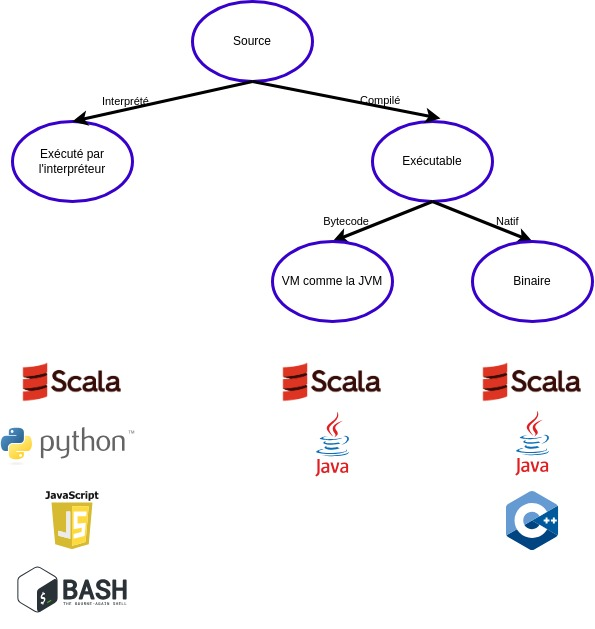
\includegraphics[width=7cm]{image/code-inter-vs-compiled}
    \end{frame}

    \begin{frame}{L'écosystème JavaScript}{Un langage interprété}
        \begin{small}
            De nombreux interpréteurs JavaScript existent dans les navigateurs, mais aussi en dehors~:
            \begin{itemize}
                \item \textbf{V8}, le moteur JavaScript de Chrome.
                \item \textbf{Node.js}, un interpréteur JavaScript côté serveur basé sur V8.
                \item \textbf{Deno}, un interpréteur JavaScript côté serveur basé sur V8, écrit en Rust par le développeur Node.js, il devrait lui succéder.
                \item \textbf{JavaScriptCore}, le moteur JavaScript de Safari.
                \item \textbf{SpiderMonkey}, le moteur JavaScript de Firefox.
                \item \textbf{Bun}, un environnement d'exécution plus rapide que Node.js et Deno\footnote{\label{bun}Bun is a fast JavaScript, \url{https://bun.sh/}}.
                \item \textbf{CouchDB}, une base de données NoSQL qui utilise JavaScript pour les requêtes dans sa version ES6 grâce à son binding avec SpiderMonkey, \footnote{The Road to CouchDB 3.0: Update to JavaScript Engine, \url{https://blog.couchdb.org/2020/02/26/the-road-to-couchdb-3-0-update-to-javascript-engine/}}.
                \item \textit{Many more}.
            \end{itemize}
        \end{small}
    \end{frame}

    \begin{frame}{L'écosystème JavaScript}{Les limites de notre cours}
        Sachant que ce cours s'appelle \textit{JavaScript Frontend}, dans quel(s) partie(s) de l'écosystème JavaScript allons-nous nous programmer~?
        \bigbreak
        \centering
        
\includegraphics[width=3cm]{image/intelligence}
        \pause
        \bigbreak
        \flushleft
        Nous allons programmer du JavaScript exécuté dans le navigateur, donc du JavaScript côté client.
    \end{frame}

    \begin{frame}{JavaScript dans le navigateur}{Les limites}
        Il existe de nombreuses limites à ce que peut faire le JavaScript dans le navigateur, principalement pour des raisons de sécurité~:
        \begin{itemize}
            \item Pas d'accès au système de fichiers, A.K.A. \textit{File System}, le disque dur.
            \item Capacités réseau limitées, seule une partie du protocole HTTP et le protocole
            WebSocket. Tout ce qui est protocole de bas niveau comme TCP, UDP, \textit{etc}
            est interdit. Il ne peut être que client, pas serveur.
            \item Le stockage de données se fait dans le navigateur, dans les cookies, le
            \textit{localStorage}, le \textit{sessionStorage} principalement.
            \item Pas d'accès à l'OS, donc pas de gestion de processus, tout est isolé dans le
            navigateur.
        \end{itemize}
    \end{frame}

    \begin{frame}{JavaScript dans le navigateur}{Les spécificités}
        \begin{scriptsize}
            Les spécificités du navigateur sont ses 2 A.P.I. (Application Programming Interface)~:
            \begin{itemize}
                \item Le DOM (Document Object Model)\footnote{Référence du DOM,
                    \url{https://developer.mozilla.org/fr/docs/Web/API/Document_Object_Model}}, qui
                permet de manipuler le contenu de la page dans les langages de balises HTML,
                XML, SVG.
                \item Le BOM (Browser Object Model)\footnote{Introduction au Browser Object Model
                    (BOM) et à l’objet Window,
                    \url{https://www.pierre-giraud.com/javascript-apprendre-coder-cours/browser-object-model-window/\#google_vignette}},
                qui permet de manipuler le navigateur et ses fenêtres (\lstinline{window})~:
                \begin{itemize}
                    \begin{scriptsize}
                        \item L’objet \lstinline{Navigator} qui représente l’état et l’identité du navigateur
                        et qu’on va utiliser avec l’API Geolocation.
                        \item L’objet \lstinline{History} qui permet de manipuler l’historique de navigation
                        du navigateur.
                        \item L’objet \lstinline{Location} qui fournit des informations relatives à l’URL de
                        la page courante.
                        \item L’objet \lstinline{Screen} qui nous permet d’examiner les propriétés de l’écran
                        qui affiche la fenêtre courante.
                        \item L’objet \lstinline{Document} et le DOM dans son ensemble que nous étudierons en
                        détail dans la suite.
                    \end{scriptsize}
                \end{itemize}
            \end{itemize}
        \end{scriptsize}
    \end{frame}

    \begin{frame}{JavaScript dans le navigateur\footnote{\label{eloquent-javaScript}Eloquent JavaScript, Marjin Haverbeke, \url{https://eloquentjavascript.net}}}{Les prérequis}
        Pour utiliser une API, quelle qu'elle soit, quel que soit le langage, il faut d'abord maîtriser les bases de ce dernier.
        \bigbreak
        Les bases de JS que nous allons couvrir ici sont les suivantes~:
        \begin{itemize}
            \item Les types
            \item La déclaration de variables
            \item Le scope des variables
            \item Les structures de contrôle (\textit{control flow})
            \item La déclaration de fonctions
            \item Les objets
            \item Les méthodes built-in
            \item Les exceptions
        \end{itemize}
    \end{frame}

    \subsection{Installation de WebStorm}\label{subsec:installwebstorm}

    \begin{frame}{Développement d'un script}{Installation d'un IDE}
        \begin{small}
            Un IDE est un \textit{Integrated Development Environment}, un environnement de développement intégré, logiciel d'édition de texte dédié à la programmation.
            \bigbreak
            Les principaux environnements de développement en JS sont VS Code de Microsoft et WebStorm de JetBrains.

            WebStorm est gratuit pour les étudiants, vous pouvez avoir une licence en
            créant un compte avec votre adresse MDS~. \bigbreak Installer également Node.js
            pour avoir un REPL (Read, Evaluate, Print and Loop)
        \end{small}
        \bigbreak
        \centering
        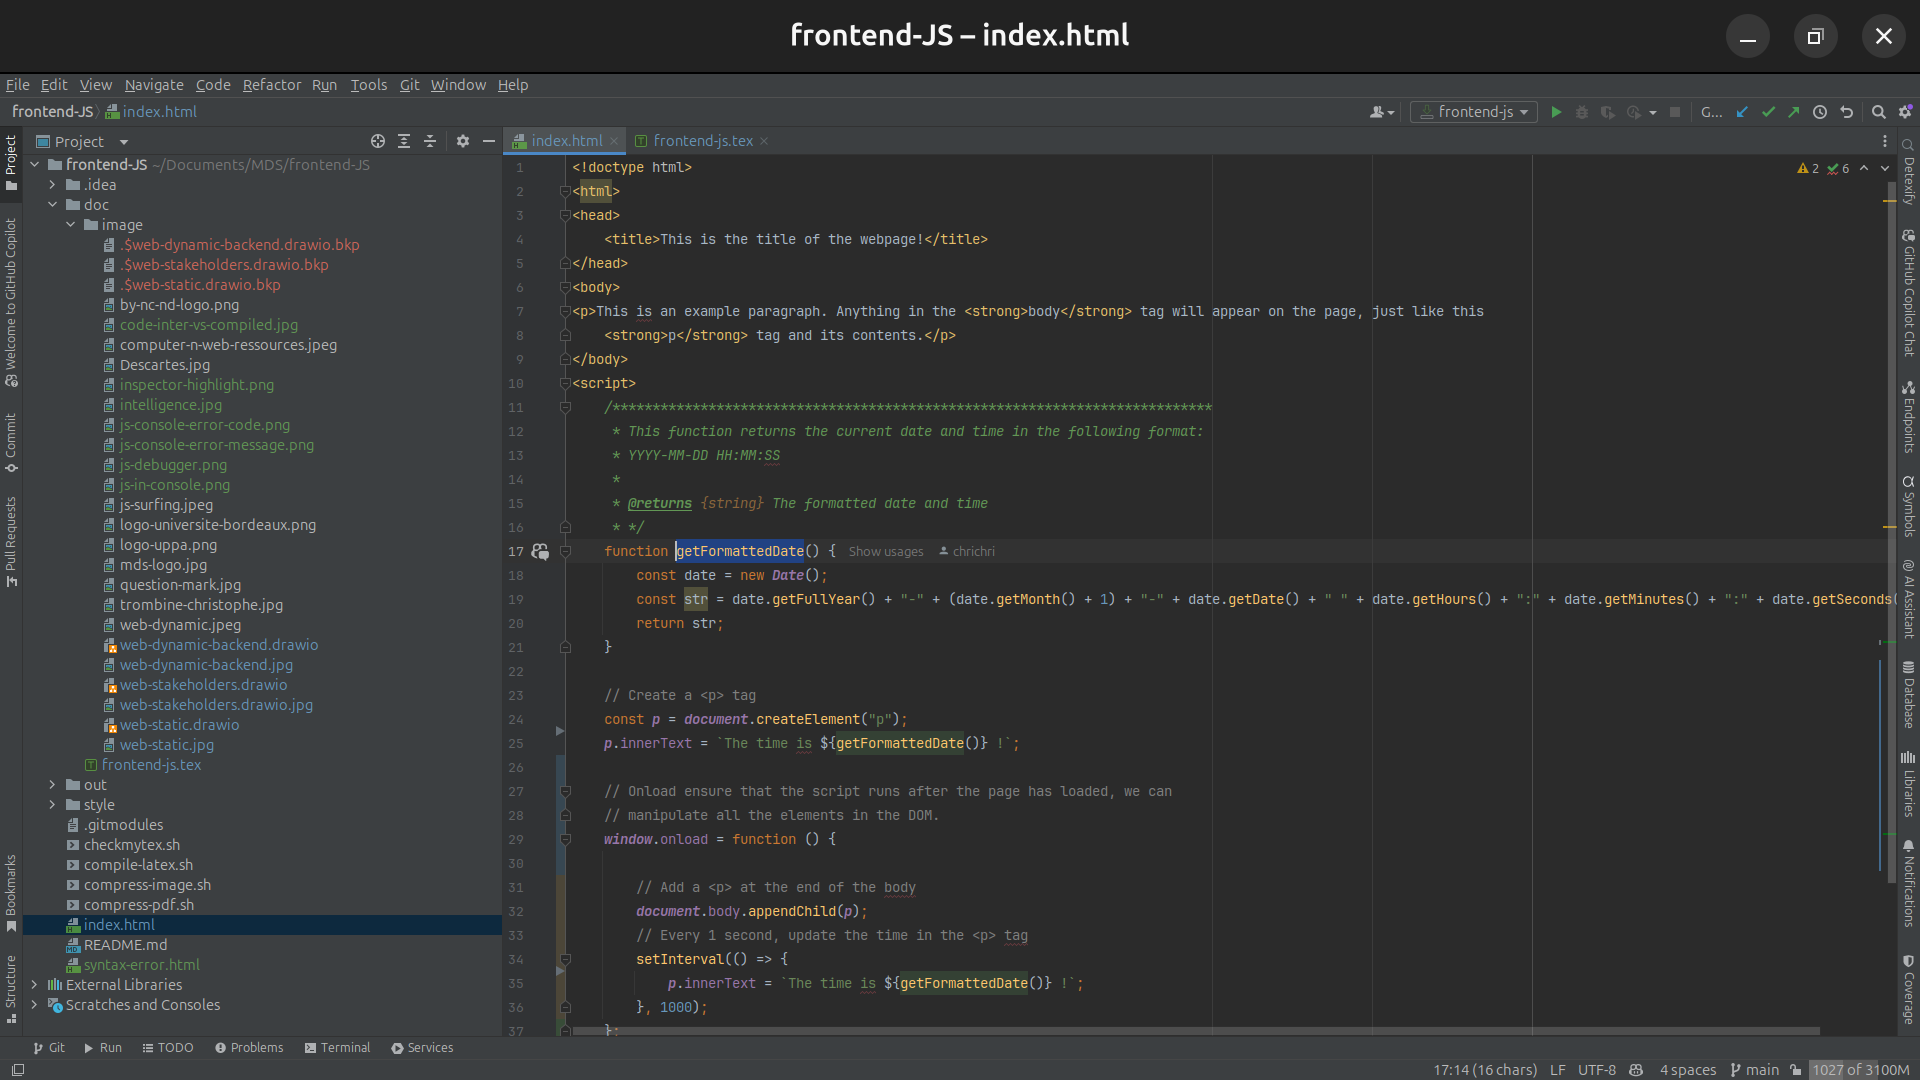
\includegraphics[width=6cm]{image/webstorm}
    \end{frame}

    \subsection{Initialisation du projet}\label{subsec:projectinit}

    \begin{frame}{Développement d'un script}{Mon premier script}
        \begin{itemize}
            \item Télécharger le code de ce cours sur GitHub
            \url{https://github.com/My-Digital-School-by-PapIT/frontend-JS}.
            \item Dézipper l'archive.
            \item Ouvrir le dossier avec WebStorm.
            \item Créer un fichier avec une extension
            \lstinline{js} comme \lstinline{variables-n-types.js} par exemple.
        \end{itemize}
        \bigbreak
        \centering
        
\includegraphics[width=3cm]{image/intelligence}
    \end{frame}

    \subsection{Déclarations et types primitifs}\label{subsec:declare-n-types}

    \begin{frame}[fragile]{Déclarations et types}{Les types numériques}
        \begin{lstlisting}[language=JavaScript,title={\tiny{Script JavaScript}},basicstyle=\tiny\ttfamily]
// Ceci est un commentaire et ne sera pas exécuté
/*
Ceci est un commentaire multiligne et ne sera pas exécuté
*/

/*
Déclaration de variable numérique, elle a un scope avec var, un nom myAge et une
valeur à 39 dont le type est "inféré" par le langage, ici un type Number.
Toutes les déclarations se terminent par un ; par convention, il est optionnel.
*/
var myAge = 39; // 39 est un nombre entier (integer en anglais)
// Console.log est une fonction qui permet d'afficher des messages dans la console
console.log("J'ai " + myAge + " ans");
// Affiche le type de la variable myAge que l'on récupère avec l'opérateur typeof
console.log("Le type de la variable myAge qui n'a été déclaré (le type) est " + typeof myAge);

var myHeight = 1.85; // 1.75 est un nombre réel (float en anglais)
console.log("Je mesure " + myHeight + " mètre"); console.log("Le type de la variable myHeight qui n'a été déclaré (le type) est " + typeof myHeight);
// Les deux nombres entiers et réels sont de type Number en JavaScript.
        \end{lstlisting}
    \end{frame}

    \begin{frame}[fragile]{Déclarations et types}{Les types numériques}
        \begin{lstlisting}[language=JavaScript,title={\tiny{Script JavaScript}},basicstyle=\tiny\ttfamily]
// Mais peut aussi être déclaré de manière explicite
var myAge = Number(39); // 39 est un nombre entier (integer en anglais)
// Console.log est une fonction qui permet d'afficher des messages dans la console
console.log("J'ai " + myAge + " ans");
// Affiche le type de la variable myAge que l'on récupère avec l'opérateur typeof
console.log("Le type de la variable myAge qui n'a été déclaré (le type) est " + typeof myAge);
var myHeight = Number(1.85); // 1.75 est un nombre réel (float en anglais)
console.log("Je mesure " + myHeight + " mètre");
console.log("Le type de la variable myHeight qui n'a été déclaré (le type) est " + typeof myHeight);
        \end{lstlisting}
    \end{frame}

    \begin{frame}[fragile]{Déclarations et types}{Les grands entiers}
        \begin{lstlisting}[language=JavaScript,title={\tiny{Script JavaScript}},basicstyle=\tiny\ttfamily]
/* Mais pour l'arithmétique des grands nombres, il est préférable d'utiliser BigInt.
Ils sont à utiliser au-dessus du nombre définit dans Number.MAX_SAFE_INTEGER
qui peut varier en fonction des machines
*/
console.log("Le nombre maximum de Number est " + Number.MAX_SAFE_INTEGER);
var myBigNumber = BigInt(Number.MAX_SAFE_INTEGER) + BigInt(1);
console.log("Le type de la variable myBigNumber qui n'a été déclaré (le type) est " + typeof myBigNumber);
        \end{lstlisting}
        \begin{dangercolorbox}
            Mais BigInt ne fonctionne que pour les entiers, pas les réels.
        \end{dangercolorbox}
        \begin{lstlisting}[language=Bash,title={\tiny{Node.js}}]
> var myBigNumber = BigInt(Number.MAX_SAFE_INTEGER) + BigInt(1.666);
Uncaught:
RangeError: The number 1.666 cannot be converted to a BigInt because it is not an integer
at BigInt (<anonymous>)
> var myBigNumber = BigInt(Number.MAX_SAFE_INTEGER) + 1.666;
Uncaught TypeError: Cannot mix BigInt and other types, use explicit conversions
        \end{lstlisting}
    \end{frame}

    \begin{frame}[fragile]{Déclarations et types}{Les grands entiers}
        \begin{lstlisting}[language=JavaScript,title={\tiny{Script JavaScript}},basicstyle=\tiny\ttfamily]
/* Mais pour l'arithmétique des grands nombres, il est préférable d'utiliser BigInt.
Ils sont à utiliser au-dessus du nombre définit dans Number.MAX_SAFE_INTEGER
qui peut varier en fonction des machines
*/
console.log("Le nombre maximum de Number est " + Number.MAX_SAFE_INTEGER);
var myBigNumber = BigInt(Number.MAX_SAFE_INTEGER) + BigInt(1);
console.log("Le type de la variable myBigNumber qui n'a été déclaré (le type) est " + typeof myBigNumber);
        \end{lstlisting}
        \begin{dangercolorbox}
            Mais BigInt ne fonctionne que pour les entiers, pas les réels.
        \end{dangercolorbox}
        \begin{lstlisting}[language=Bash,title={\tiny{Node.js}},basicstyle=\tiny\ttfamily]
> var myBigNumber = BigInt(Number.MAX_SAFE_INTEGER) + BigInt(1.666);
Uncaught:
RangeError: The number 1.666 cannot be converted to a BigInt because it is not an integer
at BigInt (<anonymous>)
> var myBigNumber = BigInt(Number.MAX_SAFE_INTEGER) + 1.666;
Uncaught TypeError: Cannot mix BigInt and other types, use explicit conversions
        \end{lstlisting}
    \end{frame}

    \begin{frame}[fragile]{Déclarations et types}{Les grands entiers}
        On peut aussi déclarer un grand nombre en le suffixant avec un \lstinline{n} pour le forcer à être un BigInt.
        \begin{lstlisting}[language=Bash,title={\tiny{Node.js}}]
> atomNumber = 9999999999999999999999999999999999999999n
9999999999999999999999999999999999999999n
> typeof ato
Atomics atob atomNumber

> typeof atomNumber
'bigint'
        \end{lstlisting}
    \end{frame}

    \begin{frame}[fragile]{Déclarations et types}{Les nombres speciaux}
        Un nombre particulier existe en JS c'est \textit{Infinity} qui représente l'infini.
        \begin{lstlisting}[language=JavaScript,title={\tiny{Script JavaScript}}]
// Le nombre spécial Infinty
console.log("Le type de la variable Infinity qui n'a été déclaré (le type) est " + typeof Infinity);
console.log("Infinity - Infinity = " + Infinity - Infinity);
console.log("Infinity / 999999999999999999 = " + Infinity / 999999999999999999);
console.log("999999999999999999 / Infinity = " + 999999999999999999 / Infinity);
        \end{lstlisting}
    \end{frame}

    \begin{frame}[fragile]{Déclarations et types}{Les chaines de caractères}
        \begin{lstlisting}[language=JavaScript,title={\tiny{Script JavaScript}}]
/*
Déclaration d'une variable de type chaîne de caractère (string en anglais),
elle a un scope avec var, un nom myName et le type est toujours inféré par le langage.
Il se base sur les quotes qui peuvent `, " ou '. En français, on utilise souvent
les guillemets doubles quotes, car on utilise souvent les apostrophes (simple quote)
dans les phrases.
*/
var myName = "Christophe"; // "Christophe" est une chaîne de caractère (string en anglais)
console.log("Je m'appelle " + myName);
console.log("Le type de la variable myName qui n'a été déclaré (le type) est " + typeof myName);
        \end{lstlisting}
    \end{frame}

    \begin{frame}{Déclarations et types}{Les chaines de caractères}
        L'IDE nous aide à trouver les erreurs de syntaxe.
        \bigbreak
        Ici par exemple, il y a une simple quote et une apostrophe, l'interpréteur ne sait pas où se termine la chaîne de caractère et l'exécution plante~:
        \bigbreak
        \centering
        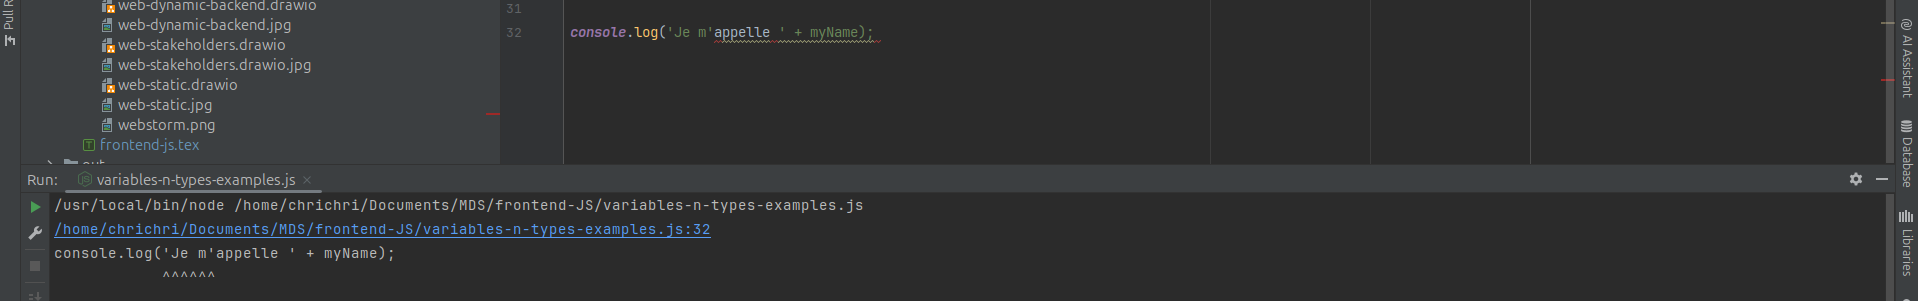
\includegraphics[width=12cm]{image/wrong-quote}
        \pause
        \bigbreak
        \flushleft
        Il faut des doubles quotes, mais on aurait pu s'en apercevoir avant, lors du développement, avec les avertissements en rouge dans l'IDE~.
    \end{frame}

    \begin{frame}[fragile]{Déclarations et types}{Les booléens}
        \begin{footnotesize}
            \begin{itemize}
                \item En JavaScript, un booléen est un type de donnée qui ne peut avoir que deux
                valeurs~: \lstinline{true} (vrai) ou \lstinline{false} (faux).
                \item Les booléens sont souvent utilisés dans les structures de contrôle comme les
                conditions (\lstinline{if}, \lstinline{else}) et les boucles
                (\lstinline{while}, \lstinline{for}).
                \item Les expressions booléennes sont des expressions qui évaluent à
                \lstinline{true} ou \lstinline{false}.
                \item Les opérateurs de comparaison (comme \lstinline{==}, \lstinline{===},
                \lstinline{!=}, \lstinline{!==}, \lstinline{>}, \lstinline{<},
                \lstinline{>=}, \lstinline{<=}) et les opérateurs logiques (comme
                \lstinline{&&}, \lstinline{||}, \lstinline{!}) sont utilisés pour créer des
                expressions booléennes.
            \end{itemize}
        \end{footnotesize}
        \begin{lstlisting}[language=Bash,title={\tiny{Node.js}},basicstyle=\tiny\ttfamily]
> var isAdult = true;
undefined
> var isMinor = false;
undefined
>
> if (isAdult) {
    ... console.log("Vous êtes un adulte.");
    ... } else {
    ... console.log("Vous êtes un mineur.");
    ... }
Vous êtes un adulte.
        \end{lstlisting}
    \end{frame}

    \begin{frame}[fragile]{Déclarations et types}{Les booléens}
        Tester le contraire d'un booléan avec \lstinline{!}~:
        \begin{lstlisting}[language=Bash,title={\tiny{Node.js}}]
> var isAdult = true;
undefined
> var isMinor = false;
undefined
>
> if (!isMinor) {
    ... console.log("Vous êtes un adulte.");
    ... } else {
    ... console.log("Vous êtes un mineur.");
    ... }
Vous êtes un adulte.
        \end{lstlisting}
    \end{frame}

    \begin{frame}[fragile]{Déclarations et types}{Les booléens}
        Le booléen \lstinline{false} est un entier de valeur 0, tout le reste est \lstinline{true}.
        \bigbreak
        On peut le vérifier en explicitant le type avec \lstinline{Boolean}~:
        \begin{lstlisting}[language=Bash,title={\tiny{Node.js}}]
> var isAdult = Boolean(0);
undefined
> isAdult
false
> var isAdult = Boolean(1)
undefined
> isAdult
true
> var isAdult = Boolean(25)
undefined
> isAdult
true
        \end{lstlisting}
    \end{frame}

    \begin{frame}[fragile]{Déclarations et types}{Les valeurs vides}
        \begin{footnotesize}
            Il existe deux valeurs spéciales, écrites \lstinline{null} et \lstinline{undefined}, qui sont utilisées pour indiquer l'absence de valeur significative.
            Elles sont elles-mêmes des valeurs, mais elles ne contiennent aucune information.

            De nombreuses opérations dans le langage qui ne produisent pas de valeur
            significative renvoient \lstinline{undefined} simplement parce qu'elles doivent
            renvoyer une valeur.

            La différence de signification entre \lstinline{undefined} et \lstinline{null}
            est un accident de la conception de JavaScript, et cela n'a pas d'importance la
            plupart du temps.
            Dans les cas où vous devez réellement vous préoccuper de ces
            valeurs, je recommande de les traiter comme étant principalement
            interchangeables.
        \end{footnotesize}
        \begin{lstlisting}[language=Bash,title={\tiny{Node.js}},basicstyle=\tiny\ttfamily]
> var parkingLot;
undefined
> parkingLot
undefined
> var parkingLot2 = null;
undefined
> parkingLot == parkingLot2
true
        \end{lstlisting}
    \end{frame}

    \begin{frame}[fragile]{Déclarations et types}{Déclaration de manière explicite}
        Déclarer le type de manière explicite pour éviter des ambiguïtés~:
        \begin{lstlisting}[language=Bash,title={\tiny{Node.js}}]
> var t = String(9)
undefined
> t
'9'
> var t = Number("9")
undefined
> t
9
        \end{lstlisting}
        \begin{dangercolorbox}
            De manière générale, en programmation, il est considéré plus \textit{safe} d'être explicite.

            On dit souvent \textit{Explicit is better than implicit}.
        \end{dangercolorbox}
    \end{frame}

    \begin{frame}[fragile]{Déclarations et types}{Portée d'une variable\footnote{\label{label}\lstinline{let}, Mozilla, \url{https://developer.mozilla.org/fr/docs/Web/JavaScript/Reference/Statements/let}}}
        \begin{small}
            On peut déclarer une variable de deux manières~:
            \begin{itemize}
                \item Avec le mot clé \lstinline{var}, la variable est \textit{globale} ou
                \textit{fonctionnelle}.
                \item Avec le mot clé \lstinline{let}, la variable est défini pour un \textit{de
                bloc} délimité par les \lstinline[language=Javascript]!{ }! d'une boucle,
                condition, fonction, \textit{etc}.
            \end{itemize}
        \end{small}
        \begin{lstlisting}[language=Bash,title={\tiny{Node.js}},basicstyle=\tiny\ttfamily]
undefined
> function x() {
    ... y = 1; // Lève une exception ReferenceError en mode strict
    ... var z = 2;
    ... }
undefined
> x();
undefined
> console.log(y); // Affiche "1" dans la console
1
undefined
> console.log(z); // Lève une exception ReferenceError car la portée est fonctionnelle:
Uncaught ReferenceError: z is not defined
        \end{lstlisting}
    \end{frame}

    \begin{frame}[fragile]{Déclarations et types}{Portée d'une variable\cref{label}}
        \begin{lstlisting}[language=Bash,title={\tiny{Node.js}},basicstyle=\tiny\ttfamily]
> let x = 1;
undefined
> if (x === 1) {
    ... let x = 2;
    ...
    ... console.log(x);
    ... // Expected output: 2
    ... }
2
undefined
> console.log(x);
1
        \end{lstlisting}
        La modification de
        \lstinline{x} dans la condition n'a pas modifié le \lstinline{x} déclaré avant.
        \begin{dangercolorbox}
            Éviter d'utiliser \lstinline{var} pour déclarer des variables, préférer \lstinline{let} pour éviter les erreurs de portée.

            L'état d'une variable globale peut être difficile à analyser sur la totalité
            d'un programme.
        \end{dangercolorbox}
    \end{frame}

    \begin{frame}[fragile]{Déclarations et types}{Les constantes\footnote{\lstinline{const}, Mozilla, \url{https://developer.mozilla.org/fr/docs/Web/JavaScript/Reference/Statements/const}}}
        \begin{footnotesize}
            On peut déclarer une constante avec le mot clé \lstinline{const}.
            Par la suite, cette constante n'est accessible qu'en lecture.
            Une nouvelle valeur ne peut lui être affectée, une variable du même nom ne peut être à nouveau déclarée.
            \begin{lstlisting}[language=Bash,title={\tiny{Node.js}},basicstyle=\tiny\ttfamily]
> const number = 42;
undefined
> try {
        ... number = 99;
        ... } catch (err) {
        ... console.log(err);
        ... }
TypeError: Assignment to constant variable.
at REPL9:2:10
...
undefined
> console.log(number); // Pas de réassignation mais première valeur
42
            \end{lstlisting}
            \begin{dangercolorbox}
                Penser au fonctionnel de l'application et utiliser des \lstinline{const} dès que possible par sécurité, pour éviter des modifications non souhaitables.
            \end{dangercolorbox}
        \end{footnotesize}
    \end{frame}

    \begin{frame}[fragile]{Déclarations et types}{Les étranges conversions automatiques de type}
        \begin{footnotesize}
            JavaScript est très flexible en ce qui concerne les types de données.
            Il convertit silencieusement de nombreux types de valeurs en d'autres types, pour que les choses fonctionnent comme prévu, c'est la \textit{type coercion}.
            Cela peut être pratique, mais parfois peu logique et donc peut aussi être source d'erreurs.
        \end{footnotesize}
        \begin{lstlisting}[language=Bash,title={\tiny{Node.js}},basicstyle=\tiny\ttfamily]
> console.log(8 * null)
0
undefined
> console.log("5" - 1)
4
undefined
> console.log("5" + 1)
51
undefined
> console.log("five" * 2)
NaN
undefined
> console.log(false == 0)
true
undefined
> console.log(null == undefined);
true
undefined
> console.log(null == 0);
false
        \end{lstlisting}
    \end{frame}

    \subsection{Les opérateurs}\label{subsec:operators}
    \begin{frame}{Les opérateurs\footnote{\label{operators}Expressions et opérateurs, \url{https://developer.mozilla.org/fr/docs/Web/JavaScript/Guide/Expressions_and_operators}}}
        \begin{tiny}
            \begin{table}[h!]
                \centering
                \begin{tabular}{|c|c|p{8cm}|}
                    \hline
                    \textbf{Operator}                     & \textbf{Type} & \textbf{Description}             \\
                    \hline
                    \lstinline[language=Javascript]!+!    & Binary        & Addition or string concatenation \\
                    \hline
                    \lstinline[language=Javascript]!-!    & Binary        & Subtraction                      \\
                    \hline
                    \lstinline[language=Javascript]!*!    & Binary        & Multiplication                   \\
                    \hline
                    \lstinline[language=Javascript]!/!    & Binary        & Division                         \\
                    \hline
                    \lstinline[language=Javascript]!\%!   & Binary        & Modulus (remainder)              \\
                    \hline
                    \lstinline[language=Javascript]!++!   & Unary         & Increment                        \\
                    \hline
                    \lstinline[language=Javascript]!--!   & Unary         & Decrement                        \\
                    \hline
                    \lstinline[language=Javascript]|!|    & Unary         & Logical NOT                      \\
                    \hline
                    \lstinline[language=Javascript]!==!   & Binary        & Equality (abstract comparison)   \\
                    \hline
                    \lstinline[language=Javascript]!===!  & Binary        & Strict equality                  \\
                    \hline
                    \lstinline[language=Javascript]|!=|   & Binary        & Inequality (abstract comparison) \\
                    \hline
                    \lstinline[language=Javascript]|!==|  & Binary        & Strict inequality                \\
                    \hline
                    \lstinline[language=Javascript]!>!    & Binary        & Greater than                     \\
                    \hline
                    \lstinline[language=Javascript]!<!    & Binary        & Less than                        \\
                    \hline
                    \lstinline[language=Javascript]!>=!   & Binary        & Greater than or equal to         \\
                    \hline
                    \lstinline[language=Javascript]!<=!   & Binary        & Less than or equal to            \\
                    \hline
                    \lstinline[language=Javascript]!\&\&! & Binary        & Logical AND                      \\
                    \hline
                    \lstinline[language=Javascript]!||!   & Binary        & Logical OR                       \\
                    \hline
                    \lstinline[language=Javascript]!?:!   & Ternary       & Conditional (ternary) operator   \\
                    \hline
                    \lstinline[language=Javascript]!=!    & Binary        & Assignment                       \\
                    \hline
                    \lstinline[language=Javascript]!+=!   & Binary        & Addition assignment              \\
                    \hline
                    \lstinline[language=Javascript]!-=!   & Binary        & Subtraction assignment           \\
                    \hline
                    \lstinline[language=Javascript]!*=!   & Binary        & Multiplication assignment        \\
                    \hline
                    \lstinline[language=Javascript]!/=!   & Binary        & Division assignment              \\
                    \hline
                    \lstinline[language=Javascript]!\%=!  & Binary        & Modulus assignment               \\
                    \hline
                \end{tabular}
            \end{table}
        \end{tiny}
    \end{frame}

    \begin{frame}[fragile]{Les opérateurs}{Les opérateurs de comparaison\cref{operators}}
        \begin{tiny}
            \begin{table}[h!]
                \centering
                \begin{tabular}{|c|p{4cm}|c|}
                    \hline
                    \textbf{Opérateur}                                       & \textbf{Description}                                                                                                                                                               & \textbf{Exemple qui renvoie \lstinline[language=Javascript]!true!} \\
                    \hline
                    Égalité (\lstinline[language=Javascript]!==!)            & Renvoie \lstinline[language=Javascript]!true! si les opérandes sont égaux (après conversion implicite).                                                                            & \lstinline[language=Javascript]!3 == '3'!                          \\
                    \hline
                    Inégalité (\lstinline[language=Javascript]|!=|)          & Renvoie \lstinline[language=Javascript]!true! si les opérandes sont différents (après conversion implicite).                                                                       & \lstinline[language=Javascript]|var2 != "3"|                       \\
                    \hline
                    Égalité stricte (\lstinline[language=Javascript]!===!)   & Renvoie \lstinline[language=Javascript]!true! si les opérandes sont égaux et du même type. Voir également \lstinline[language=Javascript]!Object.is()! et l'égalité en JavaScript. & \lstinline[language=Javascript]!3 === var1!                        \\
                    \hline
                    Inégalité stricte (\lstinline[language=Javascript]|!==|) & Renvoie \lstinline[language=Javascript]!true! si les opérandes sont du même type et différents ou s'ils ne sont pas du même type.                                                  & \lstinline[language=Javascript]|3 !== '3'|                         \\
                    \hline
                    Supériorité stricte (\lstinline[language=Javascript]!>!) & Renvoie \lstinline[language=Javascript]!true! si l'opérande gauche est strictement supérieur à l'opérande droit.                                                                   & \lstinline[language=Javascript]!'12' > 2!                          \\
                    \hline
                    Supériorité (\lstinline[language=Javascript]!>=!)        & Renvoie \lstinline[language=Javascript]!true! si l'opérande gauche est supérieur ou égal à l'opérande droit.                                                                       & \lstinline[language=Javascript]!var1 >= 3!                         \\
                    \hline
                    Infériorité stricte (\lstinline[language=Javascript]!<!) & Renvoie \lstinline[language=Javascript]!true! si l'opérande gauche est strictement inférieur à l'opérande droit.                                                                   & \lstinline[language=Javascript]!"2" < 12!                          \\
                    \hline
                    Infériorité (\lstinline[language=Javascript]!<=!)        & Renvoie \lstinline[language=Javascript]!true! si l'opérande gauche est inférieur ou égal à l'opérande droit.                                                                       & \lstinline[language=Javascript]!var2 <= 5!                         \\
                    \hline
                \end{tabular}
            \end{table}
        \end{tiny}
    \end{frame}

    \begin{frame}{Les opérateurs}{Les opérateurs de comparaison\cref{operators}}
        Exercice \execcounterdispinc{}~:
        \begin{itemize}
            \item Quand on compare des chaines de caractères, quel est l'ordre des caractères
            alphanumériques (lettres et chiffres)~?
            \item Comparer \lstinline{null} avec \lstinline{0} et aussi \lstinline{Infinity}.
            Est-ce logique~?
            \item Comparer \lstinline{null} avec \lstinline{undefined}.
            Est-ce logique~?
        \end{itemize}
        \bigbreak
        \centering
        
\includegraphics[width=3cm]{image/intelligence}
    \end{frame}

    \begin{frame}{Les opérateurs}{Les opérateurs arithmétiques\cref{operators}}
        \begin{tiny}
            \begin{table}[h!]
                \centering
                \begin{tabular}{|c|p{4cm}|p{4cm}|}
                    \hline
                    \textbf{Opérateur}                                  & \textbf{Description}                                                                                                                                                                                                                                                                   & \textbf{Exemple}                                                                                                                                                                                                                                                                                              \\
                    \hline
                    Addition (\lstinline[language=Javascript]!+!)       & Un opérateur binaire qui ajoute deux opérandes. Si les deux opérandes sont des nombres, ils sont additionnés. Si les deux opérandes sont des chaînes de caractères, elles sont concaténées. Si un opérande est une chaîne de caractères, l'autre est converti en chaîne de caractères. & \lstinline[language=Javascript]!3 + 4! renvoie \lstinline[language=Javascript]!7!. \newline \lstinline[language=Javascript]!"Hello" + " " + "World"! renvoie \lstinline[language=Javascript]!"Hello World"!. \newline \lstinline[language=Javascript]!"3" + 4! renvoie \lstinline[language=Javascript]!"34"!. \\
                    \hline
                    Soustraction (\lstinline[language=Javascript]!-!)   & Un opérateur binaire qui soustrait le deuxième opérande du premier.                                                                                                                                                                                                                    & \lstinline[language=Javascript]!3 - 4! renvoie \lstinline[language=Javascript]!-1!.                                                                                                                                                                                                                           \\
                    \hline
                    Multiplication (\lstinline[language=Javascript]!*!) & Un opérateur binaire qui multiplie les deux opérandes.                                                                                                                                                                                                                                 & \lstinline[language=Javascript]!3 * 4! renvoie \lstinline[language=Javascript]!12!.                                                                                                                                                                                                                           \\
                    \hline
                    Division (\lstinline[language=Javascript]!/!)       & Un opérateur binaire qui divise le premier opérande par le deuxième.                                                                                                                                                                                                                   & \lstinline[language=Javascript]!12 / 4! renvoie \lstinline[language=Javascript]!3!.                                                                                                                                                                                                                           \\
                    \hline
                    Reste (\lstinline[language=Javascript]!\%!)         & Un opérateur binaire qui renvoie le reste entier de la division des deux opérandes.                                                                                                                                                                                                    & \lstinline[language=Javascript]!12 \% 5! renvoie \lstinline[language=Javascript]!2!.                                                                                                                                                                                                                          \\
                    \hline
                \end{tabular}
            \end{table}
        \end{tiny}
    \end{frame}

    \begin{frame}{Les opérateurs}{Les opérateurs arithmétiques\cref{operators}}
        \begin{tiny}
            \begin{table}[h!]
                \centering
                \begin{tabular}{|c|p{4cm}|p{4cm}|}
                    \hline
                    \textbf{Opérateur}                                               & \textbf{Description}                                                                                                                                                                                                                                                                                                                & \textbf{Exemple}                                                                                                                                                                                                                                                                                                                                                                                                                                                  \\
                    \hline
                    Incrément (\lstinline[language=Javascript]!++!)                  & Un opérateur unaire qui ajoute un à son opérande. S'il est utilisé en opérateur préfixe (\lstinline[language=Javascript]!++x!), il renvoie la valeur de son opérande après y avoir ajouté un. S'il est utilisé en opérateur suffixé (\lstinline[language=Javascript]!x++!), il renvoie la valeur de l'opérande avant l'ajout de un. & Si \lstinline[language=Javascript]!x! vaut 3, alors \lstinline[language=Javascript]!++x! définit \lstinline[language=Javascript]!x! avec \lstinline[language=Javascript]!4! et renvoie \lstinline[language=Javascript]!4!, tandis que \lstinline[language=Javascript]!x++! renvoie \lstinline[language=Javascript]!3! puis, uniquement après, définit \lstinline[language=Javascript]!x! avec \lstinline[language=Javascript]!4!.                                 \\
                    \hline
                    Décrément (\lstinline[language=Javascript]!--!)                  & Un opérateur unaire qui soustrait un à son opérande. La valeur de retour est analogue à celle de l'opérateur d'incrément.                                                                                                                                                                                                           & Si \lstinline[language=Javascript]!x! vaut \lstinline[language=Javascript]!3!, alors \lstinline[language=Javascript]!--x! définit \lstinline[language=Javascript]!x! avec \lstinline[language=Javascript]!2! et renvoie \lstinline[language=Javascript]!2!, tandis que \lstinline[language=Javascript]!x--! renvoie \lstinline[language=Javascript]!3! puis, uniquement après, définit \lstinline[language=Javascript]!x! avec \lstinline[language=Javascript]!2! \\
                    \hline
                    Négation unaire (\lstinline[language=Javascript]!-!)             & Un opérateur unaire qui renvoie l'opposé de l'opérande.                                                                                                                                                                                                                                                                             & Si \lstinline[language=Javascript]!x! vaut 3, \lstinline[language=Javascript]!-x! renvoie \lstinline[language=Javascript]!-3!.                                                                                                                                                                                                                                                                                                                                    \\
                    \hline
                    Plus unaire (\lstinline[language=Javascript]!+!)                 & Un opérateur unaire qui tente la conversion de l'opérande en nombre si ce n'est pas déjà une valeur numérique.                                                                                                                                                                                                                      & \lstinline[language=Javascript]!+"3"! renvoie \lstinline[language=Javascript]!3!. \newline \lstinline[language=Javascript]!+true! renvoie \lstinline[language=Javascript]!1!.                                                                                                                                                                                                                                                                                     \\
                    \hline
                    Opérateur d'exponentiation (\lstinline[language=Javascript]!**!) & Élève une base donnée par l'opérande gauche à la puissance donnée par l'opérande droite.                                                                                                                                                                                                                                            & \lstinline[language=Javascript]!2 ** 3! renvoie \lstinline[language=Javascript]!8!. \newline \lstinline[language=Javascript]!10 ** -1! renvoie \lstinline[language=Javascript]!0.1!.                                                                                                                                                                                                                                                                              \\
                    \hline
                \end{tabular}
            \end{table}
        \end{tiny}
    \end{frame}

    \begin{frame}{Les opérateurs}{Les opérateurs arithmétiques\cref{operators}}
        Exercice \execcounterdispinc{}~:
        \begin{itemize}
            \item Quelle est la différence entre \lstinline{++x} et \lstinline{x++}~?
            \item Quelle est la différence entre \lstinline{Infinity} et \lstinline{Infinity}~?
            \item Quelle est la différence entre \lstinline{null} et \lstinline{undefined}~?
            Est-ce logique par rapport à ce que nous avons vu précédemment avec les
            opérateurs de comparaison~?
            \item Additionner deux chaines de caractères.
            \item Soustraire deux chaines de caractères.
            Étonnant non~?
            \item Utiliser
            \lstinline{\%} pour vérifier si un nombre est pair ou impair et \lstinline{==}.
        \end{itemize}
        \bigbreak
        \centering
        
\includegraphics[width=3cm]{image/intelligence}
    \end{frame}

    \begin{frame}{Les opérateurs}{Opérateurs logiques\cref{operators}}
        \begin{scriptsize}
            Les plus utilisés\ldots
            \begin{table}[h!]
                \centering
                \begin{tabular}{|c|c|p{7cm}|}
                    \hline
                    \textbf{Opérateur}                               & \textbf{Utilisation}                              & \textbf{Description}                                                                                                                                                                                                                                                                                                                                                                                                                                                                         \\
                    \hline
                    ET logique \lstinline[language=Javascript]!\&\&! & \lstinline[language=Javascript]!expr1 \&\& expr2! & Renvoie \lstinline[language=Javascript]!expr1! si elle peut être convertie en \lstinline[language=Javascript]!false! et renvoie \lstinline[language=Javascript]!expr2! sinon. Lorsqu'il est utilisé avec des valeurs booléennes, \lstinline[language=Javascript]!\&\&! renvoie \lstinline[language=Javascript]!true! si les deux opérandes valent \lstinline[language=Javascript]!true! et \lstinline[language=Javascript]!false! sinon.                                                     \\
                    \hline
                    OU logique \lstinline[language=Javascript]!||!   & \lstinline[language=Javascript]!expr1 || expr2!   & Renvoie \lstinline[language=Javascript]!expr1! si elle peut être convertie en \lstinline[language=Javascript]!true! et renvoie \lstinline[language=Javascript]!expr2! sinon. Lorsqu'il est utilisé avec des valeurs booléennes, \lstinline[language=Javascript]!||! renvoie \lstinline[language=Javascript]!true! si l'un des deux opérandes vaut \lstinline[language=Javascript]!true! et \lstinline[language=Javascript]!false! si les deux valent \lstinline[language=Javascript]!false!. \\
                    \hline
                    NON logique \lstinline[language=Javascript]|!|   & \lstinline[language=Javascript]|!expr|            & Renvoie \lstinline[language=Javascript]!false! si son unique opérande peut être converti en \lstinline[language=Javascript]!true!, renvoie \lstinline[language=Javascript]!true! sinon.                                                                                                                                                                                                                                                                                                      \\
                    \hline
                \end{tabular}
            \end{table}
            \begin{dangercolorbox}
                Ne pas confondre \lstinline{||} et \lstinline{|}, \lstinline{\&\&} et \lstinline{\&}.
                Les logiques, comme ici, évaluent le membre différent de \lstinline{0} si l'expression est \lstinline{true}.
            \end{dangercolorbox}
        \end{scriptsize}
    \end{frame}

    \begin{frame}[fragile]{Les opérateurs}{Opérateur conditionnel A.K.A. ternaire}
        \begin{small}
            L'opérateur conditionnel est le seul opérateur JavaScript à prendre trois opérandes. Il permet d'affecter une valeur ou en affecter une autre selon une condition donnée. Sa syntaxe est la suivante~:
            \begin{lstlisting}[language=JavaScript,title={\tiny{Script JavaScript}},basicstyle=\tiny\ttfamily]
condition ? val1 : val2;
            \end{lstlisting}
            Si la condition est vraie, l'expression sera résolue avec la valeur de \lstinline{val1}.
            Sinon, elle sera résolue avec la valeur de \lstinline{val2}.
            L'opérateur conditionnel peut être utilisé à tout endroit où un opérateur
            standard peut être utilisé. \bigbreak Par exemple~:
            \begin{lstlisting}[language=Bash,title={\tiny{Node.js}},basicstyle=\tiny\ttfamily]
> let age = 19;
undefined
> const statut = age >= 18 ? "adulte" : "mineur";
undefined
> statut
'adulte'
            \end{lstlisting}
            Cette instruction affecte la valeur
            \lstinline{"adulte"} à la variable \lstinline{statut} si \lstinline{age} est supérieur ou égal à 18.
            Sinon, c'est la valeur \lstinline{"mineur"} qui est affectée à \lstinline{statut}.
        \end{small}
    \end{frame}

    \begin{frame}{Les opérateurs}{Opérateur conditionnel A.K.A. ternaire}
        Exercice \execcounterdispinc{}~:
        \begin{itemize}
            \item Stocker un booléen dans \lstinline{major} si la variable \lstinline{age} est
            supérieur à 18.
            \item Stocker la chaîne de caractère
            \lstinline{pair} dans la variable \lstinline{pairOrImpair} si
            \lstinline{x} est pair, sinon stocker la chaîne de caractère \lstinline{impair}.
            \item Stocker un booléen dans \lstinline{pairBool} si \lstinline{x} est pair.
        \end{itemize}
        \bigbreak
        \centering
        
\includegraphics[width=3cm]{image/intelligence}
    \end{frame}

    \begin{frame}{Les opérateurs}{Opérateurs binaires\cref{operators}}
        \begin{scriptsize}
            Pas les plus utilisés\ldots
            \begin{table}[h!]
                \centering
                \begin{tabular}{|p{3cm}|c|p{6cm}|}
                    \hline
                    \textbf{Opérateur}                                                      & \textbf{Utilisation}                     & \textbf{Description}                                                                                                                                                                                                           \\
                    \hline
                    ET binaire                                                              & \lstinline[language=Javascript]!a \& b!  & Renvoie \lstinline[language=Javascript]!1! à chaque position pour laquelle les bits des deux opérandes valent \lstinline[language=Javascript]!1!.                                                                              \\
                    \hline
                    OU binaire                                                              & \lstinline[language=Javascript]!a | b!   & Renvoie \lstinline[language=Javascript]!0! à chaque position pour laquelle les bits des deux opérandes valent \lstinline[language=Javascript]!0!.                                                                              \\
                    \hline
                    OU exclusif binaire                                                     & \lstinline[language=Javascript]!a \^ b!  & Renvoie \lstinline[language=Javascript]!0! à chaque position pour laquelle les bits sont les mêmes. Renvoie \lstinline[language=Javascript]!1! à chaque position où les bits sont différents.                                  \\
                    \hline
                    NON binaire                                                             & \lstinline[language=Javascript]!\~a!     & Inverse les bits de l'opérande.                                                                                                                                                                                                \\
                    \hline
                    Décalage à gauche                                                       & \lstinline[language=Javascript]! a << b! & Décale la représentation binaire de \lstinline[language=Javascript]!a! de \lstinline[language=Javascript]!b! bits vers la gauche, en ajoutant des \lstinline[language=Javascript]!0! à droite.                                 \\
                    \hline
                    Décalage à droite avec propagation du signe                             & \lstinline[language=Javascript]!a >> b!  & Décale la représentation binaire de \lstinline[language=Javascript]!a! de \lstinline[language=Javascript]!b! bits vers la droite, en enlevant les bits en trop.                                                                \\
                    \hline
                    Décalage à droite avec remplissage à \lstinline[language=Javascript]!0! & \lstinline[language=Javascript]!a >>> b! & Décale la représentation binaire de \lstinline[language=Javascript]!a! de \lstinline[language=Javascript]!b! bits vers la droite, en enlevant les bits en trop et en ajoutant des \lstinline[language=Javascript]!0! à gauche. \\
                    \hline
                \end{tabular}
            \end{table}
            \begin{dangercolorbox}
                Ne pas confondre \lstinline{||} et \lstinline{|}, \lstinline{\&\&} et \lstinline{\&}.
                Les binaires comme ici, renvoient toujours \lstinline{0} ou \lstinline{1}, les autres, les logiques évaluent le membre différent de \lstinline{0}.
            \end{dangercolorbox}
        \end{scriptsize}
    \end{frame}

    \begin{frame}{Les opérateurs}{Opérateurs binaires\cref{operators}}
        Certaines anciennes machines et programmes utilisaient les opérateurs binaires pour accélérer l'arithmétique.
        Par exemple le décalage à gauche \lstinline[language=Javascript]! a << b! est équivalent à \lstinline{a * 2^b}.
        Le décalage à droite \lstinline[language=Javascript]! a >> b! est équivalent à \lstinline{a / 2^b}.
        \bigbreak
        Exercice \execcounterdispinc{}~:
        \begin{itemize}
            \item Stocker dans la variable
            \lstinline{multBySixtyFour} l'entier égal à \lstinline{8 * 64} en utilisant un
            opérateur binaire.
            \item Stocker dans la variable
            \lstinline{divBySixtyFour} l'entier égal à \lstinline{512 / 32} en utilisant un
            opérateur binaire.
            \item Vérifier que \lstinline{x \&1} permet de vérifier que \lstinline{x} est impair.
            \item À partir de l'expression \lstinline{x \&1} quel opérateur peut-on utiliser pour vérifier que est pair~?
            \item Stocker un booléen dans \lstinline{pairBool} si \lstinline{x} est pair à l'aide
            de l'opérateur \lstinline{\&} et de la déclaration de type \lstinline{Boolean}.
        \end{itemize}
    \end{frame}

    \subsection{Les fonctions}\label{subsec:functions}
    \begin{frame}[fragile]{Les fonctions}{Déclarations\footnote{\label{mozilla-function}Définir des fonctions, Mozilla, \url{https://developer.mozilla.org/fr/docs/Web/JavaScript/Guide/Functions}}}
        \begin{small}
            Une définition de fonction (aussi appelée déclaration de fonction ou instruction de fonction) est construite avec le mot-clé \href{https://developer.mozilla.org/fr/docs/Web/JavaScript/Reference/Statements/function}{function}, suivi par~:
            \begin{itemize}
                \item L'éventuel nom de la fonction, sinon c'est une fonction anonyme.
                \item Une \textbf{éventuelle} liste d'arguments à passer à la fonction, entre
                parenthèses et séparés par des virgules.
                \item Les instructions JavaScript définissant la fonction, entre accolades,
                \lstinline[language=Javascript]!{ }!.
                \item L'\textbf{éventuel} instruction
                \lstinline{return} si la fonction doit renvoyer une valeur, un objet, \textit{etc}.
            \end{itemize}
        \end{small}
        \bigbreak
        Le code suivant, par exemple, définit une fonction intitulée square~:
        \begin{lstlisting}[language=JavaScript,title={\tiny{Script JavaScript}}]
function square(number){
    return number * number;
}
        \end{lstlisting}
    \end{frame}

    \begin{frame}[fragile]{Les fonctions}{Déclarations\cref{mozilla-function}}
        La fonction square prend un seul argument, appelé number.
        La fonction est composée d'une seule instruction qui renvoie l'argument de la fonction (number) multiplié par lui-même.
        L'instruction \href{https://developer.mozilla.org/fr/docs/Web/JavaScript/Reference/Statements/return}{return} spécifie la valeur qui est renvoyée par la fonction.~:
        \begin{lstlisting}[language=JavaScript,title={\tiny{Script JavaScript}}]
return number * number;
        \end{lstlisting}
        \begin{dangercolorbox}
            Les paramètres primitifs (comme les nombres) sont passés à la fonction par valeur.
            La valeur est passée à la fonction mais si cette dernière change la valeur du paramètre, cela n'aura pas d'impact au niveau global ou au niveau de ce qui a appelé la fonction.
        \end{dangercolorbox}
        Qu'est-ce que ça veut dire~?
    \end{frame}

    \begin{frame}[fragile]{Les fonctions}{Déclarations\cref{mozilla-function}}
        Des valeurs par défaut peuvent être définies pour les arguments de la fonction.
        Ils sont toujours placés après les arguments qui n'en n'ont pas.
        \begin{lstlisting}[language=JavaScript,title={\tiny{Script JavaScript}}]
function multiply(a, b=1) {
    return a*b;
}
        \end{lstlisting}
        Ici, il n'est pas obligatoire de définir \lstinline{1} car il a une valeur par défaut~:
        \begin{lstlisting}[language=Bash,title={\tiny{Node.js}}]
> function multiply(a, b = 1) {
...     return a*b;
... }
undefined
> multiply(2) // a est 2, b est 1
2
> multiply(2, 2) // a est 2, b est 2
4
        \end{lstlisting}
    \end{frame}

    \begin{frame}{Les fonctions}{Les caractéristiques et bonnes pratiques}
        \begin{itemize}
            \item Elles sont courtes, sont atomiques et font une seule chose. Mieux vaut les
            imbriquer que d'avoir une grosse fonction complexe.
            \item Elles sont nommées de manière explicite, avec un verbe décrivant leur action.
            \item Leurs commentaires sont simples car elles sont simples.
            \item Peuvent appeler d'autres fonctions ou s'appeler elle-même (fonction récursive).
            \item On les sépare en 2 familles~:
            \begin{itemize}
                \item Les fonctions \textit{pures}, qui appliquent une transformation sur des données
                passées en argument et renvoient un résultat.
                Sans aucune action sur le environnement.
                \item Les fonctions \textit{avec effet de bord}, qui modifient l'environnement.
                Appel d'API, log dans la console, \textit{etc}.
            \end{itemize}
        \end{itemize}
    \end{frame}

    \begin{frame}[fragile]{Les fonctions}{Appeler une fonction\cref{mozilla-function}}
        Une fois que la fonction est définie, elle peut être appelée par son nom suivi de parenthèses et des arguments à passer à la fonction entre ces parenthèses.
        Par exemple, pour appeler la fonction carré définie précédemment.
        Par convention on termine l'appel par \lstinline{;}.
        Si la fonction a un \lstinline{return}, la valeur retournée peut être stockée dans une variables~:
        \begin{lstlisting}[language=Bash,title={\tiny{Node.js}}]
> function square(nombre) {
...     return nombre * nombre;
... }
undefined
> let twoSquared = square(2);
undefined
> twoSquared
4
> square(2);
4
        \end{lstlisting}
    \end{frame}

    \begin{frame}[fragile]{Les fonctions}{La portée de la fonction\cref{mozilla-function}}
        Il est possible d'imbriquer une fonction au sein d'une fonction.
        La fonction imbriquée (interne) est privée par rapport à la fonction (externe) qui la contient.
        Cela forme ce qu'on appelle une fermeture (\textit{closure} en anglais).
        \begin{lstlisting}[language=Bash,title={\tiny{Node.js}}]
> function ajouteCarres(a, b) {
... function carre(x) {
...         return x * x;
...     }
...     return carre(a) + carre(b);
... }
undefined
> let a = ajouteCarres(2, 3); // renvoie 13
undefined
> let b = ajouteCarres(3, 4); // renvoie 25
undefined
> let c = ajouteCarres(4, 5); // renvoie 41
        \end{lstlisting}
    \end{frame}

    \begin{frame}[fragile]{Les fonctions}{La portée de la fonction\cref{mozilla-function}}
        \begin{tiny}
            Une fermeture est une expression (généralement une fonction) possédant des variables libres ainsi qu'un environnement qui lie ces variables (autrement dit qui \textit{ferme} l'expression).
            \bigbreak
            Étant donné qu'une fonction imbriquée est une fermeture, cela signifie que la fonction imbriquée peut \textit{hériter} des arguments et des variables de la fonction qui la contient.
            En d'autres termes, la fonction interne contient la portée de la fonction externe.
            \bigbreak
            Pour résumer~:
            \begin{itemize}
                \item On ne peut accéder à la fonction interne seulement avec des instructions
                contenues dans la fonction externe.
                \item La fonction interne est une fermeture~: la fonction interne peut utiliser des
                arguments et des variables de la fonction externe alors que la fonction externe
                ne peut pas utiliser de variables et d'arguments de la fonction interne.
            \end{itemize}
        \end{tiny}
        \begin{lstlisting}[language=Bash,title={\tiny{Node.js}}]
function externe(x) {
    function interne(y) {
        return x + y;
    }
    return interne;
}
let fn_interne = externe(3);
let resultat = fn_interne(5); // renvoie 8

let resultat1 = externe(3)(5); // renvoie 8
undefined
> resultat
8
> resultat1
8
        \end{lstlisting}
    \end{frame}

    \begin{frame}{Les fonctions}{Exercice \execcounterdispinc{}}
        \begin{itemize}
            \item Développer une fonction récursive appelé \lstinline{factorial} qui prend en
            entrée un entier et calcul le factoriel.
            C'est donc une fonction pure.
            \item Appeler la fonction et trouver à quel nombre le factoriel est assimilé à
            \lstinline{Infinity}.
            \item Développer une seconde fonction avec effet de bord seulement, appelée
            \lstinline{displayFactorialResult}, qui affiche le résultat dans la console avec les fonctions \lstinline{console.log}
            et \lstinline{factorial}. Le message doit être~: \lstinline{"Le factoriel de 5
              est 120."}.
        \end{itemize}
        \bigbreak
        \centering
        
\includegraphics[width=3cm]{image/intelligence}
    \end{frame}

    \begin{frame}[fragile]{Les fonctions}{Les \textit{arrows functions}}
        La dernière norme ES6 a introduit les \textit{arrows functions} ou fonctions fléchées en bon français.
        Leur syntaxe est plus courte et parfois donc plus lisible.
        Elles peuvent aussi être anonymes.

        Cette syntaxe s'inspire de la programmation fonctionnelle et des fonctions
        \textit{lambda}.
        \begin{dangercolorbox}
            Les fonctions fléchées ne sont pas adaptées à tous les usages, il faut les réserver aux fonctions pures et simples.
        \end{dangercolorbox}
        La syntaxe est la suivante~:
        \begin{lstlisting}[language=JavaScript,title={\tiny{Script JavaScript}}]
function squareOldStyle(nombre) {
        return nombre * nombre;
    }
const squareArrowStyle = (nombre) => nombre * nombre;
        \end{lstlisting}
        \begin{dangercolorbox}
            Le \lstinline{return} est implicite~!
        \end{dangercolorbox}
    \end{frame}

    \begin{frame}{Les fonctions}{Exercice \execcounterdispinc{}}
        Que font ces packages JS en lignes~?
        \begin{itemize}
            \item \url{https://www.npmjs.com/package/is-odd}
            \item \url{https://www.npmjs.com/package/is-even}
            \item \url{https://www.npmjs.com/package/is-odd-ai}
            \item \url{https://www.npmjs.com/package/is-even-ai}
        \end{itemize}
        Est-ce utile?
        \bigbreak
        Est-ce dangereux~?
        \bigbreak
        \centering
        
\includegraphics[width=3cm]{image/intelligence}
    \end{frame}

    \begin{frame}{Les fonctions}{Exercice \execcounterdispinc{}}
        Développer les mêmes fonctions avec des fonctions fléchées en un minimum de caractères/ligne de code possible (Moins de code = moins de bugs \emoji{wink}).
        \bigbreak
        \begin{itemize}
            \item La fonction \lstinline{isOdd} qui renvoie \lstinline{true} si le nombre est
            impair.
            \item La fonction \lstinline{isEven} qui renvoie \lstinline{true} si le nombre est
            pair.
            \item Développer une fonction à partir de l'autre.
        \end{itemize}
        \bigbreak
        \centering
        
\includegraphics[width=3cm]{image/intelligence}
    \end{frame}

    \begin{frame}{Usage d'une fonction \textit{built-in}}{Exemple de la fonction \lstinline{Date}}
        Toutes les capacités, les fonctions, les objets, les méthodes, les propriétés de JavaScript sont documentés sur le site de Mozilla.
        \bigbreak
        \begin{dangercolorbox}
            En informatique on dit souvent \textit{RTFM} comme \textit{\textbf{R}ead \textbf{T}he \textbf{F}u***** \textbf{M}anual}, c'est le secret de la réussite.
        \end{dangercolorbox}
        \bigbreak
        On trouve la documentation de cette fonction à l'adresse \url{https://developer.mozilla.org/en-US/docs/Web/JavaScript/Reference/Global_Objects/Date}.
        \bigbreak
        Exercice \execcounterdispinc{}~:
        \begin{itemize}
            \item Lire la documentation.
            \item Utiliser la fonction \lstinline{Date} pour afficher la date et l'heure actuelle
            de manière lisible par un humain.
            \item Trouver une méthode qui permet de modifier la date d'un objet \lstinline{Date}.
        \end{itemize}
    \end{frame}

    \subsection{Les conditions}\label{subsec:conditions}

    \begin{frame}[fragile]{Structure if/else}
        \begin{itemize}
            \item Utilisée pour exécuter du code en fonction d'une condition.
            \item Syntaxe~:
        \end{itemize}
        \begin{lstlisting}[language=JavaScript,title={\tiny{Script JavaScript}}]
if (condition) {
    // code à exécuter si la condition est vraie
} else {
    // code à exécuter si la condition est fausse
}
        \end{lstlisting}
        On passe dans le
        \lstinline{if} si la condition peut être évaluée comme un booléen à \lstinline{true}.
        Sinon on passe dans le \lstinline{if}.
    \end{frame}

    \begin{frame}[fragile]{Exemple if/else}
        \begin{lstlisting}[language=JavaScript,title={\tiny{Script JavaScript}}]
let heure = 10;
if (heure < 12) {
    console.log("Bonjour");
} else {
    console.log("Bonsoir");
}
        \end{lstlisting}
    \end{frame}

    \begin{frame}[fragile]{Les \lstinline{if/else} imbriqués}
        Si il y a plusieurs conditions à vérifier, on peut imbriquer les \lstinline{if/else}.
        \bigbreak
        Mais cette structure est très peu lisible quand il y en a plus de 3.
        Exemple de \lstinline{if/else} imbriqués~:
        \begin{lstlisting}[language=JavaScript,title={\tiny{Script JavaScript}},basicstyle=\tiny\ttfamily]
let age = 25;
let citoyen = true;
let casierJudiciaire = false;

if (age >= 18) {
    if (citoyen) {
        if (!casierJudiciaire) {
            console.log("Vous êtes éligible pour voter.");
        } else {
            console.log("Vous n'êtes pas éligible pour voter en raison de votre casier judiciaire.");
        }
    } else {
        console.log("Vous n'êtes pas éligible pour voter, car vous n'êtes pas citoyen.");
    }
} else {
        console.log("Vous n'êtes pas éligible pour voter, car vous êtes mineur.");
}
        \end{lstlisting}
    \end{frame}

    \begin{frame}[fragile]{Les conditions multiples}
        Une condition peut être un ensemble de conditions reliées par un opérateur logique, ou/et.
        Sans aucune limite de nombre, si ce n'est celle de la lisibilité du code.
        \bigbreak
        Ajouter des parenthèses permet d'indiquer une priorité dans les conditions.
        La condition la plus prioritaire étant celle qui est la entourée du plus grand nombre de parenthèses.
        \begin{lstlisting}[language=JavaScript,title={\tiny{Script JavaScript}}]
let age = 25;
let citoyen = true;
let casierJudiciaire = false;

if (age >= 18 && citoyen && !casierJudiciaire) {
    console.log("Vous êtes éligible pour voter.");
} else {
    console.log("Vous n'êtes pas éligible pour voter.");
}
        \end{lstlisting}
    \end{frame}

    \begin{frame}[fragile]{Structure switch case}
        \begin{itemize}
            \item Utilisée pour exécuter différents blocs de code en fonction de différentes
            valeurs possibles d'une expression.
            Ou pour remplacer des \lstinline{if/else} imbriqués.
            \item Syntaxe~:
        \end{itemize}
        \begin{lstlisting}[language=JavaScript,title={\tiny{Script JavaScript}}]
switch (expression) {
    case valeur1:
    // code à exécuter si expression == valeur1
    break;
    case valeur2:
    // code à exécuter si expression == valeur2
    break;
    default:
    // code à exécuter si aucune des valeurs ne correspond ou absence de break
}
        \end{lstlisting}
        \lstinline{default} est optionnel et permet de définir un code à exécuter si aucune des valeurs ne correspond.
        \lstinline{break} permet de sortir du switch case et donc de ne pas passer dans \lstinline{default}.
    \end{frame}

    \begin{frame}[fragile]{Exemple switch case}
        \begin{lstlisting}[language=JavaScript,title={\tiny{Script JavaScript}}]
let jour = 3;
switch (jour) {
    case 1:
    console.log("Lundi");
    break;
    case 2:
    console.log("Mardi");
    break;
    case 3:
    console.log("Mercredi");
    break;
    default:
    console.log("Jour inconnu");
}
        \end{lstlisting}
    \end{frame}

    \begin{frame}{Les conditions dans une fonction}{Exercice \execcounterdispinc{}}
        Créer une fonction appelée \lstinline{typeDeTriangle} qui requiert~:
        \begin{itemize}
            \item 3 arguments de type \lstinline{Number} qui représentent les 3 côtés d'un triangle.
            \item La fonction doit renvoyer le type de triangle~:
            \begin{itemize}
                \item \lstinline{équilatéral} si les 3 côtés sont égaux.
                \item \lstinline{isocèle} si 2 côtés sont égaux.
                \item \lstinline{scalène} si les 3 côtés sont différents.
                \item \lstinline{non triangle} si les 3 côtés ne peuvent pas former un triangle.
                \item \lstinline{triangle rectangle} si le triangle est rectangle.
            \end{itemize}
        \end{itemize}
        \bigbreak
        \centering
        
\includegraphics[width=3cm]{image/intelligence}
    \end{frame}

    \begin{frame}{Les conditions dans une fonction}{Exercice \execcounterdispinc{}}
        \begin{footnotesize}
            Selon Wikipedia une année est bissextile si \footnote{Année bissextile, \url{https://fr.wikipedia.org/wiki/Ann\%C3\%A9e_bissextile}}~:
            \begin{textit}
                Les années sont bissextiles si elles sont multiples de 4, mais pas si elles sont multiples de 100, à l'exception des années multiples de 400 qui, elles, sont également bissextiles.
                Ainsi, les années 2020, 2024 et 2028 sont bissextiles, de même que 2000 ou 2400, mais pas 1900, 2100, 2200 et 2300.
            \end{textit}
            \bigbreak
            Créer une fonction appelée \lstinline{estBissextile} qui requiert~:
            \begin{itemize}
                \item 1 argument de type \lstinline{Number} qui représente une année.
                \item La fonction doit renvoyer \lstinline{true} si l'année est bissextile, \lstinline{false} sinon.
                \item Utiliser un \lstinline{if/else}.
            \end{itemize}
        \end{footnotesize}
        \bigbreak
        \centering
        
\includegraphics[width=3cm]{image/intelligence}
    \end{frame}


    \section{Collections, boucles et objets}\label{sec:collections-loops-objects}

    \begin{frame}{Les collections}
        \begin{footnotesize}
            En JavaScript, il existe des types natifs qui permettent de stocker plusieurs valeurs dans une seule variable.
            \bigbreak
            \begin{columns}
                \column{0.5\textwidth}
                Les collections sont entre autre~:
                \begin{itemize}
                    \item Les tableaux, ils stockent des valeurs de manière ordonnée.
                    \item Les objets, ils stockent des valeurs sous forme de clé/valeur.
                    \item Les ensembles, ils stockent des valeurs uniques.
                    \item Les \lstinline{Map}, ils stockent des valeurs sous forme de clé/valeur.
                \end{itemize}
                \column{0.5\textwidth}
                \centering
                
\includegraphics[width=5cm]{image/account-store}
            \end{columns}
            \flushleft
            Par exemple, dans un tableau on va stocker toutes les notes des étudiants pour faire des statistiques dessus (moyenne, médiane, \textit{etc}).

            Les objets sont plus comme des minis bases de données, on peut y stocker des informations sur un étudiant (nom, prénom, âge, notes, \textit{etc}).
        \end{footnotesize}
    \end{frame}

    \subsection{Les tableaux}\label{subsec:arrays}

    \begin{frame}[fragile]{Les collections}{Les tableaux}
        Le tableau ou aussi appelé objet de type \lstinline{Array} en JavaScript, porte de multiples méthodes pour lire ou modifier cette collection.
        \begin{itemize}
            \item Les arrays peuvent contenir différents types de donnée.
            \item Certains comme les \lstinline{Uint8Array}, \lstinline{Float32Array}, \textit{etc} sont des tableaux typés (pas le temps de les voir dans ce cours).
        \end{itemize}
        \begin{lstlisting}[language=JavaScript,title={\tiny{Script JavaScript}}]
let students = ["Alice", "Bob", "Charlie", "David"];
// Sinon en explicitant le type
let students = new Array("Alice", "Bob", "Charlie", "David");
        \end{lstlisting}
        \begin{dangercolorbox}
            À la différence des types primitifs, quand on spécifie ce dernier, il ajouter le mot-clé \lstinline{new}.

            Les tableaux sont des objets, ils sont donc passés par référence et non pas par copie comme les types primitifs.
        \end{dangercolorbox}
    \end{frame}

    \begin{frame}[fragile]{Les collections}{Accéder aux éléments d'un tableau\footnote{Accéder aux éléments d'un tableau, \url{https://developer.mozilla.org/fr/docs/Web/JavaScript/Reference/Global\_Objects/Array}}}
        Les tableaux sont indexés à partir de zéro.
        Le premier élément d'un tableau a pour indice 0 et la position du dernier élément est donnée par \href{https://developer.mozilla.org/fr/docs/Web/JavaScript/Reference/Global\_Objects/Array/length}{length} moins 1.
        Si on utilise un indice en dehors de cet intervalle, le résultat sera \href{https://developer.mozilla.org/fr/docs/Web/JavaScript/Reference/Global_Objects/undefined}{undefined} (sous réserve qu'aucune propriété n'ait été ajoutée au préalable avec cet indice).
        \begin{lstlisting}[language=JavaScript,title={\tiny{Script JavaScript}}]
let arr = ["le premier élément", "le deuxième élément", "le dernier élément"];
console.log(arr[0]); // affiche "le premier élément"
console.log(arr[1]); // affiche "le deuxième élément"
console.log(arr[arr.length - 1]); // affiche "le dernier élément"
console.log(arr[10]); // retourne undefined
        \end{lstlisting}
        La propriété \lstinline{length}, accessible avec la syntaxe \lstinline{arr.length} renvoie un entier égal à la taille du tableau.
    \end{frame}

    \begin{frame}{Les collections}{Les méthodes des tableaux}
        \begin{footnotesize}
            Les tableaux ont plusieurs propriétés qui permettent de les manipuler.
            Les essentielles~:
            \begin{itemize}
                \item \lstinline{push()}~: Ajoute un ou plusieurs éléments à la fin d'un tableau et renvoie la nouvelle longueur du tableau.
                \item \lstinline{splice()}~: Supprime un élément par son index
                \item \lstinline{concat()}~: Fusionne deux tableaux.
                \item \lstinline{forEach()}~: Exécute une fonction donnée une fois pour chaque élément du tableau.
                \item \lstinline{map()}~: Crée un nouveau tableau avec les résultats de l'appel d'une fonction (souvent une fonction fléchée) fournie sur chaque élément du tableau. \textit{i.e.}, il applique une transformation sur chaque valeur.
                \item \lstinline{filter()}~: Crée un nouveau tableau avec tous les éléments qui passent le test implémenté par la fonction fournie.
                \item \lstinline{includes()}~: Vérifie si un tableau contient une certaine valeur parmi ses éléments, renvoie \lstinline{true} ou \lstinline{false}.
            \end{itemize}
        \end{footnotesize}
    \end{frame}

    \begin{frame}{Les collections}{Les méthodes des tableaux}
        \begin{footnotesize}
            Les moins essentielles~:
            \begin{itemize}
                \item \lstinline{copyWithin()}~: Copie une partie du tableau dans une autre partie du tableau.
                \item \lstinline{entries()}~: Renvoie un nouvel objet tableau contenant des paires clé/valeur pour chaque index dans le tableau.
                \item \lstinline{every()}~: Vérifie si tous les éléments d'un tableau passent un test.
                \item \lstinline{fill()}~: Remplit tous les éléments d'un tableau avec une valeur statique.
                \item \lstinline{find()}~: Renvoie la valeur du premier élément du tableau qui satisfait la fonction de test fournie.
                \item \lstinline{findIndex()}~: Renvoie l'index du premier élément du tableau qui satisfait la fonction de test fournie.
                \item \lstinline{indexOf()}~: Recherche le tableau pour un élément et renvoie sa première position.
                \item \lstinline{join()}~: Joindre tous les éléments d'un tableau dans une chaîne.
                \item \lstinline{keys()}~: Renvoie un nouvel objet tableau contenant les clés des index du tableau.
                \item \lstinline{lastIndexOf()}~: Recherche le tableau pour un élément, à partir de la fin, et renvoie sa dernière position.
                \item \textit{Many more}.
            \end{itemize}
        \end{footnotesize}
    \end{frame}

    \begin{frame}[fragile]{Les collections}{Les méthodes des tableaux}
        Toutes les propriétés et méthodes accessibles~:
        \begin{lstlisting}[language=Bash,title={\tiny{Node.js}},basicstyle=\tiny\ttfamily]
> arr.
arr.__proto__             arr.hasOwnProperty        arr.isPrototypeOf         arr.propertyIsEnumerable  arr.valueOf

arr.at                    arr.concat                arr.constructor           arr.copyWithin            arr.entries               arr.every                 arr.fill                  arr.filter                arr.find                  arr.findIndex             arr.findLast              arr.findLastIndex         arr.flat                  arr.flatMap
arr.forEach               arr.includes              arr.indexOf               arr.join                  arr.keys                  arr.lastIndexOf           arr.map                   arr.pop                   arr.push                  arr.reduce                arr.reduceRight           arr.reverse               arr.shift                 arr.slice
arr.some                  arr.sort                  arr.splice                arr.toLocaleString        arr.toReversed            arr.toSorted              arr.toSpliced             arr.toString              arr.unshift               arr.values                arr.with

arr.length
        \end{lstlisting}
    \end{frame}

    \begin{frame}[fragile]{Les collections}{Les méthodes des tableaux}
        Les méthodes de base~:
        \begin{lstlisting}[language=Bash,title={\tiny{Node.js}}]
> numbers = new Array(2,3,5,4,8,6)
[ 2, 3, 5, 4, 8, 6 ]
> numbers.sort() // Trie
[ 2, 3, 4, 5, 6, 8 ]
> numbers.push(9) // Ajoute une entrée à la fin du tableau et retourne la taille
7
> numbers
[
  2, 3, 4, 5,
  6, 8, 9
]
> numbers.pop() // Supprime la dernière entrée du tableau et la retourne
9
> numbers
[ 2, 3, 4, 5, 6, 8 ]
> numbers.includes(8) // Contient 8 ?
true
> numbers.indexOf(8) // Retourne l'index de la valeur 8
5
        \end{lstlisting}
    \end{frame}

    \begin{frame}[fragile]{Les collections}{Les méthodes des tableaux}
        JavaScript est un langage orienté objet mais le succès de la programmation fonctionnelle l'influence également.

        Les méthodes classiques de la programmation fonctionnelle \lstinline{map}, \lstinline{filter}, \lstinline{reduce} sont disponibles sur les tableaux~:
        \begin{lstlisting}[language=Bash,title={\tiny{Node.js}}]
> numbers = new Array(1, 2, 3, 4, 5);
[ 1, 2, 3, 4, 5 ]
> const isEven = x => x % 2 === 0;
undefined
> numbers.map(isEven);
[ false, true, false, true, false ]
> numbers.filter(isEven);
[ 2, 4 ]
> numbers.reduce((x, y) => y * x);
120
        \end{lstlisting}
    \end{frame}

    \subsection{Les ensembles}\label{subsec:set}
    \begin{frame}[fragile]{Les collections}{Les ensembles \lstinline{set}}
        \begin{footnotesize}
            Les \lstinline{set} sont similaires aux tableaux mais ne peuvent contenir que des valeurs uniques.
            Ils ne sont pas indexés, on ne peut donc pas accéder à un élément par son index, on peut juste boucler dessus.

            Exemple de déclaration~:
            \begin{lstlisting}[language=JavaScript,title={\tiny{Script JavaScript}}]
> let distances = new Set([12.3, 2.35, 3.85, 4.74, 4.74]); // La valeur en double va disparaître
undefined
> distances;
Set(4) { 12.3, 2.35, 3.85, 4.74 }
            \end{lstlisting}
            La valeur \lstinline{4.74} n'apparaît qu'une seule fois.
            \bigbreak
            Il faut réfléchir au fonctionnel de l'application pour choisir entre un tableau et un ensemble, savoir si les valeurs sont uniques, si l'index est indispensable.
            \begin{lstlisting}[language=JavaScript,title={\tiny{Script JavaScript}}]
> distances[0];
undefined
            \end{lstlisting}
        \end{footnotesize}
    \end{frame}

    \subsection{Les boucles}\label{subsec:boucles}

    \begin{frame}{Les boucles}
        \begin{small}
            Syntaxes permettant d'itérer sur des collections comme les tableaux et les ensembles.
            \bigbreak
            Il existe de nombreuses façons de boucler, parfois de manière identique.
            Seule la syntaxe change.
            \bigbreak
            Les plus courantes~:
            \begin{columns}
                \column{0.7\textwidth}
                \begin{itemize}
                    \item \lstinline{for}~: Boucle classique.
                    \item \lstinline{for...of}~: Boucle sur les valeurs.
                    \item \lstinline{for...in}~: Boucle sur les clés.
                    \item \lstinline{while}~: Boucle tant qu'une condition est vraie.
                    \item \lstinline{do...while}~: Boucle tant qu'une condition est vraie mais au moins une fois.
                \end{itemize}
                \column{0.3\textwidth}
                \centering
                
\includegraphics[width=3.5cm]{image/hamster-running}
            \end{columns}
            \flushleft
            Elle ne peuvent être infinie et bloquer le programme, le développeur doit maitriser quand elles s'arrêtent.
        \end{small}
    \end{frame}

    \begin{frame}[fragile]{Les boucles}{La boucle \lstinline{for}}
        La boucle \lstinline{for} est la plus courante, elle permet de parcourir \textbf{tout} un tableau.
        \begin{lstlisting}[language=JavaScript,title={\tiny{Script JavaScript}}]
for (initialisation; condition; incrementation) {
    // code à exécuter
}
        \end{lstlisting}
        \begin{itemize}
            \item \lstinline{initialisation}~: Une expression (y compris une affectation) ou une déclaration de variable.
            Typiquement utilisée pour initialiser un compteur.
            \item \lstinline{condition}~: Une expression évaluée avant chaque itération.
            Si cette expression est vraie, l'instruction est exécutée.
            Si l'expression est fausse, la boucle est terminée.
            \item \lstinline{incrementation}~: Une expression est évaluée à la fin de chaque itération.
            Typiquement utilisée pour incrémenter ou décrémenter un compteur.
        \end{itemize}
    \end{frame}

    \begin{frame}[fragile]{Les boucles}{La boucle \lstinline{for}}
        \begin{lstlisting}[language=Bash,title={\tiny{Node.js}}]
> function mean(arr) {
...     let sum = 0;
...     for (let i = 0; i < arr.length; i++) {
...         sum += arr[i];
...     }
...     return sum / arr.length
... }
undefined
> mean(prices)
643.2
        \end{lstlisting}
        \bigbreak
        Cette boucle ne fonctionnerait pas avec un \lstinline{set}, pourquoi~?
        \pause
        \bigbreak
        Car ils n'ont pas d'index.
        On peut, par exemple, utiliser la méthode \lstinline{forEach} du \lstinline{set}.
    \end{frame}

    \begin{frame}[fragile]{Les boucles}{la boucle \lstinline{forEach}}
        \begin{lstlisting}[language=Bash,title={\tiny{Node.js}}]
> let runnerClock = new Set([1.23, 1.24, 1.35, 1.40]);
undefined
> function convertMinutesToSeconds(timeInMinute) {
...     let secondSet = new Set();
...     timeInMinute.forEach(
...         time => {
...             secondSet.add(time % 1 * 60 + ~~time * 60)
...         }
...     )
...     return secondSet
... }
undefined
> convertMinutesToSeconds(runnerClock)
Set(4) { 60.138, 60.144, 60.21, 60.24 }
        \end{lstlisting}
        \bigbreak
        Que fait le code ci-dessus~?
    \end{frame}

    \begin{frame}[fragile]{Les boucles}{La boucle \lstinline{while}}
        La boucle \lstinline{while} est utilisée pour exécuter un bloc de code tant qu'une condition est vraie.
        \begin{lstlisting}[language=JavaScript,title={\tiny{Script JavaScript}}]
while (condition) {
    // code à exécuter
}
        \end{lstlisting}
        \lstinline{condition}~: Une expression évaluée avant chaque itération.
        Si cette expression est vraie, l'instruction est exécutée.
        Si l'expression est fausse, la boucle est terminée.
        \begin{dangercolorbox}
            Elle doit être privilégiée quand seule la condition est importante pour sortir de la boucle et donc que toutes les données du tableau ne doivent pas obligatoirement être parcourues.
        \end{dangercolorbox}
    \end{frame}

    \begin{frame}[fragile]{Les boucles}{\lstinline{break} et \lstinline{continue}}
        \begin{footnotesize}
            \begin{itemize}
                \item \lstinline{break}~: Permet de sortir de la boucle.
                Elle est utile en cas de condition particulière.
                \begin{lstlisting}[language=JavaScript,title={\tiny{Script JavaScript}},basicstyle=\tiny\ttfamily]
let arr = [1, 2, 3, 4, 5, 6, 7, 8, 9, 10];
for (let i = 0; i < arr.length; i++) {
    if (arr[i] === 5) {
        break;
    }
    console.log(arr[i]);
}
                \end{lstlisting}
                \item \lstinline{continue}~: Permet de passer à l'itération suivante.
                Cela représente un gain de performance en évitant d'exécuter du code inutile.
                \begin{lstlisting}[language=JavaScript,title={\tiny{Script JavaScript}},basicstyle=\tiny\ttfamily]
let arr = [1, 2, 3, 4, 5, 6, 7, 8, 9, 10];
for (let i = 0; i < arr.length; i++) {
    if (arr[i] % 2 === 0) {
        continue;
    }
    console.log(arr[i]);
}
                \end{lstlisting}
            \end{itemize}
        \end{footnotesize}
        Quels sont les outputs dans la console de ces blocs de code?
    \end{frame}

    \begin{frame}{Les boucles}{Exercice \execcounterdispinc{}}
        Développer une fonction qui vérifie si une chaîne de caractère est un palindrome (qui peut se lire indifféremment de gauche à droite ou de droite à gauche).
        Les éxigences sont~:
        \begin{itemize}
            \item La fonction doit s'appeler \lstinline{isPalindrome}.
            \item La fonction doit être pure.
            \item Elle retourne \lstinline{true} si la chaîne est un palindrome, \lstinline{false} sinon.
            \item La fonction doit être insensible à la casse.
            Pour cela, il faut utiliser les méthodes \lstinline{toLowerCase} ou \lstinline{toUpperCase} des chaînes de caractères.
            \item Doit contenir une boucle \lstinline{for}.
        \end{itemize}
        \bigbreak
        \centering
        
\includegraphics[width=3cm]{image/intelligence}
    \end{frame}

    \subsection{Les exceptions}\label{subsec:exceptions}
    \begin{frame}[fragile]{Les exceptions et la structure try...catch\footnote{\label{mozilla-try-catch}try...catch, \url{https://developer.mozilla.org/fr/docs/Web/JavaScript/Reference/Statements/try...catch}}}
        \begin{itemize}
            \item L'instruction \texttt{try...catch} permet de gérer les exceptions levées, \textit{i.e.}, les plantages, en JavaScript.
            \item Elle regroupe des instructions à exécuter et définit une réponse si une exception est levée.
        \end{itemize}
        \begin{lstlisting}[language=JavaScript,title={\tiny{Script JavaScript}}]
try {
    // Instructions à exécuter
} catch (e) {
    // Instructions en cas d'exception
} finally { // Optionnel
    // Instructions à exécuter après le try/catch
}
        \end{lstlisting}
    \end{frame}

    \begin{frame}[fragile]{Exemple\cref{mozilla-try-catch}}
        \begin{lstlisting}[language=JavaScript,title={\tiny{Script JavaScript}}]
try {
    nonExistentFunction();
} catch (error) {
    console.error(error);
} finally {
    console.log('Exécution terminée');
}
        \end{lstlisting}
        \begin{itemize}
            \item Le bloc \texttt{try} contient le code susceptible de lever une exception.
            \item Le bloc \texttt{catch} gère l'exception si elle est levée.
            On peut tester le type d'exception avec \lstinline{instanceof} dans ce bloc pour avoir un comportement qui dépend de l'exception levée.
            \item Le bloc \texttt{finally} est optionnel, il s'exécute toujours, qu'il y ait eu une exception ou non.
        \end{itemize}
    \end{frame}

    \subsection{Les objets}\label{subsec:object}

    \begin{frame}[fragile]{JSON\footnote{JSON, \url{https://developer.mozilla.org/en-US/docs/Web/JavaScript/Reference/Global_Objects/JSON}}}
        \begin{footnotesize}
            JavaScript Object Notation, est une serialisation (mise en forme) des données au format clé: valeur délimité par des accolades \lstinline!{}!.

            Les clés et valeurs peuvent être de n'importe quel type, même si la clé est le plus souvent une chaîne de caractères, pour être plus compréhensible.
            \bigbreak
            On peut le voir comme un objet abstrait qui ne fait que porter des données, il n'y a pas de méthodes ou de fonctions ayant une action sur autre chose que lui-même.
            On peut l'utiliser pour stocker des données comme une mini base de données, les envoyer sur un réseau, les sauvegarder dans un fichier.
        \end{footnotesize}
        \begin{lstlisting}[language=JavaScript,title={\tiny{Script JavaScript}},basicstyle=\tiny\ttfamily]
let adrien = {
    "nom": "Adrien",
    "JavaScript": {
        "notes": [12, 15, 18],
        "Appréciation": "Excellent"
    },
    "CSS" :{
        "notes": [10, 14, 16],
        "Appréciation": "Bon"
    }
};
console.log(JSON.stringify(adrien)); // La chaîne de caractère correspondante
console.log("Les notes de JavaScript est sont : " + adrien.JavaScript.notes);
        \end{lstlisting}
    \end{frame}

    \begin{frame}[fragile]{JSON}
        On peut également accéder à valuer avec la syntaxe \lstinline{adrien["Javascript"]["notes"]}~.
        \begin{lstlisting}[language=JavaScript,title={\tiny{Script JavaScript}}]
console.log("Est-ce identique : " + adrien.JavaScript.notes == adrien["Javascript"]["notes"]);
        \end{lstlisting}
        \bigbreak
        L'objet JSON \lstinline{adrien} ne porte pas vraiment de méthode intéressante~:
        \begin{lstlisting}[language=Bash,title={\tiny{Node.js}}]
> adrien.
adrien.__proto__             adrien.constructor
adrien.hasOwnProperty        adrien.isPrototypeOf
adrien.propertyIsEnumerable  adrien.toLocaleString
adrien.toString              adrien.valueOf

adrien.CSS                   adrien.JavaScript
adrien.age                   adrien.nom
        \end{lstlisting}
    \end{frame}

    \begin{frame}[fragile]{JSON}{Modifier un objet JSON}
        \begin{footnotesize}
            Pour ajouter une clé: valeur à un objet existant~:
            \begin{lstlisting}[language=Bash,title={\tiny{Node.js}},basicstyle=\tiny\ttfamily]
> adrien.age = 25; // adrien["age"] = 25;
25
> adrien
{
  nom: 'Adrien',
  JavaScript: { notes: [ 12, 15, 18 ], 'Appréciation': 'Excellent' },
  CSS: { notes: [ 10, 14, 16 ], 'Appréciation': 'Bon' },
  age: 25
}
            \end{lstlisting}
            Il est possible de supprimer une clé: valeur avec l'instruction \lstinline{delete}~:
            \begin{lstlisting}[language=Bash,title={\tiny{Node.js}},basicstyle=\tiny\ttfamily]
> delete adrien.age; // delete adrien["age"]
true
> adrien
{
  nom: 'Adrien',
  JavaScript: { notes: [ 12, 15, 18 ], 'Appréciation': 'Excellent' },
  CSS: { notes: [ 10, 14, 16 ], 'Appréciation': 'Bon' }
}
            \end{lstlisting}
        \end{footnotesize}
    \end{frame}

    \begin{frame}[fragile]{JSON}{Modifier un objet JSON}
        Assigner une nouvelle valeur à une existante~:
        \begin{lstlisting}[language=Bash,title={\tiny{Node.js}}]
> adrien.age = 25; // adrien["age"] = 26;
26
> adrien
{
  nom: 'Adrien',
  JavaScript: { notes: [ 12, 15, 18 ], 'Appréciation': 'Excellent' },
  CSS: { notes: [ 10, 14, 16 ], 'Appréciation': 'Bon' },
  age: 26
}
        \end{lstlisting}
        \begin{center}
            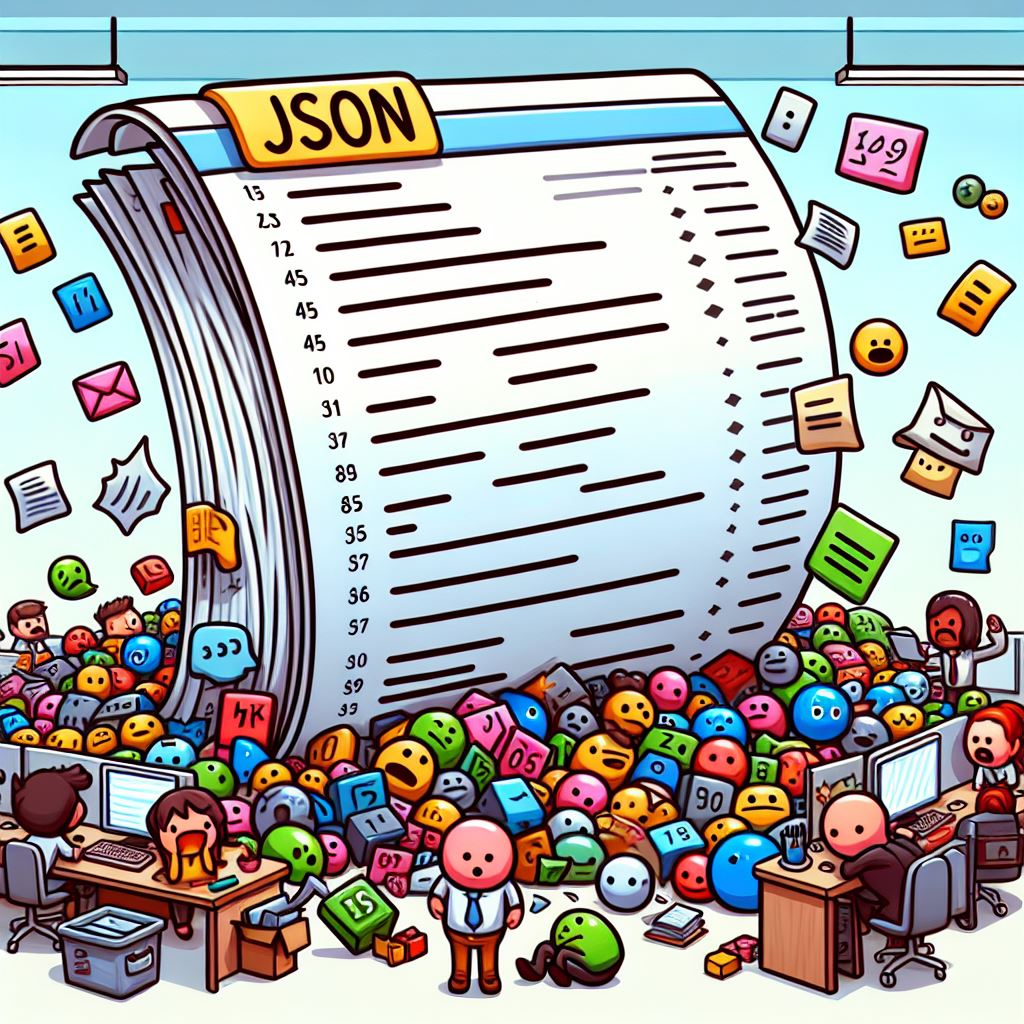
\includegraphics[width=3.2cm]{image/json-changing}
        \end{center}
    \end{frame}

    \begin{frame}[fragile]{Les objets}{JSON \lstinline{parse} et \lstinline{stringify}}
        \begin{footnotesize}
            L'objet \lstinline{JSON} porte deux méthodes utiles pour transformer une chaîne de caractère en JSON et inversement~:
            \begin{itemize}
                \item \lstinline{parse}~: Transforme une chaîne de caractère en JSON~.
                Utilisé pour \textquote{charger} un JSON stocké ou transféré.
                \begin{lstlisting}[language=Bash,title={\tiny{Node.js}},basicstyle=\tiny\ttfamily]
> JSON.parse('{"nom":"Adrien","age":25,"JavaScript":{"notes":[12,15,18],"Appréciation":"Excellent"},"CSS":{"notes":[10,14,16],"Appréciation":"Bon"}}')
{
  nom: 'Adrien',
  age: 25,
  JavaScript: { notes: [ 12, 15, 18 ], 'Appréciation': 'Excellent' },
  CSS: { notes: [ 10, 14, 16 ], 'Appréciation': 'Bon' }
}
                \end{lstlisting}
                \item \lstinline{stringify}~: Transforme un JSON en chaîne de caractère.
                Utile pour utiliser en JavaScript un JSON stocker dans un fichier ou réceptionné sur le réseau.
                \begin{lstlisting}[language=Bash,title={\tiny{Node.js}},basicstyle=\tiny\ttfamily]
> JSON.stringify(adrien)
'{"nom":"Adrien","age":25,"JavaScript":{"notes":[12,15,18],"Appréciation":"Excellent"},"CSS":{"notes":[10,14,16],"Appréciation":"Bon"}}'
                \end{lstlisting}
            \end{itemize}
        \end{footnotesize}
    \end{frame}

    \begin{frame}{JSON}{Exercice \execcounterdispinc{}}
        À l'aide de l'objet JSON \lstinline{adrien} et de la fonction \lstinline{mean} des slides précédents~:
        \begin{itemize}
            \item Calculer la moyenne des notes de JavaScript et de CSS~.
            \item Ajouter ces moyennes à l'objet \lstinline{adrien}~.
            \item Supprimer les notes de JavaScript et de CSS de l'objet \lstinline{adrien}~.
        \end{itemize}
        \bigbreak
        \centering
        
\includegraphics[width=3cm]{image/intelligence}
    \end{frame}

    \begin{frame}{Créer ses classes ou types d'objet}
        \begin{footnotesize}
            JavaScript est un langage orienté objet, comme tout ceux de cette catégorie, il permet de créer des classes.
            \bigbreak
            \begin{columns}
                \column{0.75\textwidth}
                \begin{itemize}
                    \item Une classe permet de créer des objets en les instanciant ou non avec des paramètres, passés à ceux qu'on appelle le \textquote{constructeur}.
                    \item Tout comme le JSON c'est une représentation abstraite d'un objet réel.
                    \item Il peut lui aussi porter des données
                    \item Mais il peut en plus porter des méthodes, des fonctions qui agissent sur les données ou sur le programme.
                    \item Un objet peut \textquote{hériter} d'un autre pour avoir les mêmes propriétés et donc réduire les développements.
                    \item Une classe \textquote{encapsule} ce dont elle est responsable, ce qui est reconnu pour aider à la lecture du code.
                \end{itemize}
                \column{0.25\textwidth}
                \centering
                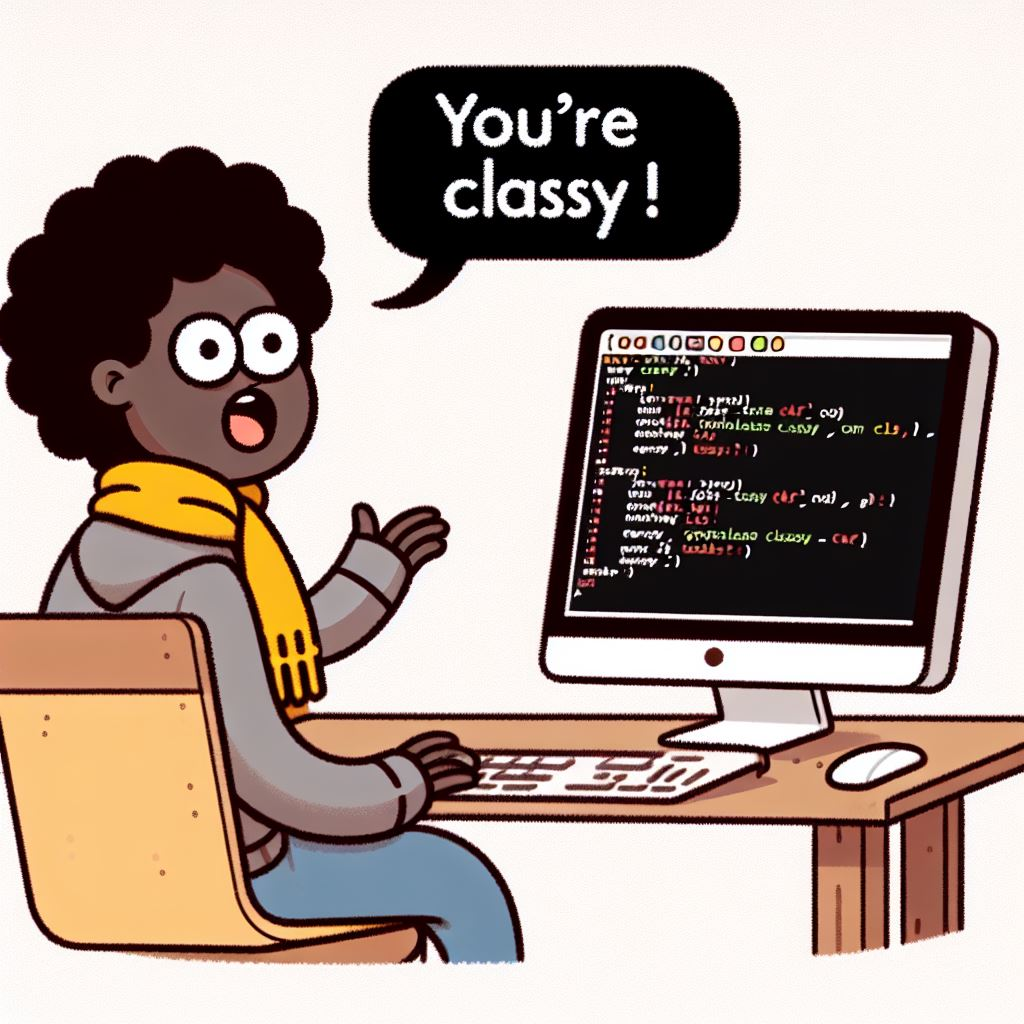
\includegraphics[width=3cm]{image/you-are-classy}
            \end{columns}
        \end{footnotesize}
    \end{frame}

    \begin{frame}[fragile]{Créer ses classes ou types d'objet}{Le constructeur}
        \begin{footnotesize}
            Le constructeur se déclare dans la classe avec le mot-clé \lstinline{constructor}.
            \begin{lstlisting}[language=JavaScript,title={\tiny{Script JavaScript}},basicstyle=\tiny\ttfamily]
class Car {

    static getFactoryWheelNumber() {
        return 4;
    }

    // Le bloc de code ci-dessous est le constrcuteur
    constructor(brand) {
        this.brand = brand;
        this.wheel = Car.getFactoryWheelNumber();
    }

    getCurrentWheelNumber() {
        return this.wheel;
    }
}
let myCar = new Car("Renault");
console.log(myCar.brand); // Renault
            \end{lstlisting}
            Le constructeur a un paramètre, la marque de la voiture.
            Le constructeur initialise la marque et le nombre de roues dans les propriétés préfixées par \lstinline{this}, propriétés propres à cette instance de la classe uniquement.
        \end{footnotesize}
    \end{frame}

    \begin{frame}[fragile]{Créer ses classes ou types d'objet}{Le constructeur}
        \begin{footnotesize}
            Deux instances d'une même classe ont bien des propriétés indépendantes.
            \begin{lstlisting}[language=JavaScript,title={\tiny{Script JavaScript}},basicstyle=\tiny\ttfamily]
class Car {

    static getFactoryWheelNumber() {
        return 4;
    }

    // Le bloc de code ci-dessous est le constrcuteur
    constructor(brand) {
        this.brand = brand;
        this.wheel = Car.getFactoryWheelNumber();
    }

    getCurrentWheelNumber() {
        return this.wheel;
    }
}
function carAccident(car) {
    car.wheel = 3;
}
let renault = new Car("Renault");
let mercedes = new Car("Mercedes");
carAccident(renault);
console.log("La Renautl a " + renault.wheel + " roues"); // 3 roues
console.log("La Mercedes a " + mercedes.wheel + " roues"); // 4 roues
            \end{lstlisting}
        \end{footnotesize}
    \end{frame}

    \begin{frame}[fragile]{Créer ses classes ou types d'objet}{Le constructeur}
        Donne en sortie~:
        \begin{lstlisting}[language=Bash,title={\tiny{Commande dans un Shell/Console/PowerShell}}]
La Renautl a 3 roues
La Mercedes a 4 roues
        \end{lstlisting}
        Expliquer pourquoi~?
        \bigbreak
        \begin{center}
            
\includegraphics[width=3cm]{image/intelligence}
        \end{center}
    \end{frame}


    \begin{frame}[fragile]{Créer ses classes ou types d'objet}{Le constructeur}
        \begin{footnotesize}
            Un constructeur n'a pas nécessairement d'argument.
            Si les propriétés de l'instance peuvent-être générées par le navigateur ou un appel d'API, quelque chose d'extérieur au programme et donc ne sont pas à passer en paramètre.
        \end{footnotesize}
        \begin{lstlisting}[language=JavaScript,title={\tiny{Script JavaScript}},basicstyle=\tiny\ttfamily]
class BrowserTracking {
    static geolocationSuccess(resolve, position) { resolve(position); }
    static geolocationError(reject, err) { reject(null); }
    static getPosition() {
        return new Promise((resolve, reject) => {
            navigator.geolocation.getCurrentPosition(
                BrowserTracking.geolocationSuccess.bind(null, resolve),
                BrowserTracking.geolocationError.bind(null, reject)
            );
        });
    }
    constructor() {
        this.agent = window.navigator.userAgent;
        this.screen = window.screen;
        BrowserTracking.getPosition().then(position => {
            this.position = position;
        }).catch(err => {
            this.position = err;
        });
    }
}
        \end{lstlisting}
    \end{frame}

    \begin{frame}{Créer ses classes ou types d'objet}{Le constructeur}
        \centering
        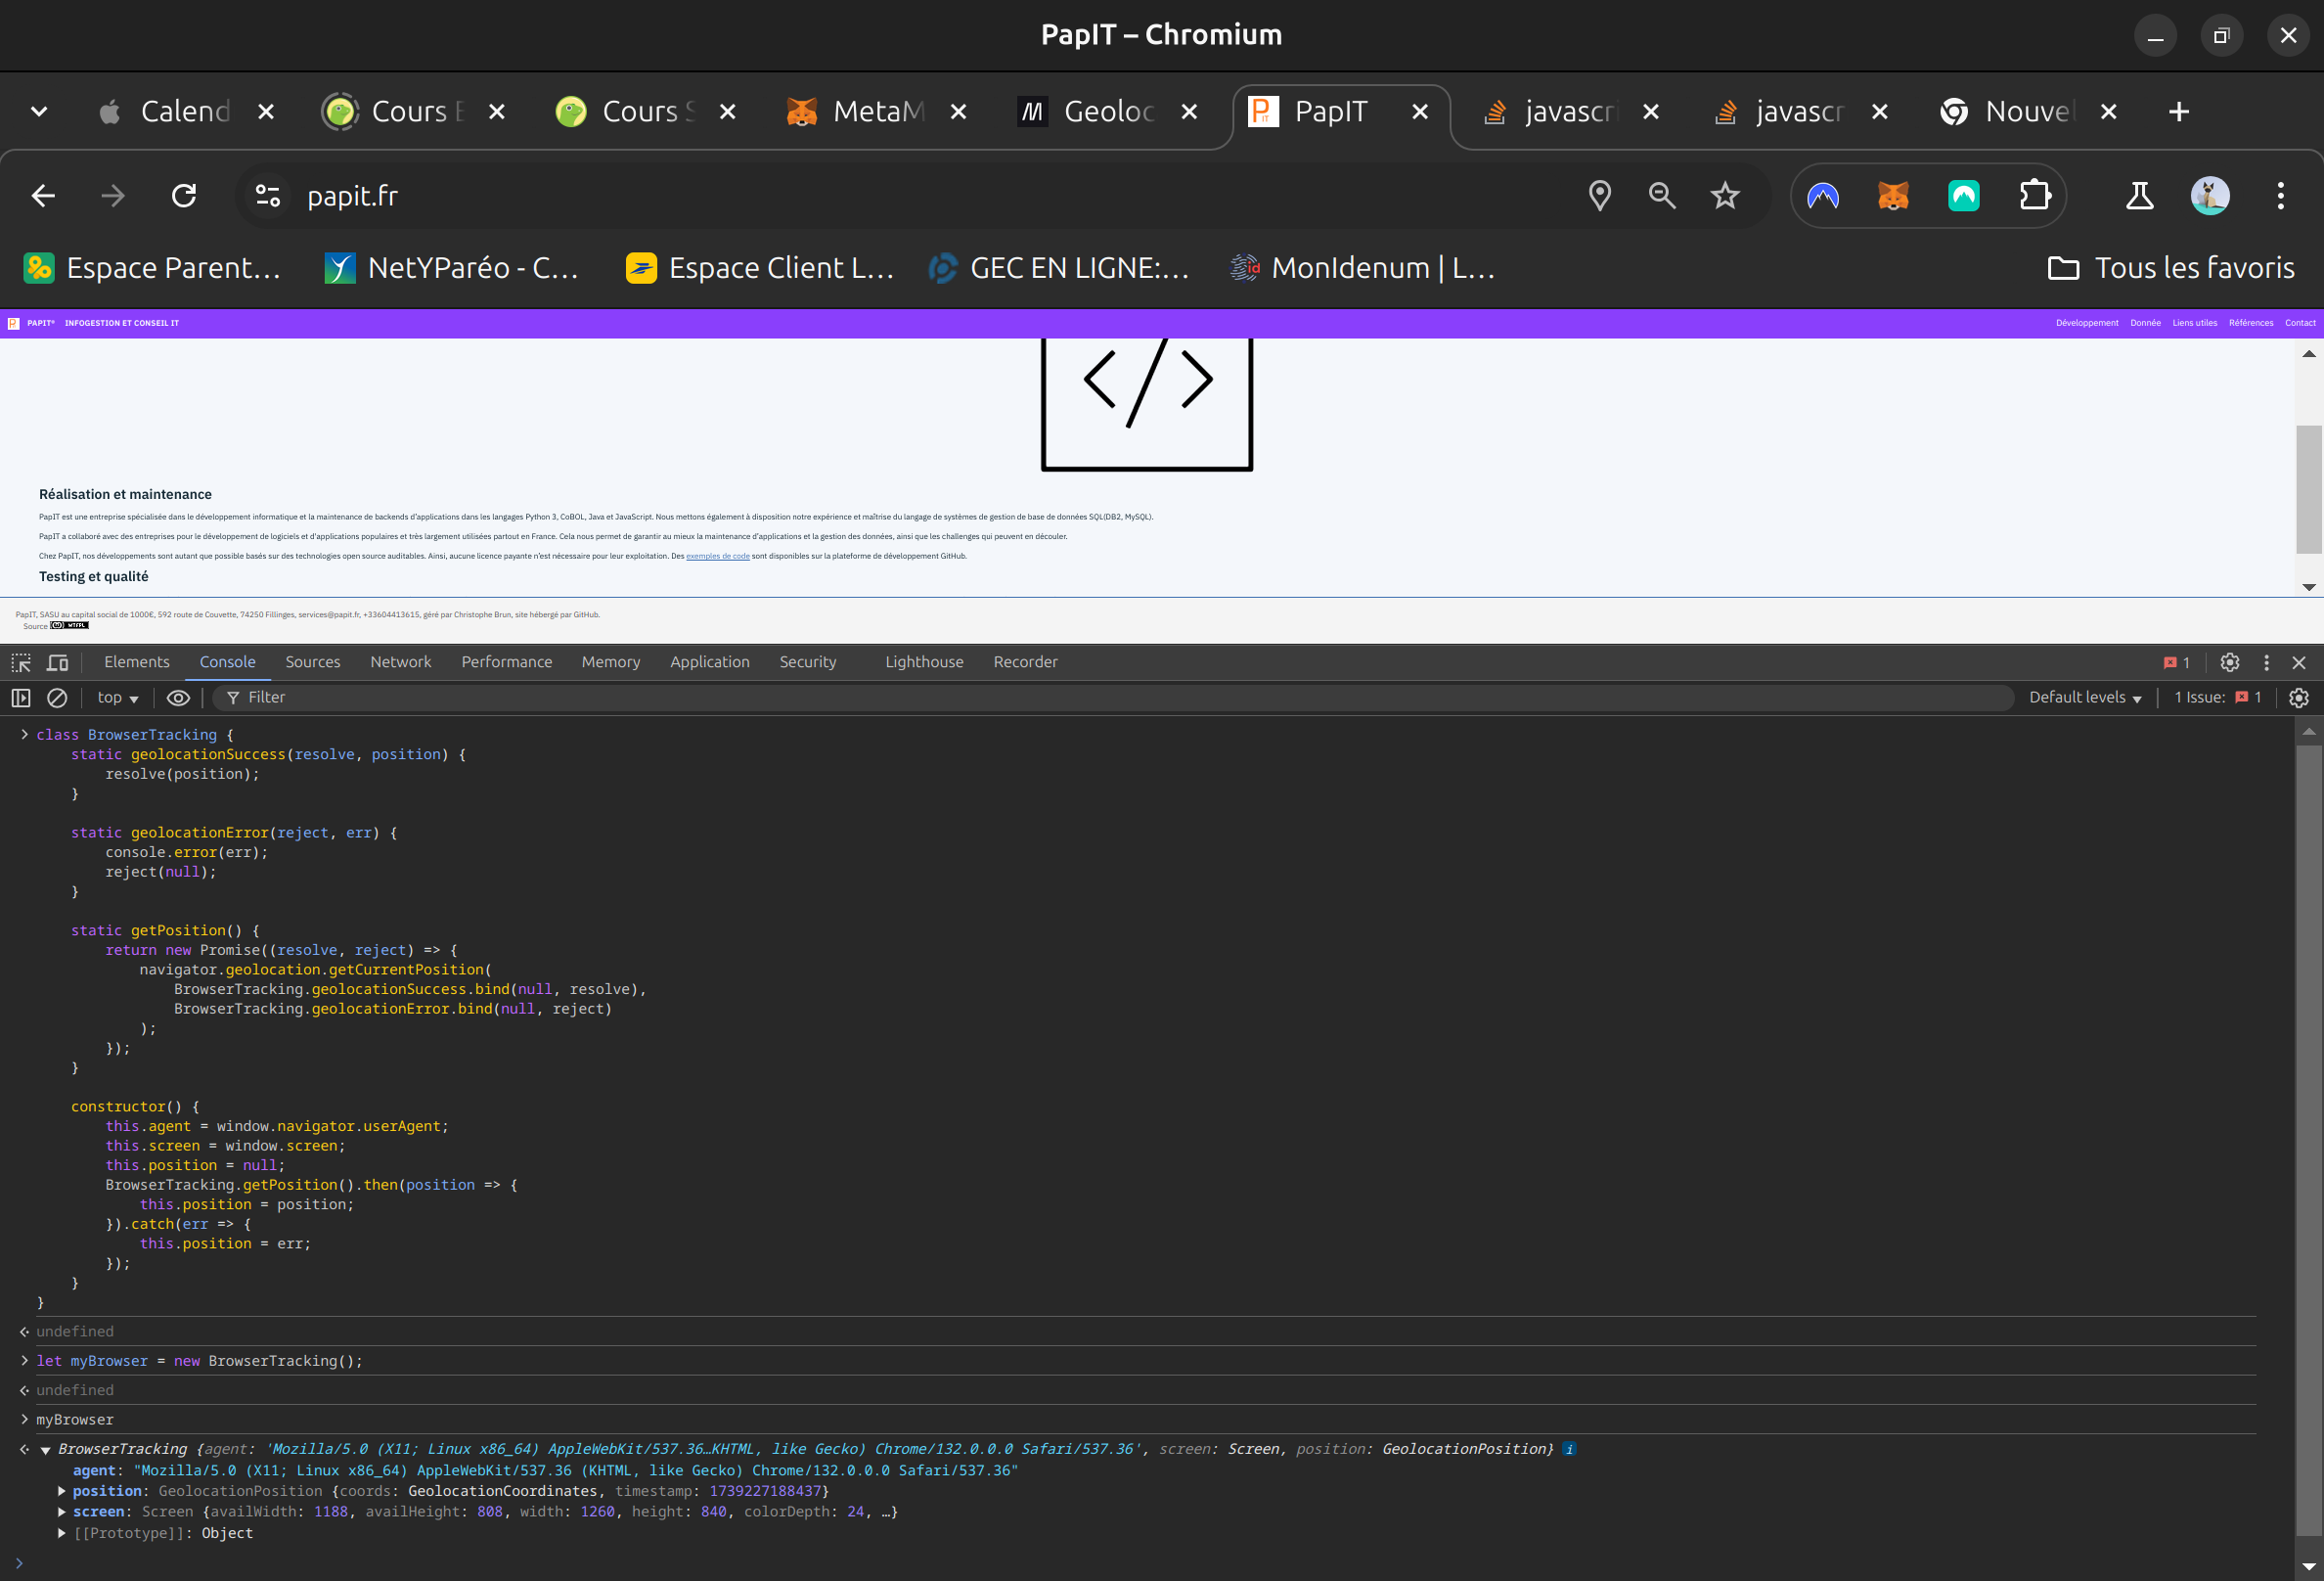
\includegraphics[width=11cm]{image/browser-tracker}
    \end{frame}


    \begin{frame}[fragile]{Créer ses classes ou types d'objet}{Les méthodes}
        \begin{footnotesize}
            Une méthode est une fonction qui agit grâce/sur les propriétés de l'objet.
            Exemple ici de la méthode \lstinline{isPrime}~:
            \begin{lstlisting}[language=JavaScript,title={\tiny{Script JavaScript}},basicstyle=\tiny\ttfamily]
class MDSNumber {
    constructor (integer) {
        this.integer = integer
    }
    isPrime() {
        if (this.integer < 2) {
            return false;
        }
        for (let i = 2; i <= Math.sqrt(this.integer); i++) {
            if (this.integer % i === 0) {
                return false;
            }
        }
        return true;
    }
}
            \end{lstlisting}
            \lstinline{isPrime} utilise la propriété \lstinline{integer} de l'instance de classe pour savoir si c'est un nombre premier.
            C'est donc bien une méthode.
        \end{footnotesize}
    \end{frame}

    \begin{frame}[fragile]{Créer ses classes ou types d'objet}{Les fonctions}
        \begin{footnotesize}
            Une fonction dîte statique, préfixée par \lstinline{static} en JS~.
            Exemple ici des fonctions \lstinline{mean} et \lstinline{factorial} qui n'utilisent pas de propriété de l'instance (même pas de constructeur)~:
            \begin{lstlisting}[language=JavaScript,title={\tiny{Script JavaScript}},basicstyle=\tiny\ttfamily]
class MathUtilities {
    // Static method to calculate the square of a number
    static mean(numbers) {
        let sum = 0;
        for (let i = 0; i < numbers.length; i++) {
            sum += numbers[i];
        }
        return sum / numbers.length;
    }
    static factorial(number) {
        if (number === 0) {
            return 1;
        }
        return number * MathUtilities.factorial(number - 1)
    }
}
console.log(MathUtilities.mean([1,2,3,4])); // Output 2.5
console.log(MathUtilities.factorial(5)); // Output 120
            \end{lstlisting}
            Cette classe, à l'image de la classe \lstinline{Math}, ne fait que encapsuler des fonctions mathématiques.
            Une classe peut évidement avoir des méthodes et des fonctions.
        \end{footnotesize}
    \end{frame}

    \begin{frame}[fragile]{Créer ses classes ou types d'objet}{L'héritage}
        \begin{footnotesize}
            Si un objet \textbf{est} également un autre objet (conceptuellement), il doit pouvoir hériter de ce dernier.
            Ici avec une corde d'escalade qui est aussi une corde et en hérite donc~:
            \begin{lstlisting}[language=JavaScript,title={\tiny{Script JavaScript}},basicstyle=\tiny\ttfamily]
class Corde{
    constructor(longueur){
        this.longueur = longueur
    }
    coupe(longueur){
        this.longueur -= longueur
    }
}
// extends est l'instruction qui soécifie la classe héritée
class CordeEscalade extends Corde {
    constructor(longueur){
        super(longueur) // super est l'instruction qui instancie la classe mère
    }
    longueurMax(poids){
        return this.longueur + (this.longueur * poids / 1000)
    }
}
let cordeEscalade = new CordeEscalade(100)
console.log(cordeEscalade.coupe(10)) // A les propriétés d'une corde
console.log(cordeEscalade.longueurMax(10)) // Et également d'une corde d'escalade
            \end{lstlisting}
            Par opposition un objet \textbf{a} des propriétés, comme ici la longueur, on parle de \textit{composition} de l'objet.
        \end{footnotesize}
    \end{frame}


    \begin{frame}{Créer ses classes ou types d'objet}{Exercice \execcounterdispinc{}}
        Développer une classe \lstinline{Chatter} qui permet de stocker des messages et de les afficher à l'avenir.
        \begin{itemize}
            \item La classe doit avoir un constructeur qui prend 2 paramètres, une chaîne de caractère \lstinline{nickname} et un entier nommé \lstinline{id}.
            Il initialise un tableau vide de messages.
            \item Une méthode qui retourne tous les messages.
            \item Une méthode qui retourne les 5 derniers messages avec \lstinline{slice}.
            \item Une méthode qui permet l'ajout d'un message.
            \item Une méthode qui ramène toutes les informations.
        \end{itemize}
        \bigbreak
        \centering
        
\includegraphics[width=3cm]{image/intelligence}
    \end{frame}


    \section{BOM (Browser Object Model)}\label{sec:bom}

    \begin{frame}{Introduction au Browser Object Model (BOM) et à l’objet Window\footnote{\label{giraud-js}Cours complet JavaScript, Pierre Giraud, \url{https://www.pierre-giraud.com/javascript-apprendre-coder-cours/browser-object-model-window/}}}
        \begin{footnotesize}
            Le BOM est une sorte de \textquote{super API} elle-même composée de plusieurs API dont certaines sont elles-mêmes composées de plusieurs API et \textit{etc}.
            \bigbreak
            À la base du BOM, nous avons l’interface \lstinline{Window} qui représente une fenêtre de navigateur contenant une page ou un document.
            \bigbreak
            Dans un navigateur utilisant des onglets, comme Firefox, chaque onglet contient son propre objet \lstinline{Window}.
            \bigbreak
            Cet objet \lstinline{Window} est un objet dit \textquote{implicite}~: Pas besoin de le mentionner de manière explicite pour utiliser les méthodes (ou fonctions globales) et propriétés (ou variables globales) lui appartenant.
            \bigbreak
            Le BOM est composé de différentes interfaces qu’on va pouvoir utiliser via des objets.
        \end{footnotesize}
    \end{frame}

    \begin{frame}{Les objets du BOM\cref{giraud-js}}
        Les objets suivants appartiennent au BOM et sont tous des enfants de \lstinline{Window}~:
        \begin{itemize}
            \item L’objet \lstinline{Navigator} qui représente l’état et l’identité du navigateur et qu’on va utiliser avec l’API Geolocation.
            L'objet instancié est \lstinline{navigator} ou \lstinline{window.navigator}.
            \item L’objet \lstinline{History} qui permet de manipuler l’historique de navigation du navigateur.
            L'objet instancié est \lstinline{history} ou \lstinline{window.history}.
            \item L’objet \lstinline{Location} qui fournit des informations relatives à l’URL de la page courante.
            L'objet instancié est \lstinline{location} ou \lstinline{window.location}.
            \item L’objet \lstinline{Screen} qui nous permet d’examiner les propriétés de l’écran qui affiche la fenêtre courante.
            L'objet instancié est \lstinline{screen} ou \lstinline{window.screen}.
            \item L’objet \lstinline{Document} et le DOM dans son ensemble que nous étudierons en détail dans la suite.
            C'est ce qui permet de modifier les balises HTML donc le rendu visuel du frontend.
            L'objet instancié est \lstinline{document} ou \lstinline{window.document}.
        \end{itemize}
    \end{frame}

    \begin{frame}{Les objets du BOM}{Les objets de \lstinline{window}}
        \centering
        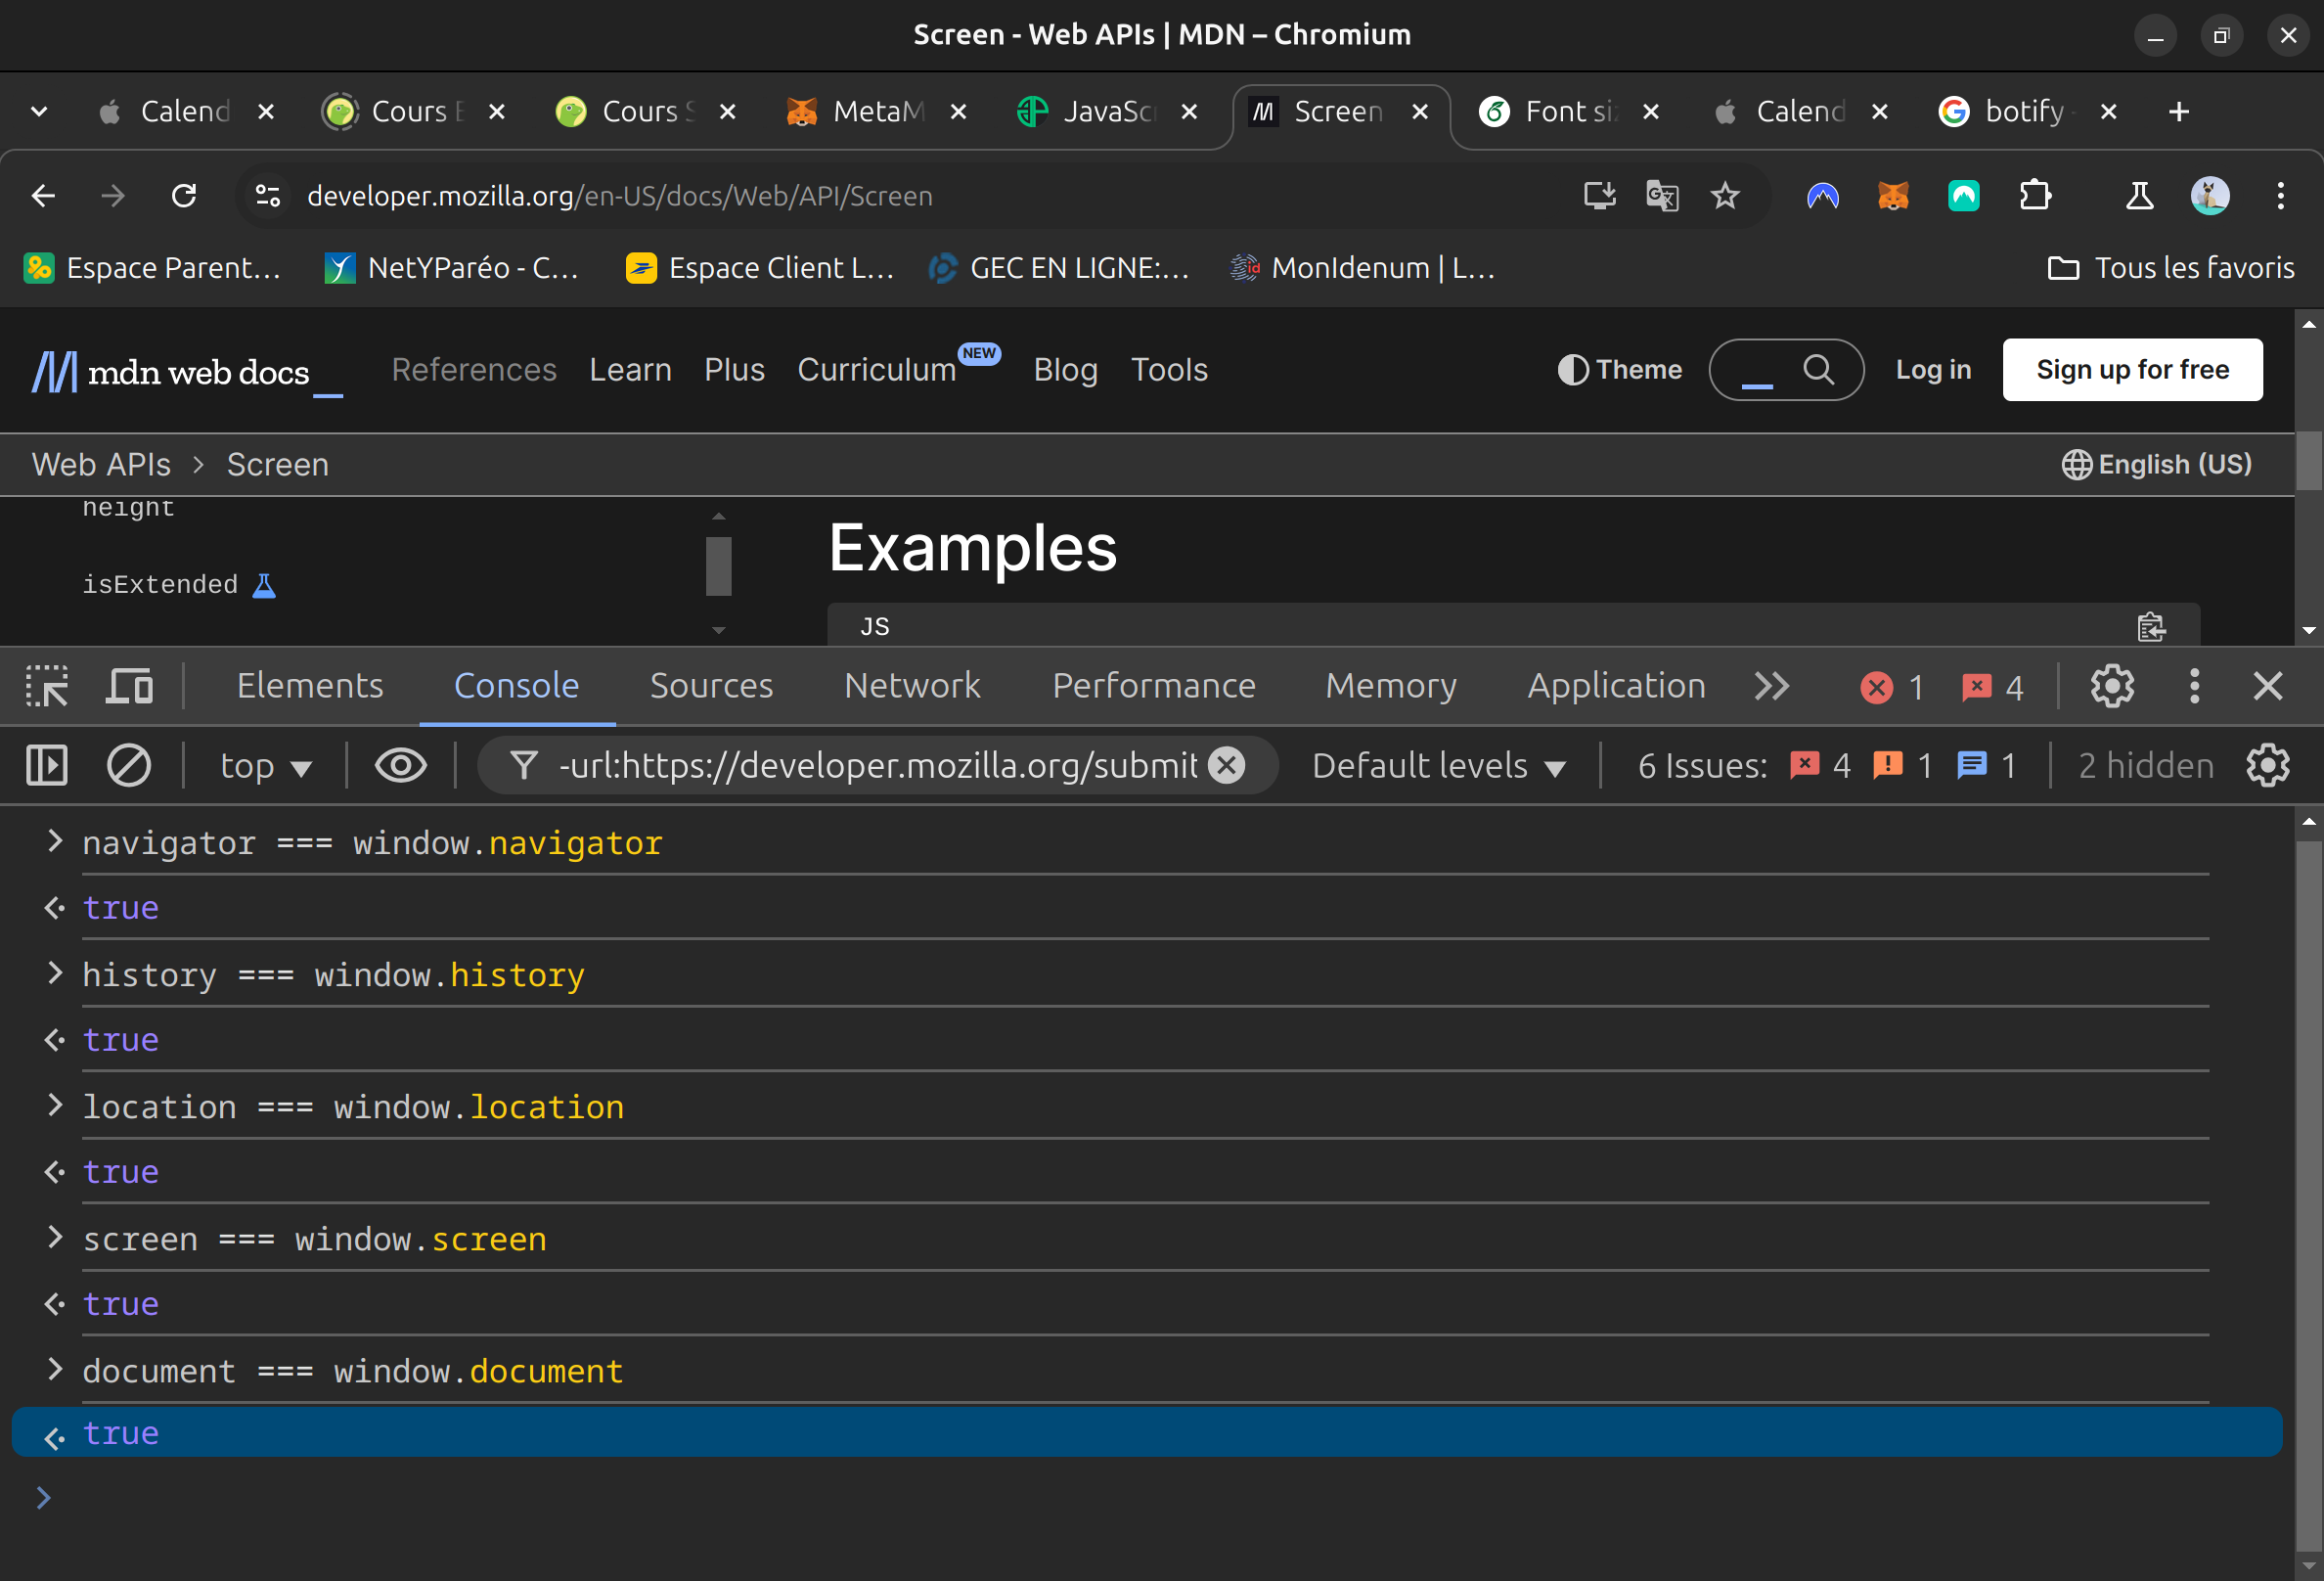
\includegraphics[width=9cm]{image/browser-window-objects}
        \flushleft
        C'est pour cela qu'on peut dire que \lstinline{window} est implicite, il n'est pas écrit pour gagner en temps de rédaction et lisibilité du code.
    \end{frame}

    \begin{frame}{Les objets du BOM}{Les objets de \lstinline{window}}
        \centering
        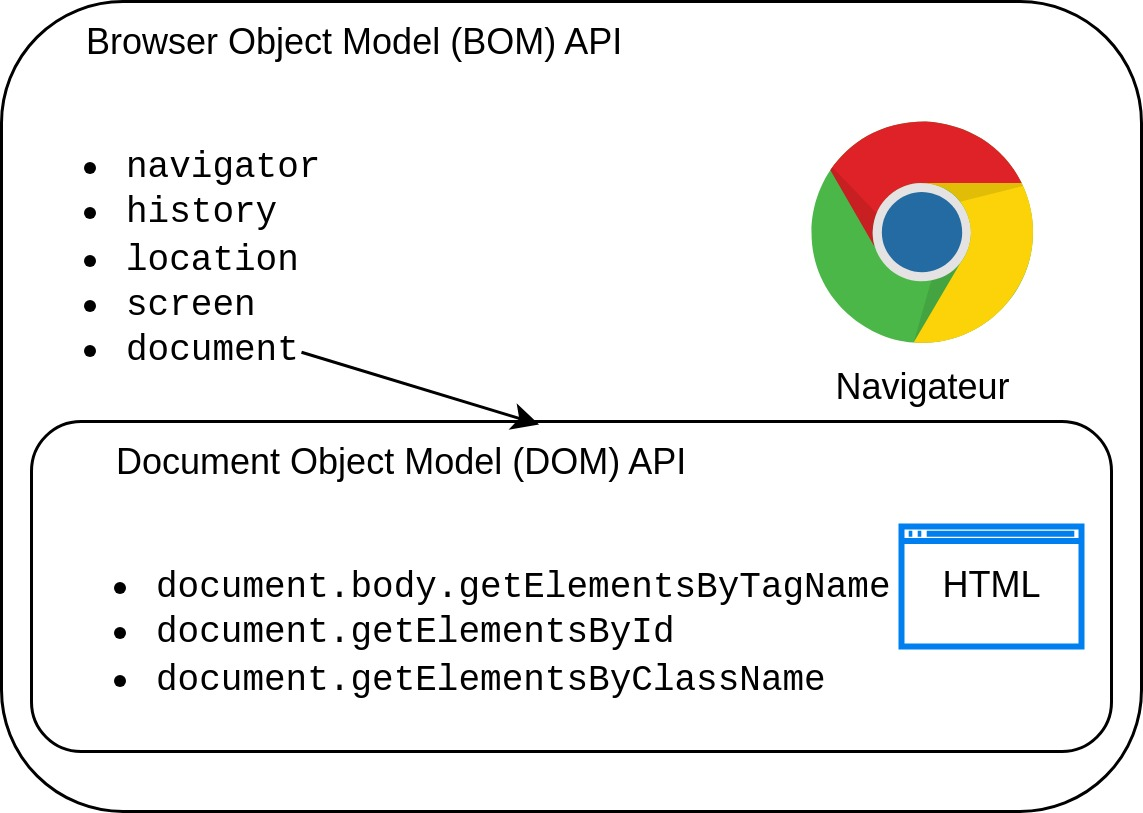
\includegraphics[width=10cm]{image/bom-n-dom}
    \end{frame}

    \subsection{L'objet navigator}\label{subsec:navigator}

    \begin{frame}{Les objets du BOM}{L'objet \lstinline{navigator}}
        L'objet \lstinline{navigator} porte de nombreuses données et méthodes sur la machine sur laquelle tourne le navigateur, le navigateur lui-même, la géolocalisation supposée, \textit{etc}.
        \bigbreak
        Exercice \execcounterdispinc{}~:
        \begin{itemize}
            \item Découvrir l'objet \lstinline{navigator} dans la console du navigateur.
            \item Découvrir le fonctionnement de la méthode \lstinline{getCurrentPosition} (\url{https://developer.mozilla.org/en-US/docs/Web/API/Geolocation/getCurrentPosition}) et la faire fonctionner dans la console du navigateur.
            \item En s'inspirant de la vue précédemment, ajouter la latitude et la longitude à l'objet \lstinline{Chatter} de l'exercice précédent.
        \end{itemize}
    \end{frame}

    \subsection{L'objet location}\label{subsec:location}

    \begin{frame}{Les objets du BOM}{L'objet \lstinline{location}}
        \begin{tiny}
            L'objet \lstinline{location} porte de nombreuses données et méthodes, l'URL en cours de navigation, le rechargement de l'URL, le changement d'URL (de page), \textit{etc}.
            \bigbreak
            Exercice \execcounterdispinc{}~:
            \begin{itemize}
                \item Découvrir l'objet \lstinline{location} dans la console du navigateur.
                \item Découvrir le fonctionnement de la méthode \lstinline{replace} (\url{https://developer.mozilla.org/fr/docs/Web/API/Location/replace}) et la faire fonctionner dans la console du navigateur.
                \item Découvrir le fonctionnement de la méthode \lstinline{reload} (\url{https://developer.mozilla.org/fr/docs/Web/API/Location/reload}) et la faire fonctionner dans la console du navigateur.
                \item Comment utiliser \lstinline{location} pour lier une adresse à une donnée dans une base de donnée~?
                \item Ajouter au constructeur de la classe \lstinline{Chatter} de l'exercice précédent, une propriété \lstinline{origine} qui est le nom du serveur, c'est-à-dire, le \lstinline{hostname}.
                \item Modifier au besoin méthode qui ajoute les messages de \lstinline{Chatter} pour qu'ils aient comme propriétés~:
                \begin{itemize}
                    \begin{tiny}
                        \item \lstinline{message}~: Le message en lui-même, une chaîne de caractère.
                        \item \lstinline{date}~: La date de l'ajout du message, un objet \lstinline{Date}.
                        \item \lstinline{id}~: Un identifiant unique généré avec \lstinline{Math.random().toString(16).slice(2)}.
                    \end{tiny}
                \end{itemize}
                \item Ajouter à \lstinline{Chatter} une méthode qui permet de retourner un message par son \lstinline{id}.
                \item Tester cela dans un script ajouté à un page HTML et tenter de retourner des messages par leur \lstinline{id}.
                Tester également quand l'\lstinline{id} est incorrect.
            \end{itemize}
        \end{tiny}
    \end{frame}

    \subsection{L'objet history}\label{subsec:history}

    \begin{frame}{Les objets du BOM}{L'API \lstinline{history}\footnote{\label{history}Manipuler l'historique du navigateur, \url{https://developer.mozilla.org/fr/docs/Web/API/History_API}}}
        L'API History permet de manipuler l'historique de navigation du navigateur.
        Les méthodes principales sont:
        \begin{itemize}
            \item \lstinline{back()}, équivaut à cliquer sur le bouton \textquote{précédent} du navigateur.
            \item \lstinline{forward()}, équivaut à cliquer sur le bouton \textquote{suivant} du navigateur.
            \item \lstinline{go()}, pour aller à une page spécifique de l'historique.
            \item \lstinline{pushState()}, pour ajouter une entrée à l'historique.
            \item \lstinline{replaceState()}, pour modifier l'entrée actuelle de l'historique.
        \end{itemize}
        \bigbreak
        Cette API permet d'améliorer l'impression de navigation dans une seule et même page, sans en changer.
        Par exemple sur un application de streaming de musique, si on changeait de page en navigant, la lecture s'interromprait.
        Cette API de revenir en arrière, modifier l'historique, sans avoir changé de page.
    \end{frame}

    \begin{frame}[fragile]{Les objets du BOM}{Méthode \lstinline{back()} de l'API \lstinline{history}\cref{history}}
        La méthode \lstinline{back()} permet de reculer d'une page dans l'historique de navigation.
        \begin{lstlisting}[language=JavaScript,title={\tiny{Script JavaScript}}]
window.history.back();
        \end{lstlisting}
        Équivaut à cliquer sur le bouton \textquote{précédent} du navigateur.
        \begin{center}
            
\includegraphics[width=3cm]{image/page-first}
        \end{center}
    \end{frame}

    \begin{frame}[fragile]{Les objets du BOM}{Méthode \lstinline{forward()} de l'API \lstinline{history}\cref{history}}
        La méthode \lstinline{forward()} permet d'avancer d'une page dans l'historique de navigation.
        \begin{lstlisting}[language=JavaScript,title={\tiny{Script JavaScript}}]
window.history.forward();
        \end{lstlisting}
        Équivaut à cliquer sur le bouton \textquote{suivant} du navigateur.
        \begin{center}
            
\includegraphics[width=3cm]{image/page-last}
        \end{center}
    \end{frame}

    \begin{frame}[fragile]{Les objets du BOM}{Méthode \lstinline{go()} de l'API \lstinline{history}\cref{history}}
        La méthode \lstinline{go()} permet de naviguer vers une page spécifique de l'historique en utilisant un index relatif.
        L'argument à passer est un entier, l'index dans l'historique.
        \begin{lstlisting}[language=JavaScript,title={\tiny{Script JavaScript}}]
window.history.go(-1); // Reculer d'une page
window.history.go(1);  // Avancer d'une page
        \end{lstlisting}
    \end{frame}

    \begin{frame}[fragile]{Les objets du BOM}{Événement \lstinline{popstate} de l'API \lstinline{history}\cref{history}}
        L'événement \lstinline{popstate} est déclenché lorsque l'entrée active de l'historique change.
        Il est généré par l'élément \lstinline{window} et prend en second argument l'action à réaliser lorsque l'élément est déclenché.
        \begin{lstlisting}[language=JavaScript,title={\tiny{Script JavaScript}}]
window.addEventListener('popstate', (event) => {
    console.log('location: ' + document.location + ', state: ' + JSON.stringify(event.state));
});
        \end{lstlisting}
    \end{frame}

    \begin{frame}[fragile]{Les objets du BOM}{Méthode \lstinline{pushState()} de l'API \lstinline{history}\cref{history}}
        La méthode \lstinline{pushState()} ajoute une entrée à l'historique de navigation.
        \begin{lstlisting}[language=JavaScript,title={\tiny{Script JavaScript}}]
window.history.pushState({page: 1}, 'title 1', '?page=1');
        \end{lstlisting}
        \begin{itemize}
            \item Le premier paramètre est un objet qui représente l'état associé à l'entrée.
            \item Le second paramètre ne sert à rien, c'est un héritage garder pour ne pas casser des compatibilités.
            Il peut être une chaîne de caractères vide.
            \item Le troisième paramètre est le path d'une URL de la nouvelle entrée.
            Elle doit être sur le même domaine.
        \end{itemize}
    \end{frame}

    \begin{frame}[fragile]{Les objets du BOM}{Méthode \lstinline{replaceState()} de l'API \lstinline{history}\cref{history}}
        La méthode \lstinline{replaceState()} modifie l'entrée actuelle de l'historique, celle de la page en cours de navigation.
        \begin{lstlisting}[language=JavaScript,title={\tiny{Script JavaScript}}]
window.history.replaceState({page: 2}, 'title 2', '?page=2');
        \end{lstlisting}
        \begin{itemize}
            \item Le premier paramètre est un objet qui représente l'état associé à l'entrée.
            \item Le second paramètre ne sert à rien, c'est un héritage garder pour ne pas casser des compatibilités.
            Il peut être une chaîne de caractères vide.
            \item Le troisième paramètre est le path d'une URL de la nouvelle entrée.
            Elle doit être sur le même domaine.
        \end{itemize}
    \end{frame}

    \begin{frame}{Les objets du BOM}{Exercice \execcounterdispinc{}}
        Dans la classe \lstinline{Chatter} déclarée précédemment, modifier la méthode qu'il convient pour ajouter à l'historique de navigation les pages correspondants aux messages créés.
        \bigbreak
        \centering
        
\includegraphics[width=3cm]{image/intelligence}
    \end{frame}

    \subsection{L'object screen}\label{subsec:screen}

    \begin{frame}[fragile]{Les objets du BOM}{L'objet \lstinline{screen}}
        L'objet \lstinline{screen} porte de nombreuses données sur la taille de la fenêtre du navigateur.
        \bigbreak
        Exercice \execcounterdispinc{}~:
        \begin{itemize}
            \item Découvrir l'objet \lstinline{screen} dans la console du navigateur et \url{https://developer.mozilla.org/en-US/docs/Web/API/Screen}.
            \item Initialiser dans le constructeur de \lstinline{Chatter} un booléen \lstinline{isMobile} à \lstinline{true} si l'écran est celui d'un mobile, sinon à \lstinline{false}, à l'aide de l'objet \lstinline{screen}.
        \end{itemize}
        \begin{center}
            
\includegraphics[width=3cm]{image/intelligence}
        \end{center}
    \end{frame}


    \section{Document Object Model}\label{sec:dom}

    \subsection{Nœuds}\label{sucsec:nodes}

    \begin{frame}[fragile]{La DOM API}{Les nœuds\cref{eloquent-javaScript}}
        Chaque balise HTML peut être considérée comme un nœud parent ou/et enfant d'un autre.
        \bigbreak
        Ici \lstinline{html} est parent de \lstinline{head} et \lstinline{body}, \lstinline{body} est parent de \lstinline{h1} et \lstinline{p}, \textit{etc}.
        \begin{lstlisting}[language=HTML,title={\tiny{HTML}}]
<!doctype html>
<html>
  <head>
    <title>My home page</title>
  </head>
  <body>
    <h1>My home page</h1>
    <p>Hello, I am Marijn and this is my home page.</p>
    <p>I also wrote a book! Read it
      <a href="http://eloquentjavascript.net">here</a>.</p>
  </body>
</html>
        \end{lstlisting}
        Si on a un parent c'est que l'on est un enfant\ldots
    \end{frame}

    \begin{frame}{La DOM API}{Les nœuds\cref{eloquent-javaScript}}
        \begin{center}
            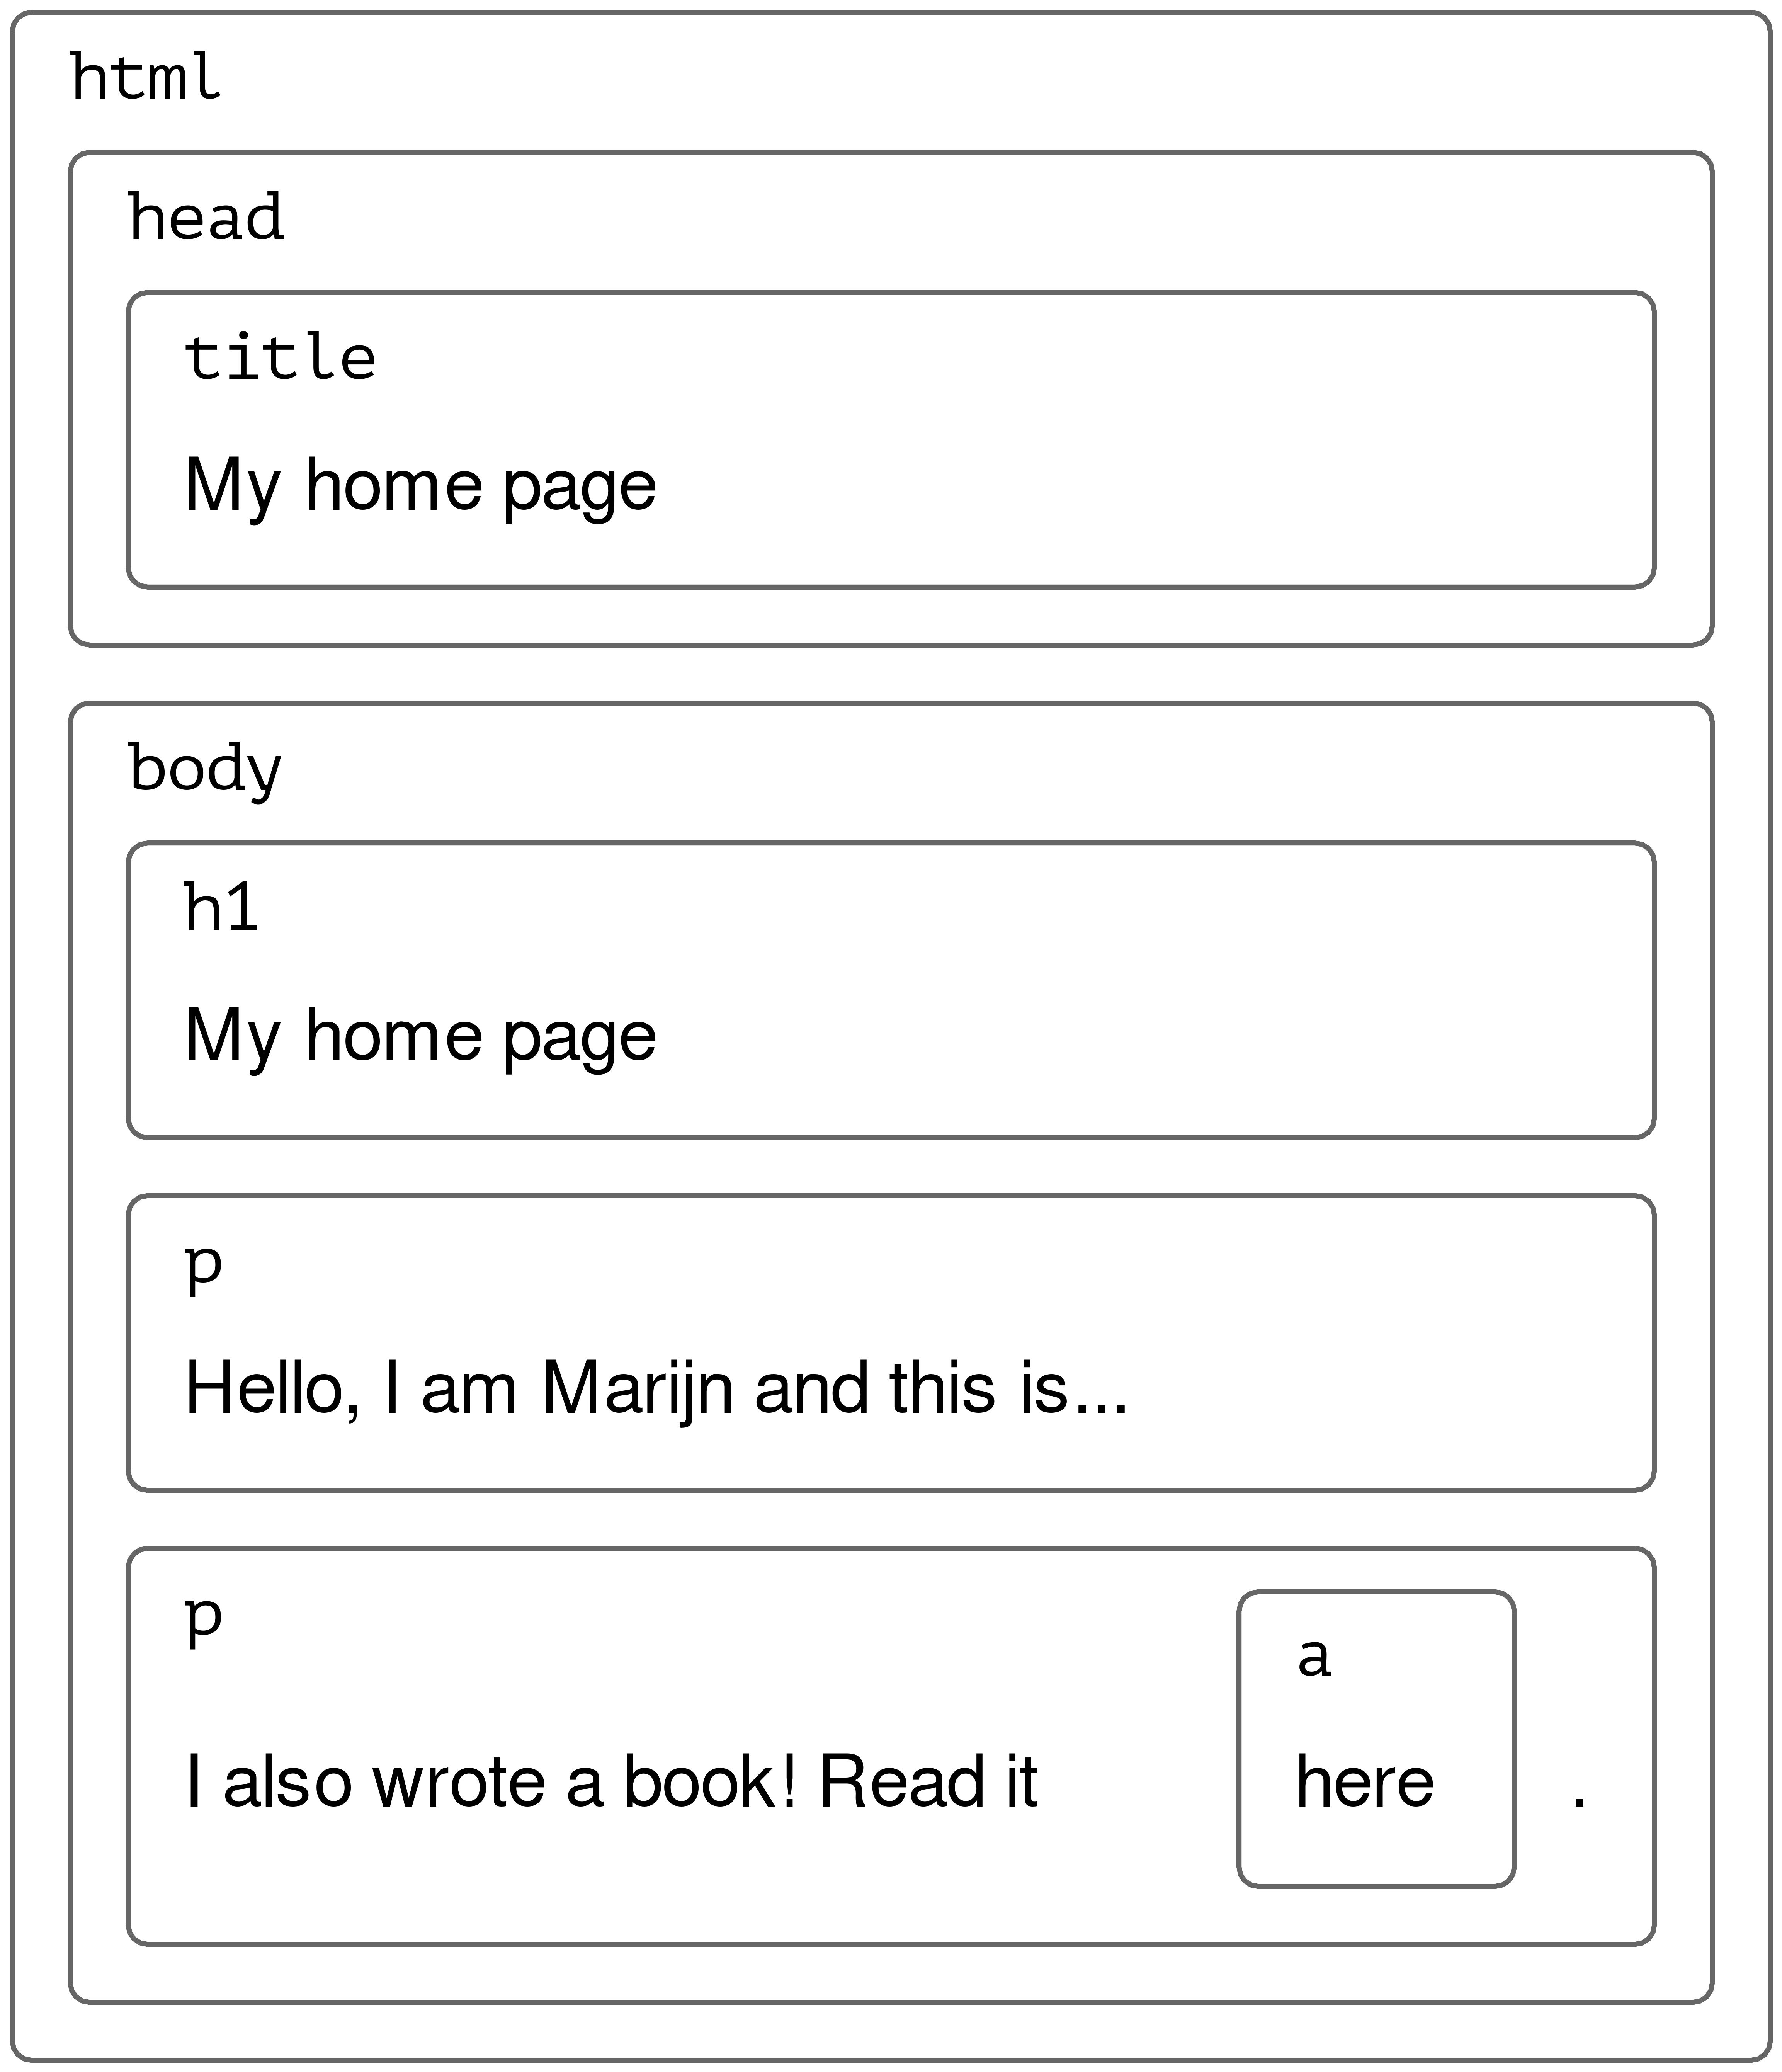
\includegraphics[width=6cm]{image/html-boxes}
        \end{center}
    \end{frame}

    \subsection{Trouver les élements (nœuds)}\label{subsec:elements}
    \begin{frame}{La DOM API}{Trouver les élements (nœuds)\cref{eloquent-javaScript}}
        Un nœud aussi appelé élement peut être retourné grâce aux méthodes de l'objet \lstinline{document}~:
        \begin{itemize}
            \item \lstinline{getElementById}~: Retourne l'élément avec l'identifiant donné.
            \item \lstinline{getElementsByTagName}~: Retourne une collection \lstinline{HTMLCollection} d'éléments avec le nom de balise donné.
            \item \lstinline{getElementsByClassName}~: Retourne une collection \lstinline{HTMLCollection} d'éléments avec la classe donnée.
            \item \lstinline{querySelector}~: Retourne le premier élément qui correspond au sélecteur CSS donné.
            \item \lstinline{querySelectorAll}~: Retourne tous les éléments qui correspondent au sélecteur CSS donné dans une collection \lstinline{HTMLCollection}.
        \end{itemize}
        \begin{dangercolorbox}
            \textbf{getElements} avec un \textbf{s} retourne une \lstinline{HTMLCollection}, \textbf{getElement} au singulier retourne un \lstinline{HTMLElement}
        \end{dangercolorbox}
    \end{frame}

    \begin{frame}[fragile]{La DOM API}{Trouver les élements (nœuds)\cref{eloquent-javaScript}}
        Une collection \lstinline{HTMLCollection} est un type proche des tableaux.
        Il est même possible de convertir une \lstinline{HTMLCollection} en \lstinline{Array} avec \lstinline{Array.from}, si nécessaire.
        \begin{lstlisting}[language=JavaScript,title={\tiny{Script JavaScript}}]
let paragraphs = Array.from(document.getElementsByTagName("p"))
        \end{lstlisting}
        Sinon \lstinline{HTMLCollection} ne supportent que la boucle for / of et non for / in par exemple.
        \begin{lstlisting}[language=JavaScript,title={\tiny{Script JavaScript}}]
for (let item of document.getElementsByTagName("p")) {
    console.log(item.id);
}
        \end{lstlisting}
    \end{frame}

    \begin{frame}{La DOM API}{Les propriétés d'un element\footnote{HTMLElement, \url{https://developer.mozilla.org/fr/docs/Web/API/HTMLElement}}}
        \begin{scriptsize}
            La \lstinline{HTMLCollection} est une collection d'objets \lstinline{HTMLElement}.
            Ils ont de (trop) nombreuses propriétés, les plus utiles sont~:
            \begin{itemize}
                \item \lstinline{innerHTML}~: Contenu HTML de l'élément.
                \item \lstinline{innerText}~: Contenu textuel de l'élément.
                \item \lstinline{style}~: Style CSS de l'élément.
                \item \lstinline{classList}~: Liste des classes de l'élément.
                \item \lstinline{dataset}~: Liste des attributs \lstinline{data-*} de l'élément.
                \item \lstinline{children}~: Liste des enfants de l'élément.
                \item \lstinline{parentElement}~: Parent de l'élément.
                \item \lstinline{hiden}~: Une valeur booléenne indiquant si l'élément est caché.
                \item \lstinline{title}~: Une chaîne de caractères contenant le texte apparaissant dans la bulle d'information affichée lorsque la souris survole l'élément.
                \item Bien, plus encore.
                Partez du principe que la propriété que vous cherchez existe.
                Il y a une propriété pour chaque attribut HTML~.
                Il faut aller lire la documentation pour la connaître.
            \end{itemize}
            \begin{dangercolorbox}
                Ces propriétés peuvent être \textbf{lues} et \textbf{écrites}.
            \end{dangercolorbox}
        \end{scriptsize}
    \end{frame}

    \begin{frame}{La DOM API}{Les méthodes d'un element}
        \begin{footnotesize}
            Les attributs et l'intérieur de la balise, que ce soit du texte ou un élément HTML enfant doivent pouvoir être créés/modifiés/supprimés.
            Pour cela des méthodes qui prennent des arguments comme la valeur à mettre ou l'élément à ajouter sont disponibles~:
            \begin{itemize}
                \item \lstinline{setAttribute}~: Ajoute un attribut à un élément.
                Prend comme paramètres, le nom de l'attribut suivit de sa valeur.
                \item \lstinline{removeAttribute}~: Supprime un attribut à un élément.
                \item \lstinline{appendChild}~: Ajoute un élément enfant à un l'élément.
                \item \lstinline{removeChild}~: Supprime un élément enfant à un l'élément.
                \item \lstinline{replaceChild}~: Remplace un élément enfant à un l'élément.
                \item \lstinline{insertBefore}~: Insère un élément avant un autre
                \item \lstinline{cloneNode}~: Clone un élément.
                \item \lstinline{remove}~: Supprime l'élément.
                \item \lstinline{getAttribute}~: Retourne la valeur de l'attribut donné.
                \item \lstinline{hasAttribute}~: Retourne un booléen indiquant si l'élément a l'attribut donné.
                \item \lstinline{querySelector}~: Retourne le premier élément qui correspond au sélecteur donné.
                \item \lstinline{querySelectorAll}~: Retourne tous les éléments qui correspondent au sélecteur donné dans une collection \lstinline{HTMLCollection}.
            \end{itemize}
        \end{footnotesize}
    \end{frame}

    \begin{frame}[fragile]{La DOM API}{Les évènement d'un élément}
        \begin{footnotesize}
            Un évènement peut être déclenché sous de multiples conditions, grâce aux \lstinline{EventListener}.
            Ils prennent en paramètre un évènement et l'action à y associer.
            \begin{itemize}
                \item Lorsque la page est chargée complètement.
                \begin{lstlisting}[language=JavaScript,title={\tiny{Script JavaScript}}]
document.addEventListener("DOMContentLoaded", function() {
    console.log("La page est chargée");
});
                \end{lstlisting}
                \item Lorsque l'input de l'élément d'un formulaire est modifié.
                \begin{lstlisting}[language=JavaScript,title={\tiny{Script JavaScript}}]
let name = document.getElementById("name");
name.addEventListener("input", function() {
    console.log("Le nom a été modifié");
});
                \end{lstlisting}
            \end{itemize}
        \end{footnotesize}
    \end{frame}

    \begin{frame}[fragile]{La DOM API}{Les évènement d'un élément}
        \begin{footnotesize}
            \begin{itemize}
                \item Lorsque la souris passe sur l'élément.
                \begin{lstlisting}[language=JavaScript,title={\tiny{Script JavaScript}}]
let name = document.getElementById("submit-button");
name.addEventListener("mouseover", function() {
    console.log("La souris est sur le bouton");
});
                \end{lstlisting}
                \item Lorsque l'élément est cliqué.
                \begin{lstlisting}[language=JavaScript,title={\tiny{Script JavaScript}}]
let name = document.getElementById("submit-button");
name.addEventListener("click", function() {
    console.log("Clique sur le bouton");
});
                \end{lstlisting}
                \item \ldots
            \end{itemize}
        \end{footnotesize}
    \end{frame}

    \begin{frame}{La DOM API}{Exercice \execcounterdispinc{}}
        Dans le HTML créé précédemment~:
        \begin{itemize}
            \item Importer une bibliothèque CSS comme Bootstrap, ou une autre que vous connaissez pour faciliter la mise en forme.
            \item Créer un formulaire qui a comme \textit{inputs} les champs nécessaires à l'initialisation du constructeur de \lstinline{Chatter}.
            \item Un bouton de soumission du formulaire qui n'a pas d'action définit dans le HTML~.
            \item Créer un bloque de code qui n'est exécuté que quand la page est chargée.
            \item Dans ce dernier bloque de code, ajouter un évènement sur le bouton de soumission qui récupère les valeurs des \textit{inputs} et initialise un nouvel objet \lstinline{Chatter}.
        \end{itemize}
    \end{frame}

    \begin{frame}{La DOM et BOM API}{Exercice \execcounterdispinc{}}
        Toujours dans le même HTML~:
        \begin{itemize}
            \item Utiliser \lstinline{location} pour récupérer, si il y en a un, le hash et l'utiliser comme identifiant de \lstinline{Chatter}.
            \item Le paramètre nom prend maintenant un argument par défaut, la chaîne de caractère \lstinline{anonyme}.
            \item Si il y a un hash, l'identifiant de \lstinline{Chatter} est ce hash et le nom celui, par défaut.
            \item Si il y a un hash, préremplir l'input identifiant du formulaire avec ce dernier.
            \item Modifier le titre du document pour qu'il contienne le nom de l'objet \lstinline{Chatter} quand il est renseigné, sinon, le hash.
        \end{itemize}
        \bigbreak
        \centering
        
\includegraphics[width=2cm]{image/intelligence}
    \end{frame}

    \begin{frame}{La DOM API}{Se déplacer dans l'arborescence\cref{eloquent-javaScript}}
        Un element porte de nombreuses propriétés pour se déplacer dans l'arborescence.
        \begin{columns}
            \column{0.7\textwidth}
            \begin{footnotesize}
                \begin{itemize}
                    \item \lstinline{parentNode}~: Parent de l'élément.
                    \item \lstinline{childNodes}~: Liste des enfants de l'élément.
                    \item \lstinline{firstChild}~: Premier enfant de l'élément.
                    \item \lstinline{lastChild}~: Dernier enfant de l'élément.
                    \item \lstinline{nextSibling}~: Élément suivant du parent, un nœud ou un élément texte.
                    \item \lstinline{previousSibling}~: Élément précédent du parent, un nœud ou un élément texte.
                    \item \lstinline{children}~: Liste des enfants de l'élément.
                    \item \lstinline{firstElementChild}~: Premier enfant de l'élément.
                    \item \lstinline{lastElementChild}~: Dernier enfant de l'élément.
                    \item \lstinline{nextElementSibling}~: Retourne toujours le nœud suivant du parent.
                    \item \lstinline{previousElementSibling}~: Retourne toujours le nœud précédent du parent.
                \end{itemize}
            \end{footnotesize}
            \column{0.3\textwidth}
            \center
            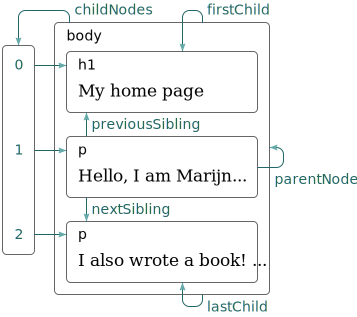
\includegraphics[width=4cm]{image/moving-in-the-tree}
        \end{columns}
    \end{frame}

    \begin{frame}[fragile]{La DOM API}{Modifier l'arborescence\cref{eloquent-javaScript}}
        \begin{tiny}
            Presque tout sur la structure de données DOM peut être modifié.
            La forme de l'arbre du document peut être modifiée en changeant les relations parent-enfant.
            Les nœuds ont une méthode \lstinline{remove} pour les retirer de leur nœud parent actuel.
            Pour ajouter un nœud enfant à un nœud élément, nous pouvons utiliser \lstinline{appendChild}, qui le place à la fin de la liste des enfants, ou \lstinline{insertBefore}, qui insère le nœud donné en premier argument avant le nœud donné en second argument.
        \end{tiny}
        \begin{lstlisting}[language=HTML,title={\tiny{HTML}},basicstyle=\tiny\ttfamily]
<p>One</p>
<p>Two</p>
<p>Three</p>

<script>
  let paragraphs = document.body.getElementsByTagName("p");
  document.body.insertBefore(paragraphs[2], paragraphs[0]);
</script>
        \end{lstlisting}
        \begin{tiny}
            Un élément ne peut exister qu'à un seul endroit dans le document.
            Ainsi, insérer le paragraphe 2 devant le paragraphe 0 le retirera d'abord de la fin du document puis l'insérera à l'avant, résultant en 2/0/1.
            Toutes les opérations qui insèrent un nœud quelque part entraîneront, comme effet secondaire, son retrait de sa position actuelle (s'il en a une).
            La méthode \lstinline{replaceChild} est utilisée pour remplacer un nœud enfant par un autre.
            Elle prend comme arguments deux nœuds~: un nouveau nœud et le nœud à remplacer.
            Le nœud remplacé doit être un enfant de l'élément sur lequel la méthode est appelée.
            Notez que \lstinline{replaceChild} et \lstinline{insertBefore} attendent tous deux les mêmes arguments.
        \end{tiny}
    \end{frame}

    \begin{frame}[fragile]{La DOM API}{Créer un élément\cref{eloquent-javaScript}}
        \begin{tiny}
            Supposons que nous voulions écrire un script qui remplace toutes les images (\lstinline{<img>}) dans le document par le texte contenu dans leurs attributs \lstinline{alt}, qui spécifie une représentation textuelle alternative de l'image.
            Cela implique non seulement de supprimer les images, mais aussi d'ajouter un nouveau nœud de texte pour les remplacer.
        \end{tiny}
        \begin{lstlisting}[language=HTML,title={\tiny{HTML}},basicstyle=\tiny\ttfamily]
<p>The <img src="img/cat.png" alt="Cat"> in the
  <img src="img/hat.png" alt="Hat">.</p>
// l'attribut onclick est un évènement qui se déclenche lorsqu'on clique sur le bouton
<p><button onclick="replaceImages()">Replace</button></p>
<script>
  function replaceImages() {
    let images = document.body.getElementsByTagName("img");
    for (let i = images.length - 1; i >= 0; i--) {
      let image = images[i];
      if (image.alt) {
        let text = document.createTextNode(image.alt);
        image.parentNode.replaceChild(text, image);
      }
    }
  }
</script>
        \end{lstlisting}
        \begin{tiny}
            La boucle qui parcourt les images commence à la fin de la liste.
            Cela est nécessaire car la liste de nœuds renvoyée par une méthode comme getElementsByTagName (ou une propriété comme childNodes) est dynamique.
            C'est-à-dire qu'elle est mise à jour au fur et à mesure que le document change.
        \end{tiny}
    \end{frame}

    \begin{frame}[fragile]{La DOM API}{Créer un élément\cref{eloquent-javaScript}}
        \lstinline{document.createTextNode} crée un nouveau texte mais pour créer un élément classique, une balise HTML, il faut utiliser la méthode \lstinline{document.createElement}.
        Elle prend en argument le nom de la balise à créer en chaîne de caractère.
        \begin{lstlisting}[language=HTML,title={\tiny{HTML}},basicstyle=\tiny\ttfamily]
<p>The <img src="img/cat.png" alt="Cat"> in the
  <img src="img/hat.png" alt="Hat">.</p>
<p><button onclick="replaceImages()">Replace</button></p>
<script>
  function replaceImages() {
    let images = document.body.getElementsByTagName("img");
    for (let i = images.length - 1; i >= 0; i--) {
      let image = images[i];
      if (image.alt) {
        let text = document.createElement("i");
        text.textContent = image.alt;
        image.parentNode.replaceChild(text, image);
      }
    }
  }
</script>
        \end{lstlisting}
        Ici, ce n'est plus du texte mais la balise \lstinline{<i>} comme~?
    \end{frame}

    \begin{frame}[fragile]{La DOM API}{Créer un élément\cref{eloquent-javaScript}}
        La méthode \lstinline{setAttribute}, qui prend 2 arguments, permet de donner à un attribut (premier argument) de la balise, \textit{i.e.}, l'élément créé, une valeur (second argument).
        \begin{lstlisting}[language=HTML,title={\tiny{HTML}},basicstyle=\tiny\ttfamily]
<p>The <img src="img/cat.png" alt="Cat"> in the
  <img src="img/hat.png" alt="Hat">.</p>
<p><button onclick="replaceImages()">Replace</button></p>
<script>
  function replaceImages() {
    let images = document.body.getElementsByTagName("img");
    for (let i = images.length - 1; i >= 0; i--) {
      let image = images[i];
      if (image.alt) {
        let italicText = document.createElement("i");
        italicText.setAttribute("style", "color: orange;" )
        italicText.textContent = image.alt;
        image.parentNode.replaceChild(italicText, image);
      }
    }
  }
</script>
        \end{lstlisting}
        Que fait cet attribut avec cette valeur~?
    \end{frame}

    \begin{frame}{La DOM API}{Exercice \execcounterdispinc{}}
        \begin{itemize}
            \item Diviser le HTML qui appelle \lstinline{Chatter} en 3 zones comme dans la maquette ci-dessous.
            \item Ajouter en dessous du formulaire une zone qui affiche toutes les données de \lstinline{Chatter}, celles déjà retournées par une méthode.
            \item Cette action est toujours codée dans cette même classe, mais dans une autre méthode, (c'est une fonction avec effet de bord \emoji{winking-face}).
        \end{itemize}
        \bigbreak
        \center
        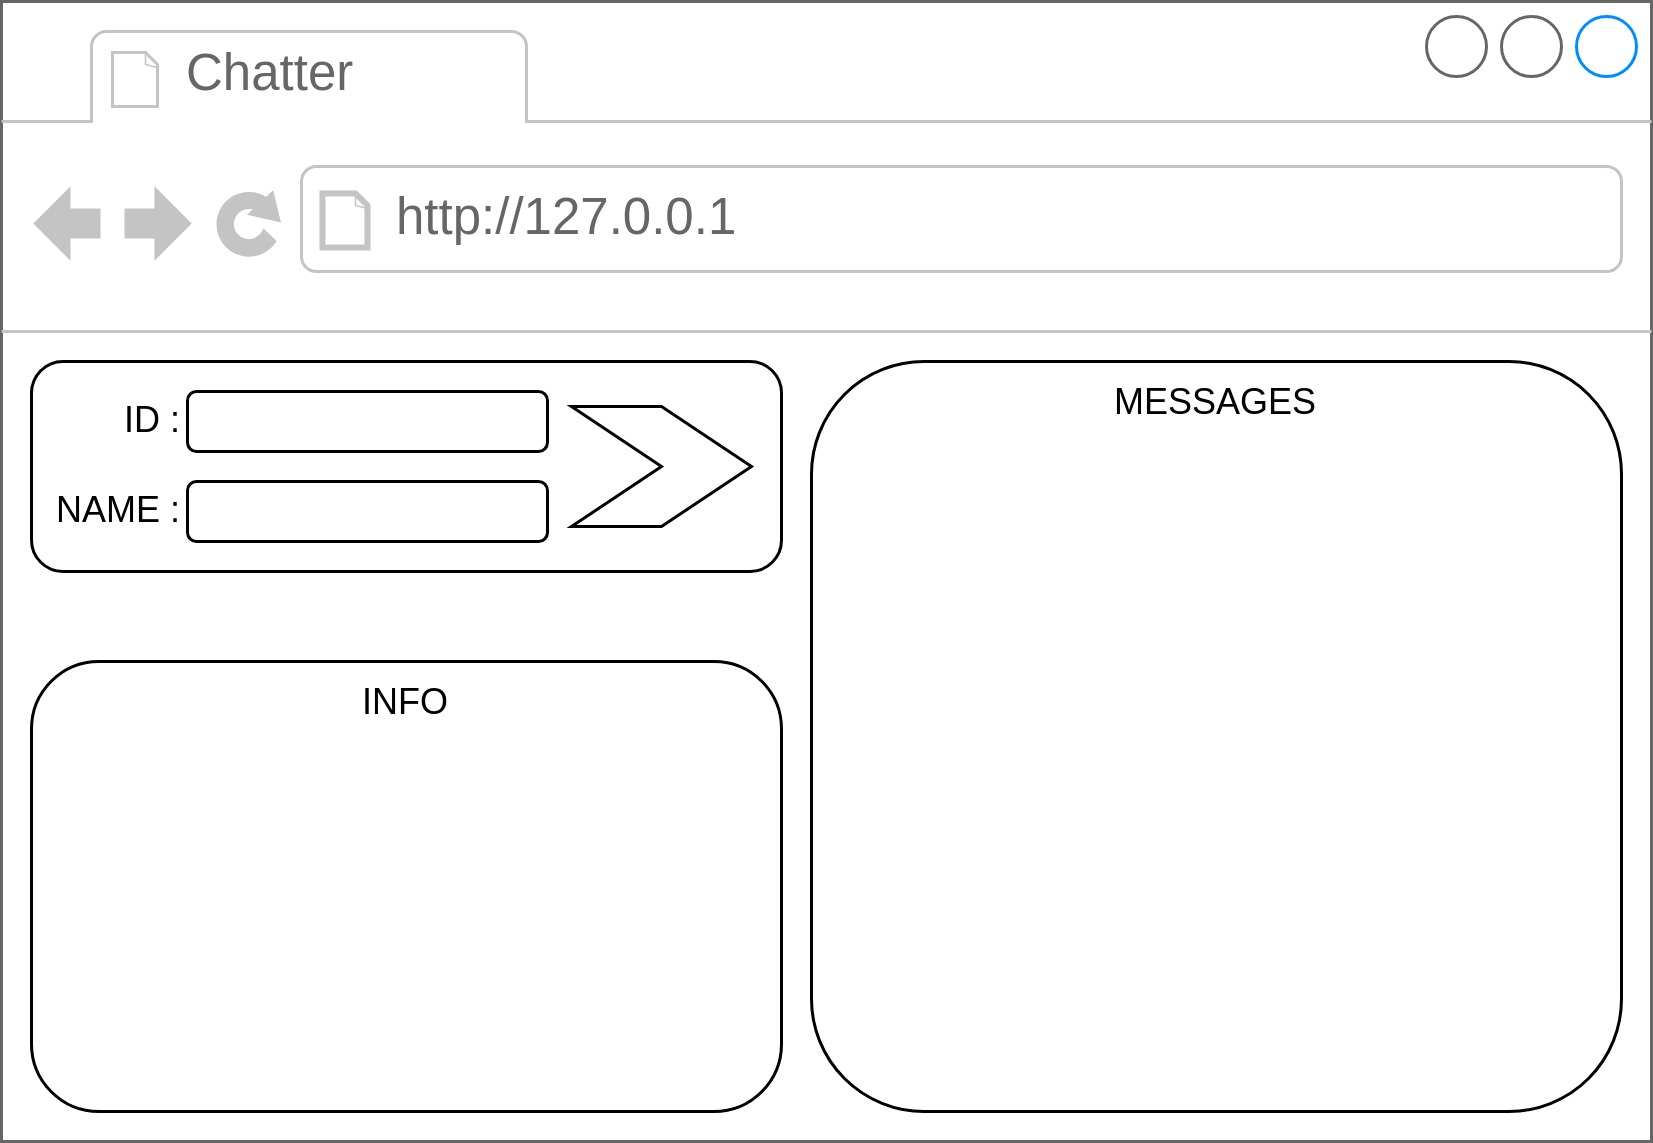
\includegraphics[width=5cm]{image/chatter-maquette}
    \end{frame}

    \begin{frame}{La DOM API}{Exercice \execcounterdispinc{}}
        \begin{itemize}
            \item Ajouter dans le script des messages à la classe \lstinline{Chatter}.
            \item À chaque message ajouté, mettre à jour la zone de droite qui affiche les messages.
        \end{itemize}
        \begin{dangercolorbox}
            Toujours utiliser la librairie CSS, bootstrap ou autre pour les nouveaux éléments, L'usage de JS ne doit pas détériorer le design de l'UI~.
        \end{dangercolorbox}
        \bigbreak
        \center
        \includegraphics[width=5cm]{image/chatter-maquette}
    \end{frame}

    \begin{frame}{La DOM API}{Exercice \execcounterdispinc{}}
        Ajouter un formulaire pour ajouter un message à \lstinline{Chatter} en haut de la card message.
        \begin{itemize}
            \item Un input pour ajouter le texte d'un message.
            \item L'input est \lstinline{disabled} par, mais activé dès qu'un \lstinline{Chatter} est instancié.
            \item Un bouton de soumission du formulaire.
            \item Un event \lstinline{click} ajoute le message à la classe \lstinline{Chatter}.
            \item La liste des messages est mise à jour.
        \end{itemize}
        \bigbreak
        \center
        \includegraphics[width=5cm]{image/chatter-maquette-2}
    \end{frame}


    \section{Communication}\label{sec:communication}

    \subsection{Généralités}\label{subsec:communication-basics}
    \begin{frame}{Les protocoles}{Généralités\footnote{\label{sendbird-protocole}Protocoles de communication WebSocket vs. HTTP, \url{https://sendbird.com/fr/developer/tutorials/websocket-vs-http-communication-protocols}}}
        HTTP est un protocole de communication semi-duplex, qui existe depuis un certain temps et constitue la base du Web depuis ses débuts.

        HTTP date de 1989, inventé au CERN par Tim Berners-Lee\footnote{The birth of the Web, \url{https://home.cern/science/computing/birth-web}}.
        \bigbreak
        WebSocket, un protocole de communication full-duplex, est relativement plus récent et convient mieux aux applications en temps réel (ou presque\ldots) comme le live chat dans les applications mobiles, les notifications et ou les appels audio ou vidéo.

        Websocket a été standardisé en 2011\footnote{The WebSocket Protocol, \url{https://datatracker.ietf.org/doc/html/rfc6455}}.
        Il est géré par le JavaScript du navigateur.
    \end{frame}

    \subsection{WebSocket}\label{subsec:websocket}

    \begin{frame}{Les protocoles}{Websocket, exercice \execcounterdispinc{}}
        \begin{itemize}
            \item Que veut dire full-duplex~?
            \item Y-a-t-il une contradiction avec une architecture client/serveur~?
            \item Citer un autre protocol full-duplex.
            \item Citer un protocol qui \textbf{n'est pas} full-duplex.
        \end{itemize}
        \bigbreak
        \centering
        \includegraphics[width=5cm]{image/homework}
    \end{frame}

    \begin{frame}{Les protocoles}{Websocket\cref{sendbird-protocole}}
        \centering
        \includegraphics[width=12cm]{image/tutorial-websocket-protocol-chart}
    \end{frame}

    \begin{frame}{Les protocoles}{Websocket côté client (Navigateur)\footnote{\label{mozilla-websocket}WebSockets, \url{https://developer.mozilla.org/fr/docs/Web/API/WebSockets_API}}}
        \begin{columns}
            \column{0.5\textwidth}
            \centering
            \includegraphics[width=3.3cm]{image/client-support} \\ Client \\
            \column{0.5\textwidth}
            \centering
            \includegraphics[width=6.5cm]{image/kids-on-the-phone}
        \end{columns}
    \end{frame}

    \begin{frame}{Les protocoles}{Websocket côté serveur (liste non exhaustive !)\cref{mozilla-websocket}}
        \begin{scriptsize}
            \begin{itemize}

                \item \href{https://github.com/uWebSockets/uWebSockets}{µWebSockets}~: Déclinaison plus légère et plus performante de WebSocket et écrite en \href{https://isocpp.org/}{C++11} et en \href{https://nodejs.org/fr/}{Node.js}.

                \item \href{https://github.com/ClusterWS/ClusterWS}{ClusteWS~}: Framework léger, rapide et puissant qui permet de construire des applications en \href{https://nodejs.org/fr/}{Node.js}.

                \item \href{http://socket.io}{Socket.IO}~: API WebSocket puissante et multiplateforme en \href{https://nodejs.org}{Node.js}.

                \item \href{https://socketcluster.io/\#!/}{SocketCluster}~: Framework open source en temps réel en \href{https://nodejs.org}{Node.js}.

                \item \href{https://nodejs.org}{Node.js}.

                \item \href{https://www.totaljs.com/}{Total.js}~: FrameWork pour web application en \href{https://nodejs.org}{Node.js}.

                \item \href{https://www.npmjs.com/package/faye-websocket}{Faye}~: Combine WebSocket(bidirectionnelle) et EventSource(unidirectionnelle), côté serveur et côté client en \href{https://nodejs.org}{Node.js}.

                \item \href{https://signalr.net/}{SignalR}~: SignalR est une nouvelle bibliothèque pour les développeurs \href{https://dotnet.microsoft.com/apps/aspnet}{ASP.NET}.

                \item \href{https://caddyserver.com/docs/websocket}{Caddy}~: Serveur web capable de créer des WebSockets serveur/proxy(stdin/stdout, echo, cat, \ldots).

                \item \href{https://github.com/websockets/ws}{ws}~: La plus populaire des WebSockets pour client \& serveur en \href{https://nodejs.org}{Node.js}.

                \item \href{https://github.com/bigstepinc/jsonrpc-bidirectional}{jsonrpc-bidirectional}~: Implémentation de JSON-RPC 2.0 sur WebSocket.

                \item \href{https://github.com/ninenines/cowboy}{cowboy}~: Cowboy est un petit serveur HTTP rapide et moderne pour Erlang/OTP basé sur WebSocket.

                \item \href{https://zeromq.org}{ZeroMQ}~: ZeroMQ est une bibliothèque de fonctions pour transporter des messages avec divers protocoles IPC, TCP, UDP, TIPC, diffusion de groupe et WebSocket.

            \end{itemize}
        \end{scriptsize}
    \end{frame}

    \begin{frame}{Websocket}{Exercice \execcounterdispinc{}}
        Tester et expliquer ce que font~:
        \begin{itemize}
            \item Le fichier \lstinline{server.js}.
            \item Le fichier \lstinline{ws.html}.
        \end{itemize}
        \bigbreak
        \centering
        \includegraphics[width=3cm]{image/intelligence}
    \end{frame}

    \subsection{HTTP}\label{subsec:http}

    \begin{frame}{Les protocoles}{HTTP\cref{sendbird-protocole}}
        \centering
        \includegraphics[width=12cm]{image/Tutorial-HTTP-connection-chart}
    \end{frame}

    \subsection{WebSocket VS HTTP}\label{subsec:ws-vs-http}

    \begin{frame}{Les protocoles}{HTTP\cref{sendbird-protocole}}
        \centering
        \includegraphics[width=12cm]{image/Tutorial-WebSocket-vs.-HTTP-communication-diagram}
    \end{frame}

    \begin{frame}{HTTP}{Introduction aux méthodes HTTP\footnote{\label{mozilla-http-methods}Méthodes de requête HTTP, \url{https://developer.mozilla.org/fr/docs/Web/HTTP/Methods}}}
        \begin{itemize}
            \item HTTP définit des méthodes de requête pour interagir avec les ressources.
            \item Ces méthodes sont souvent appelées \textit{verbes HTTP}.
            \item Les méthodes partagent parfois des fonctionnalités comme la \textit{sécurité}, l'\textit{idempotence}, ou la possibilité d'être \textit{mise en cache}.
        \end{itemize}
    \end{frame}

    \begin{frame}{HTTP}{Méthodes courantes\cref{mozilla-http-methods}}
        \begin{itemize}
            \item \lstinline{GET} : Récupère une ressource, sans modifier l'état du serveur (idempotence).
            Autorisée dans les \lstinline{<form>} HTML. Des données peuvent être envoyées dans l'URL~.
            \item \lstinline{HEAD} : Similaire à \lstinline{GET}~, sans le corps de la réponse.
            \item \lstinline{POST} : Envoie des données dans le corps de la requête, créant ou modifiant une ressource.
            Autorisée dans les \lstinline{<form>} HTML~.
            \item \lstinline{PUT} : Remplace la ressource avec les données envoyées.
            \item \lstinline{DELETE} : Supprime une ressource.
        \end{itemize}
        \begin{dangercolorbox}
            \lstinline{POST} et \lstinline{GET} sont compatibles avec les formulaires, mais à quoi donc servent alors les autres~?
        \end{dangercolorbox}
    \end{frame}

    \begin{frame}{HTTP}{Autres méthodes\cref{mozilla-http-methods}}
        \begin{itemize}
            \item \lstinline{CONNECT} : Établit un tunnel vers le serveur cible.
            \item \lstinline{OPTIONS} : Renvoie les options de communication avec la ressource.
            \item \lstinline{TRACE} : Effectue un test aller-retour sur le chemin suivi.
            \item \lstinline{PATCH} : Applique des modifications partielles à une ressource.
        \end{itemize}
    \end{frame}

    \begin{frame}{HTTP}{Introduction à Content-Type\footnote{\label{mozilla-content-type}Content-Type, \url{https://developer.mozilla.org/fr/docs/Web/HTTP/Headers/Content-Type}}}
        \begin{itemize}
            \item \textbf{Content-Type} : Indique le type MIME de la ressource.
            \item Utilisé dans les réponses pour informer le client du type de contenu renvoyé.
            \item Utilisé dans les requêtes POST/PUT pour indiquer au serveur le type de données envoyées.
        \end{itemize}
        \bigbreak
        Pourquoi pas dans les GET~?
        \pause
        La donnée est toujours dans l'URL et non dans le corps de la requête comme pour le POST~.
        C'est donc inutile.
    \end{frame}

    \begin{frame}{HTTP}{Directives de Content-Type\cref{mozilla-content-type}}
        \begin{itemize}
            \item \lstinline{media-type} : Type MIME des données.
            \item \lstinline{charset} : Encodage des caractères.
            \item \lstinline{boundary} : Limites pour les entités multipart.
        \end{itemize}
    \end{frame}

    \begin{frame}[fragile]{HTTP}{Exemple : Formulaires HTML\cref{mozilla-content-type}}
        \begin{lstlisting}[language=HTML]
<form action="/" method="post" enctype="multipart/form-data">
  <input type="text" name="description" value="du texte" />
  <input type="file" name="monFichier" />
  <button type="submit">Envoyer</button>
</form>
        \end{lstlisting}
        \begin{itemize}
            \item Requête POST envoyée avec Content-Type multipart/form-data.
        \end{itemize}
        \begin{lstlisting}[language=HTML]
<form action="/recherche" method="get">
    <input type="text" name="q" value="recherche" />
    <button type="submit">Rechercher</button>
</form>
        \end{lstlisting}
        \begin{itemize}
            \item Requête GET envoyée avec Content-Type application/x-www-form-urlencoded.
        \end{itemize}

    \end{frame}


    \begin{frame}{Tableau des codes de statut HTTP\footnote{Codes de réponse HTTP, \url{https://developer.mozilla.org/fr/docs/Web/HTTP/Status}}}
        \begin{tabular}{|p{1.5cm}|p{9.5cm}|}
            \hline
            \textbf{Code} & \textbf{Description}                                                         \\
            \hline
            100-199       & Réponses informatives (e.g. 100 Continue, 101 Switching Protocols)           \\
            \hline
            200-299       & Succès (e.g. 200 OK, 201 Created)                                            \\
            \hline
            300-399       & Redirections (e.g. 301 Moved Permanently, 302 Found)                         \\
            \hline
            400-499       & Erreurs client (e.g. 400 Bad Request, 404 Not Found, 405 Method Not Allowed) \\
            \hline
            500-599       & Erreurs serveur (e.g. 500 Internal Server Error, 503 Service Unavailable)    \\
            \hline
        \end{tabular}
    \end{frame}

    \subsection{L'API fetch}\label{subsec:fetch-api}

    \begin{frame}{Introduction à l'API \lstinline{fetch}\footnote{\label{mozilla-fetch}Fetch API, Mozilla, \url{https://developer.mozilla.org/fr/docs/Web/API/Fetch_API/Using_Fetch}}}
        \begin{itemize}
            \item L'API \lstinline{fetch} fournit une interface JavaScript pour accéder et manipuler des requêtes et réponses HTTP~.
            \item Elle utilise les promesses pour gérer les opérations asynchrones.
            \item L'API \lstinline{fetch} est une alternative moderne à XMLHttpRequest.
            \item Elle permet une gestion plus simple et plus puissante des requêtes HTTP~.
        \end{itemize}
        \bigbreak
        \centering
        \includegraphics[width=4cm]{image/http-tunnel}
    \end{frame}

    \begin{frame}{Qu'est-ce qu'une Promesse ?}
        \begin{itemize}
            \item Une Promesse est un objet représentant l'achèvement ou l'échec éventuel d'une opération asynchrone.
            \item Trois états possibles :
            \begin{itemize}
                \item \textbf{Pending} (en attente) : initial, ni résolu ni rejeté.
                \item \textbf{Fulfilled} (résolu) : l'opération a réussi.
                \item \textbf{Rejected} (rejeté) : l'opération a échoué.
            \end{itemize}
        \end{itemize}
        \bigbreak
        \centering
        \includegraphics[width=5cm]{image/promise}
    \end{frame}

    \begin{frame}[fragile]{Syntaxe : async, await, then, catch}
        \begin{itemize}
            \item \lstinline{async} : permet de définir une fonction asynchrone.
            \item \lstinline{await} : pause l'exécution de la fonction asynchrone jusqu'à ce que la Promesse soit résolue.
            \item \lstinline{then} : méthode pour gérer la résolution de la Promesse.
            \item \lstinline{catch} : méthode pour gérer le rejet de la Promesse.
        \end{itemize}
        \begin{lstlisting}[language=JavaScript,title={\tiny{Script JavaScript}}]
async function fetchData() {
    try {
        const response = await fetch("https://api.coinbase.com/v2/exchange-rates?currency=BTC");
        const data = await response.json();
        console.log(data);
    } catch (error) {
        console.error('Erreur:', error);
    }
}
fetchData().then(
    () => console.log('Données récupérées')
); // Pas de catch, car les erreurs sont esceptées, ça fonctionne toujours
        \end{lstlisting}
    \end{frame}

    \begin{frame}[fragile]{Syntaxe : async, await, then, catch\cref{mozilla-fetch}}
        Une promise qui ne fonctionne pas, on passe dans catch.
        \begin{lstlisting}[language=JavaScript,title={\tiny{Script JavaScript}}]
async function fetchData() {
    // NOTEZ QUE L'ADRESSE EST FAUT C'EST COIASE AU LIEU DE COINBASE
    const response = await fetch("https://api.coiase.com/v2/exchange-rates?currency=BTC");
    const data = await response.json();
    console.log(data);
}
fetchData().then(
    () => console.log('Données récupérées')
).catch(
    () => console.log('Erreur de fetch')
);
console.log("Juste après l'appel à fetchData")
        \end{lstlisting}
    \end{frame}

    \begin{frame}[fragile]{Faire une requête\cref{mozilla-fetch}}
        \begin{itemize}
            \item Utilisation de la méthode \lstinline{fetch()}.
            \item Exemple de requête GET, la requête par défaut :
        \end{itemize}
        \begin{lstlisting}[language=JavaScript,title={\tiny{Script JavaScript}}]
async function btcData() {
    const reponse = await fetch("https://api.coinbase.com/v2/exchange-rates?currency=BTC");
    const btc = await reponse.json();
    console.log(btc);
    return btc
}
btc = await btcData();
        \end{lstlisting}
    \end{frame}

    \begin{frame}[fragile]{Options de la requête\cref{mozilla-fetch}}
        \begin{itemize}
            \item La méthode \lstinline{fetch()} accepte un deuxième paramètre optionnel pour configurer la requête.
            \item Exemple de requête POST :
        \end{itemize}
        \begin{lstlisting}[language=JavaScript,title={\tiny{Script JavaScript}}]
async function postData(url = "", donnees = {}) {
    const response = await fetch(url, {
        method: "POST",
        mode: "cors",
        cache: "no-cache",
        credentials: "same-origin",
        headers: {
            "Content-Type": "application/json",
        },
        redirect: "follow",
        referrerPolicy: "no-referrer",
        body: JSON.stringify(donnees),
    });
    return response.json();
}
        \end{lstlisting}
    \end{frame}

    \begin{frame}{Le serveur \lstinline{ChatServer.js}}
        Permet de stocker les informations relatives aux Chatters et à leurs messages.
        \bigbreak
        C'est une API JSON couplée à une base de données.
        \bigbreak
        \centering
        \includegraphics[width=6cm]{image/api-server}
    \end{frame}

    \begin{frame}{Routes \lstinline{GET} du serveur \lstinline{ChatServer.js}}
        \begin{small}
            \begin{itemize}
                \item \textbf{GET /}
                \begin{itemize}
                    \begin{tiny}
                        \item Description: Retourne un message de bienvenue.
                        \item Méthode: \lstinline{app.get('/')}
                    \end{tiny}
                \end{itemize}
                \item \textbf{GET /v1/:userId/messages}
                \begin{itemize}
                    \begin{tiny}
                        \item Description: Récupère tous les messages d'un utilisateur.
                        \item Méthode: \lstinline{app.get('/v1/:userId/messages')}
                    \end{tiny}
                \end{itemize}
                \item \textbf{GET /v1/messages/last-hundred}
                \begin{itemize}
                    \begin{tiny}
                        \item Description: Récupère les 100 derniers messages de tous les utilisateurs.
                        \item Méthode: \lstinline{app.get('/v1/messages/last-hundred')}
                    \end{tiny}
                \end{itemize}
                \item \textbf{GET /v1/:userId/messages/last-five}
                \begin{itemize}
                    \begin{tiny}
                        \item Description: Récupère les cinq derniers messages d'un utilisateur.
                        \item Méthode: \lstinline{app.get('/v1/:userId/messages/last-five')}
                    \end{tiny}
                \end{itemize}
                \item \textbf{GET /v1/message/:messageId}
                \begin{itemize}
                    \begin{tiny}
                        \item Description: Récupère un message par son ID.
                        \item Méthode: \lstinline{app.get('/v1/message/:messageId')}
                    \end{tiny}
                \end{itemize}
                \item \textbf{GET /v1/chatter/:id}
                \begin{itemize}
                    \begin{tiny}
                        \item Description: Récupère un utilisateur par son ID.
                        \item Méthode: \lstinline{app.get('/v1/chatter/:id')}
                    \end{tiny}
                \end{itemize}
            \end{itemize}
        \end{small}
    \end{frame}

    \begin{frame}{Routes \lstinline{POST} du serveur \lstinline{ChatServer.js}}
        \begin{small}
            \begin{itemize}
                \item \textbf{POST /v1/message}
                \begin{itemize}
                    \begin{tiny}
                        \item Description: Ajoute un nouveau message.
                        \item Méthode: \lstinline{app.post('/v1/message')}
                        \item Paramètres:
                        \begin{itemize}
                            \begin{tiny}
                                \item \lstinline{content} (string) - Le contenu du message.
                                \item \lstinline{id} (integer) - L'ID unique du message.
                                \item \lstinline{userId} (integer) - L'ID de l'utilisateur qui envoie le message.
                                \item \lstinline{userName} (string) - Nom de l'utilisateur qui envoie le message.
                                \item \lstinline{date} (date) - La date et l'heure d'envoi du message.
                            \end{tiny}
                        \end{itemize}
                    \end{tiny}
                \end{itemize}
                \item \textbf{POST /v1/chatter}
                \begin{itemize}
                    \begin{tiny}
                        \item Description: Ajoute un nouvel utilisateur.
                        \item Méthode: \lstinline{app.post('/v1/chatter')}
                        \item Paramètres:
                        \begin{itemize}
                            \begin{tiny}
                                \item \lstinline{name} (string) - Le nom de l'utilisateur.
                                \item \lstinline{id} (integer) - L'ID unique de l'utilisateur.
                                \item \lstinline{latitude} (float) - La latitude de la position de l'utilisateur.
                                \item \lstinline{longitude} (float) - La longitude de la position de l'utilisateur.
                                \item \lstinline{hostname} (string) - Le nom d'hôte de l'utilisateur.
                                \item \lstinline{isMobile} (boolean) - Indique si l'utilisateur utilise un appareil mobile.
                                \item \lstinline{messageNumber} (integer) - Le nombre de messages envoyés par l'utilisateur.
                            \end{tiny}
                        \end{itemize}
                    \end{tiny}
                \end{itemize}
            \end{itemize}
        \end{small}
    \end{frame}

    \begin{frame}{Communication client/serveur}{Exercice \execcounterdispinc{}}
        \begin{itemize}
            \item Lister les actions dans le script de \lstinline{Chatter} qui devraient faire des appels au serveur.
            \item Associer ces actions aux routes du serveur \lstinline{chatServer.js}.
            \item Résumer ces communications dans un schéma.
        \end{itemize}
        \bigbreak
        \centering
        \includegraphics[width=3cm]{image/question-mark}
    \end{frame}


    \begin{frame}{Développement de la communication}{Exercice \execcounterdispinc{}}
        \begin{itemize}
            \item Dans le script précédemment développé, en utilisant l'API \lstinline{fetch}, connecter \lstinline{Chatter} à l'API, donc à la base de données.
            Les données seront donc persistantes.
            \item Faire des tests et une démonstration.
        \end{itemize}
        \bigbreak
        \centering
        \includegraphics[width=6cm]{image/fireworks}
    \end{frame}


    \section{Licence CC}\label{sec:licence}

    \begin
    {frame}{Licence}{Licence Creative Commons}
        Support de cours sous licence Creative Commons BY-NC-ND~.
        \bigbreak
        Vous pouvez donc, partager, copier, distribuer le document.
        \bigbreak
        Attribution requise à PapIT SASU - Pas d’utilisation commerciale - Pas de modification
        \bigbreak
        \centering
        \includegraphics[width=5cm]{image/by-nc-nd-logo}
    \end{frame}

\end{document}
